\documentclass[sigplan,screen]{acmart}
%Marcelo: Removed this line as part of author instructions\documentclass[sigplan,10pt,review]{acmart}
\settopmatter{printfolios=true}

%% Conference information
%% Supplied to authors by publisher for camera-ready submission;
%% use defaults for review submission.

\setcopyright{acmcopyright}
\acmPrice{}
\acmDOI{10.1145/3192366.3192414}
\acmYear{2018}
\copyrightyear{2018}
\acmISBN{978-1-4503-5698-5/18/06}
\acmConference[PLDI'18]{39th ACM SIGPLAN Conference on Programming Language Design and Implementation}{June 18--22, 2018}{Philadelphia, PA, USA}

\startPage{1}
\pagenumbering{gobble}

%% Bibliography style
\bibliographystyle{ACM-Reference-Format}
%% Citation style
%\citestyle{acmauthoryear}  %% For author/year citations
%\citestyle{acmnumeric}     %% For numeric citations
%\setcitestyle{nosort}      %% With 'acmnumeric', to disable automatic
                            %% sorting of references within a single citation;
                            %% e.g., \cite{Smith99,Carpenter05,Baker12}
                            %% rendered as [14,5,2] rather than [2,5,14].
%\setcitesyle{nocompress}   %% With 'acmnumeric', to disable automatic
                            %% compression of sequential references within a
                            %% single citation;
                            %% e.g., \cite{Baker12,Baker14,Baker16}
                            %% rendered as [2,3,4] rather than [2-4].


%
\usepackage{amsthm}
\usepackage{amsmath}
%\usepackage{SIunits}            % typset units correctly
%\usepackage{courier}            % standard fixed width font
\usepackage[scaled]{helvet} % see www.ctan.org/get/macros/latex/required/psnfss/psnfss2e.pdf
\usepackage{url}                  % format URLs
\usepackage{listings}          % format code
\usepackage{xspace}
%\usepackage{nth}
%\usepackage{enumitem}      % adjust spacing in enums
%\usepackage[colorlinks=true,allcolors=blue,breaklinks,draft=false]{hyperref}   % hyperlinks, including DOIs and URLs in bibliography
% known bug: http://tex.stackexchange.com/questions/1522/pdfendlink-ended-up-in-different-nesting-level-than-pdfstartlink
%\newcommand{\doi}[1]{doi:~\href{http://dx.doi.org/#1}{\Hurl{#1}}}   % print a hyperlinked DOI

\usepackage{color}

\usepackage{paralist}

\usepackage{hhline}

\usepackage[ruled,noline,noend,linesnumbered]{algorithm2e}

\usepackage{hyperref}
\usepackage{cleveref}
\usepackage{graphicx}
\usepackage{alltt}

\usepackage{amssymb}
\usepackage{amsmath}
\usepackage{xcolor}
\usepackage{listings}
%\usepackage{syntax}
\usepackage{semantic}
\usepackage[rightcaption]{sidecap}
\sidecaptionvpos{figure}{c}

\usepackage{flushend}

%% \newtheorem{theorem}{Theorem}[section]
%% \newtheorem{fact}[theorem]{Fact}
%% \newtheorem{lemma}[theorem]{Lemma}
%% \newtheorem{corollary}[theorem]{Corollary}
%% \newtheorem{proposition}[theorem]{Proposition}
%% %\newtheorem{lemma}[theorem]{Lemma}
%% %\newtheorem{corollary}[theorem]{Corollary}
%% %\newtheorem{proposition}[theorem]{Proposition}

%% \theoremstyle{definition}
%% \newtheorem{definition}{Definition}
%% %\newtheorem{definition}[theorem]{Definition}

%% \theoremstyle{remark}
%% \newtheorem{remark}[theorem]{Remark}
%% \newtheorem{example}{Example}
%% %\newtheorem{remark}{Remark}
%% %\newtheorem{example}[theorem]{Example}
%% %\newtheorem{remark}[theorem]{Remark}
%% %\newtheorem{observation}{Observation}
%% %\newtheorem{notation}{Notation}

\newcommand{\hlight}[1]{\textcolor{red}{#1}}

\newcommand{\para}[1]{\vspace{0.2cm} {\em #1.}}

\newcommand{\til}{,\ldots,}
\newcommand{\etc}{,\ldots}
\newcommand{\Nat}{{\mathbb{N}}}

%\newcommand{\dom}[1]{dom({#1})}
\newcommand{\dom}{dom}
\newcommand{\ov}{\overline}
\renewcommand{\Box}{\fbox{\rule{0cm}{.04cm}\rule{.04cm}{0cm}}}
\renewcommand{\phi}{\varphi}
\newcommand{\suc}{\mbox{{\rm Suc}}}
\newcommand{\A}{{\cal A}}        % the first order structure A
\newcommand{\abs}[1]{ \vert #1 \vert }
\newcommand{\sland}{\;\land\;}
\newcommand{\sra}{\;\rightarrow\;}
\newcommand{\bigand}{\bigwedge}
\newcommand{\maxp}{{\max}'}
\newcommand{\free}{\mbox{{\rm free}}}
\newcommand{\qsep}{{\;\;}}  % the separator in a quantified formula
\newcommand{\from}{{\colon}}
\newcommand{\card}[1]{{\left\vert{#1}\right\vert}} % set cardinality
%\newcommand{\cone}{\!\uparrow}
\newcommand{\cone}[1]{{#1}^\uparrow}
%\newcommand{\compl}[1]{\overline{#1}}
\newcommand{\compl}[1]{\States\setminus {#1}}
\newcommand{\Pfin}[1]{\mathcal{P}_{\textit{fin}}(#1)}

\renewcommand{\implies}{{\Rightarrow}}
\newcommand{\liff}{{\;\leftrightarrow\;}}


%%%%% Programs

\renewcommand{\program}{\mathit{Prog}}
\newcommand{\Cmd}{\mathit{C}}
\newcommand{\Decls}{\mathit{decls}}
\newcommand{\vars}{{\ensuremath{\mathcal{V}}}}
\newcommand{\relations}{{\ensuremath{\mathcal{R}}}}
\newcommand{\functions}{{\ensuremath{\mathcal{F}}}}
\newcommand{\sorts}{{\ensuremath{\mathcal{S}}}}
\newcommand{\axioms}{{\ensuremath{\mathcal{A}}}}
\newcommand{\Identity}{id}
\newcommand{\eqdef}{\buildrel \mbox{\tiny\rm def} \over =}

\renewcommand{\wp}{\mathit{wp}}
%\newcommand{\sp}{\mathit{sp}}
\newcommand\substitute[3]{{{#1} \left[ #3 ~/~ #2 \right]}}
\newcommand{\unroll}[2]{{{#1^{\leq {#2}}}}}

\newcommand{\type}{\tau}

%%%%% First order

\newcommand{\true}{{\textit{true}}}
\newcommand{\false}{{\textit{false}}}
\newcommand{\vocabulary}{{\ensuremath{\Sigma}}}
\newcommand{\letter}{{a}}
\newcommand{\dvoc}[1]{{(#1,#1')}}
%\newcommand{\theory}{{\Gamma}}
\newcommand{\structures}{{\mbox{STRUCT}}}
\newcommand{\structOfVoc}[1]{{\structures[#1]}}
\newcommand{\structOfTheory}[2]{{\structures[#1,#2]}}
\newcommand{\struct}{{s}}
\newcommand{\Dom}{{D}}
\newcommand{\Int}{{\mathcal{I}}}
\newcommand{\diag}[1]{{\textit{Diag}(#1)}}
\newcommand{\subst}[2]{{\left\{#1 / #2\right\}}}

\newcommand{\conjecture}{\varphi}

%%%% transition system

\newcommand{\Class}{{\mathcal{C}}}
\newcommand{\Lclass}{{\mathcal{L}}}

\newcommand{\Init}{\phi_{0}}
%\newcommand{\PhiProp}{\phi_{\Property}}
\newcommand{\Bad}{Bad}
\newcommand{\Trans}{\tau}
\newcommand{\IndInv}{\varphi}
\newcommand{\Lset}{L}
\newcommand{\ToLset}[1]{{L({#1})}}
\newcommand{\INV}{\mathcal{I}}
%\newcommand{\Inv}[2]{{\INV[{#1},{#2}]}}
\newcommand{\Inv}{{\mathit{Inv}}}
\newcommand{\InvSet}[2]{{\INV[{#1},{#2}]}}
\newcommand{\SafeSet}[1]{{\texttt{SAFE}[{#1}]}}
\newcommand{\image}[1]{{\TR({#1})}}
\newcommand{\preimage}[1]{{\TR^{-1}({#1})}}
\newcommand{\TS}{{\textit{TS}}}
\newcommand{\TSr}[1]{\TS^{#1}}
\newcommand{\States}{S}
\newcommand{\InitStates}{{S_0}}
\newcommand{\TR}{{\tau}}
\newcommand{\TRr}[1]{\TR^{#1}}
\newcommand{\Property}{{\varphi_P}}
%\newcommand{\state}{s}
\newcommand{\reachStates}{{\textit{Reach}}}
\newcommand{\Istar}{{I^{*}}}
\newcommand{\TSlogic}{\TS}
\newcommand{\Invar}{I}

\newcommand{\BMC}{\text{BMC}}

%%%% L

\newcommand{\Univ}{{\forall^*}}
%\newcommand{\leqLof}[1]{{\leq_{#1}}}
\newcommand{\leqLof}[1]{\sqsubseteq_{#1}}
\newcommand{\leqL}{\leqLof{\Lset}}
\newcommand{\leqU}{\leqLof{\Univ}}
\newcommand{\leqTree}{\preceq}
%\newcommand{\leqTree}{\preccurlyeq}
\newcommand{\Avoid}{{\text{Avoid}}}
\newcommand{\AvoidOfL}[1]{{\text{Avoid}_{#1}}}
\newcommand{\AvoidL}{{\AvoidOfL{\Lset}}}
\newcommand{\AvoidLstate}[1]{{\AvoidL({#1})}}

%%%% Modeling language

\newcommand{\gV}[1]{\langle \textit{#1}\rangle}
\newcommand{\btuple}[1]{\overline{#1}}
\newcommand{\bvar}{\textbf{v}}
\newcommand{\brel}{\textbf{r}}
\newcommand{\bfun}{\textbf{f}}
\newcommand{\bsort}{\textbf{s}}
\newcommand{\binsert}{\texttt{insert}}
\newcommand{\bremove}{\texttt{remove}}
\newcommand{\babort}{\texttt{abort}}
\newcommand{\bskip}{\texttt{skip}}
\newcommand{\bdo}{\texttt{do}}
\newcommand{\bwhile}{\texttt{while}}
\newcommand{\bassume}{\texttt{assume}}
\newcommand{\bassert}{\texttt{assert}}
\newcommand{\bif}{\texttt{if}}
\newcommand{\bthen}{\texttt{then}}
\newcommand{\belse}{\texttt{else}}
\newcommand{\bite}{\texttt{ite}}

\newcommand{\cinit}{\Cmd_{\texttt{init}}}
\newcommand{\cbody}{\Cmd_{\texttt{body}}}
\newcommand{\cfinal}{\Cmd_{\texttt{final}}}
\newcommand{\phiinit}{\varphi_{\texttt{init}}}
\newcommand{\phiqf}{\varphi_{\texttt{QF}}}
\newcommand{\phiea}{\varphi_{\texttt{EA}}}
\newcommand{\phiae}{\varphi_{\texttt{AE}}}
\newcommand{\phiaf}{\varphi_{\texttt{AF}}}
\newcommand{\gVphiqf}{{\langle \phiqf \rangle}}
\newcommand{\gVphiea}{{\langle \phiea \rangle}}
\newcommand{\gVphiae}{{\langle \phiae \rangle}}
\newcommand{\gVphiaf}{{\langle \phiaf \rangle}}

\newcommand{\Nodes}{\text{Nodes}}

\newcommand{\IF}{\texttt{if}}
\newcommand{\THEN}{\texttt{then}}
\newcommand{\ELSE}{\texttt{else}}
\newcommand{\WHILE}{\texttt{while}}
%\newcommand{\LOOP}{\texttt{loop}}
%\newcommand{\INSERT}{\texttt{insert}}
%\newcommand{\INSERTM}[3]{\INSERT\,(#1.\texttt{insert}(#2, #3))}
%\newcommand{\INSERTM}[3]{#1.\texttt{insert}(#2 \mid #3))}
\newcommand{\INSERTM}[2]{#1 := #1 \cup \{ #2\}}
\newcommand{\INSERTMU}[3]{#1 := #1 \cup \{ #2 \mid #3 \}}
%\newcommand{\REMOVE}{\texttt{remove}}
%\newcommand{\REMOVEM}[3]{#1.\texttt{remove}(#2 \mid #3))}
\newcommand{\REMOVEM}[2]{#1 := #1 \setminus \{ #2 \}}
\newcommand{\REMOVEMU}[3]{#1 := #1 \setminus \{ #2 \mid #3 \}}
\newcommand{\ASSUME}{\texttt{assume}}
\newcommand{\ASSUMEM}[1]{\ASSUME\,#1}
\newcommand{\ASSERT}{\texttt{assert}}
\newcommand{\ASSERTM}[1]{\ASSERT\,#1}
\newcommand{\COMMENT}[1]{\texttt{\# #1}}
\newcommand{\INDENT}{\quad}


\newcommand{\Plink}{\textit{link}}
\newcommand{\Ptree}{\textit{tree}}
\newcommand{\Ptreestar}{{\textit{tree}^*}}
\newcommand{\Ppending}{\textit{pending}}
%\newcommand{\Pmarked}{\textit{marked}}
\newcommand{\Plearned}{\textit{learned}}

\newcommand{\mLink}{{\textit{link}}}
\newcommand{\mRoute}{{\textit{route}}}
\newcommand{\mRoutestar}{{\mRoute^*}}
\newcommand{\mPending}{{\textit{pending}}}
\newcommand{\mLearned}{{\textit{learned}}}

\newcommand{\rroot}{\mathit{root}}
%\newcommand{\sw}{\textit{sw}}
\newcommand{\sw}{\mathit{sw}}
\newcommand{\src}{\mathit{src}}
\newcommand{\dst}{\mathit{dst}}

%%%%%% RML

\newcommand{\sort}[1]{{\text{#1}}}
\newcommand{\snode}{\sort{node}}
\newcommand{\squorum}{\sort{quorum}}
\newcommand{\sround}{\sort{round}}
\newcommand{\svalue}{\sort{value}}
\newcommand{\sinst}{\sort{instance}}
\newcommand{\svotemap}{\sort{votemap}}
\newcommand{\snodeset}{\sort{nset.t}}
\newcommand{\smap}{\sort{map}}
\newcommand{\sfquorum}{\sort{f\_quorum}}
\newcommand{\scquorum}{\sort{c\_quorum}}
\newcommand{\sconfig}{\sort{config}}
\newcommand{\sint}{\sort{int}}
\newcommand{\Integer}{\sint}
\newcommand{\sterm}{\sort{term}}

\newcommand{\relation}[1]{{\text{#1}}}
\newcommand{\rvoted}{\relation{voted}}
\newcommand{\risleader}{\relation{isleader}}
\newcommand{\rmember}{\relation{member}}
\newcommand{\rmajority}{\relation{majority}}
\newcommand{\rlen}{\relation{array.len}}
\newcommand{\rvalue}{\relation{array.value}}
\newcommand{\rreachedset}{\relation{r}_\relation{s}}
\newcommand{\rreachednode}{\relation{r}_\relation{n}}
\newcommand{\risize}{\relation{card}}
\newcommand{\ralreadyvoted}{\relation{alreadyvoted}}
\newcommand{\rvoters}{\relation{voters}}
\newcommand{\rempty}{\relation{empty}}
\newcommand{\rall}{\relation{all}}
\newcommand{\rallnodes}{\snode.\rall}
\newcommand{\rallnodeset}{\relation{allnodes}}
\newcommand{\rquorum}{\relation{quorum}}
\newcommand{\msgrequestvote}{\relation{request\_vote\_msg}}
\newcommand{\msgvote}{\relation{vote\_msg}}
\newcommand{\msgleader}{\relation{leader\_msg}}


\newcommand{\action}[1]{{\text{#1}}}
\newcommand{\pvote}{\action{vote}}
\newcommand{\pbecomeleader}{\action{become\_leader}}
\newcommand{\prequestvote}{\action{request\_vote}}
\newcommand{\padd}{\action{add}}
\newcommand{\pemptyset}{\action{emptyset}}
\newcommand{\pinit}{\action{init}}
\newcommand{\pcastvote}{\action{cast\_vote}}
\newcommand{\preceivevote}{\action{receive\_vote}}

\newcommand{\module}[1]{{\text{#1}}}
\newcommand{\mtoyprotocol}{\module{toy\_protocol}}
\newcommand{\mtoysystem}{\module{toy\_system}}
\newcommand{\mnodeset}{\module{nset}}
\newcommand{\tnodeset}{\module{nodeset.t}}
\newcommand{\keyword}[1]{{\bf{#1}}}
\newcommand{\irule}[1]{{\textup{\textsc{#1}}}}

\newcommand{\invariant}[1]{{\text{#1}}}
\newcommand{\ioneleader}{\invariant{one\_leader}}
\newcommand{\iintersect}{\invariant{majorities\_intersect}}
\newcommand{\isafe}{\invariant{safe}}
\newcommand{\modinvar}{Q}


\newcommand{\self}{\text{self}}

%%%%%% quasi

\newcommand{\QR}{QR}

%%%%% Singly linked lists

\newcommand{\nstar}{{n^*}}
\newcommand{\mstar}{{m^*}}
\newcommand{\LinOrd}{{\theory_{\nstar}}}
%\newcommand{\next}{{next}}
\newcommand{\phinext}{{\phi_\next}}
\newcommand{\Vnstar}{{\vocabulary_{\nstar}}}
\newcommand{\T}{{\cal T}}
\newcommand{\Trees}[1]{{\T({#1})}}
\newcommand{\Tnstar}{{\T_\nstar}}
\newcommand{\Snstar}{{\structOfTheory{\Vnstar}{\LinOrd}}}

\newcommand{\Forests}[1]{{{\cal F}({#1})}}
\newcommand{\tree}{{T}}
\newcommand{\forest}{{F}}
\newcommand{\Root}{{root}}
\newcommand{\lroot}{{l_\Root}}
\newcommand{\phiroot}{{\phi_\Root}}
\newcommand{\vroot}{{v_\Root}}

%%%%% Backward Reachability

\newcommand{\reduceKw}{\mathit{reduct}}
\newcommand{\reduce}[1]{\reduceKw(#1)}
\newcommand{\SATKw}{\mathit{SAT}}
\newcommand{\SAT}[1]{\SATKw(#1)}
\newcommand{\findMinModelKw}{\mathit{min\mbox{-}model}}
\newcommand{\findMinModel}[1]{\findMinModelKw(#1)}
\newcommand{\findModelKw}{\mathit{model}}
\newcommand{\findModel}[1]{\findModelKw(#1)}

%%%%% Undecidability

\newcommand{\enc}{{\mathcal{E}}}
\newcommand{\inc}{\texttt{INC}}
\newcommand{\dec}{\texttt{DEC}}
\newcommand{\testzero}{\texttt{TEST-ZERO}}
\newcommand{\head}{{h}}
\newcommand{\tail}{{t}}
\newcommand{\OP}{{OP}}
\newcommand{\phiconfig}{{\phi_{config}}}
\newcommand{\phienc}{{\phi_\enc}}
\newcommand{\distinct}[1]{{\texttt{distinct}({#1})}}
\newcommand{\len}{{\ell}}
\newcommand{\goal}{{\mbox{goal}}}

%%%%% Abbrevs

\newcommand{\EPR}{\textsc{EPR}\xspace}
\newcommand{\SDN}{\textsc{SDN}\xspace}
\newcommand{\RML}{\textsc{RML}\xspace}

%%%%% Misc

\newcommand{\sharon}[1]{{\textcolor{blue}{SS: {\em #1}}}}
\newcommand{\oded}[1]{{\textcolor{brown}{OP: {\em #1}}}}
\newcommand{\ken}[1]{{\textcolor{cyan}{KLM: {\em #1}}}}
\newcommand{\TODO}[1]{{\textcolor{red}{TODO: {\em #1}}}}
\newcommand{\jrw}[1]{{\textcolor{violet}{JRW: {\em #1}}}}
\newcommand{\dw}[1]{{\textcolor{blue}{DW: {\em #1}}}}
\newcommand{\gl}[1]{{\textcolor{green}{GL {\em #1}}}}
\newcommand{\mooly}[1]{{\textcolor{yellow}{MS {\em #1}}}}
\newcommand{\commentout}[1]{}
\newcommand{\adam}[1]{{\textcolor{red}{AD {\em #1}}}}
\newcommand{\OMIT}[1]{}

 \renewcommand{\sharon}[1]{}
 \renewcommand{\oded}[1]{}
 \renewcommand{\TODO}[1]{}
 \renewcommand{\ken}[1]{}
 \renewcommand{\jrw}[1]{}
 \renewcommand{\gl}[1]{}
 \renewcommand{\dw}[1]{}
 \renewcommand{\adam}[1]{}
 \renewcommand{\mooly}[1]{}

\newcommand{\remove}[1]{\xspace}

\newcommand{\allnotes}[1]{}
% To make the FIXMEs go away, comment out this line...
%% \renewcommand{\allnotes}[1]{\textit{#1}}
%% \newcommand{\fixme}[1]{{\allnotes{\bf\textcolor{red}{[#1]}}}}
%% \newcommand{\notepanda}[1]{\allnotes{\textcolor{cyan}{[Panda: #1]}}}
\newcommand{\ie}{{\it i.e.,}\xspace}

%\newcommand{\Vars}[1]{\mbox{\em Vars}(#1)}
\newcommand{\Sorts}{\mathcal{S}}
\newcommand{\Bool}{\mathbb{B}}
\newcommand{\Vars}[1]{\vocabulary(#1)}
\newcommand{\Before}[2]{(#2 \triangleright #1)}
\newcommand{\After}[2]{(#1 \triangleright #2)}
\newcommand{\Names}{\mathcal{N}}
\newcommand{\Stat}{\mathcal{S}}
\newcommand{\Prop}{\mathcal{P}}
\newcommand{\Logic}{\mathcal{L}}
\newcommand{\Hoare}{\mathcal{H}}
\newcommand{\Domain}{\mbox{\rm pre}}
\newcommand{\Codomain}{\mbox{\rm img}}
\newcommand{\Called}{\mbox{\rm called}}
\newcommand{\ModInvar}{\mathcal{I}}
\newcommand{\Asgn}{\mbox{:=}}
\newcommand{\Restr}{\downarrow}
\newcommand{\Ref}{\mbox{\rm ref}}
\newcommand{\Mod}{\mbox{\rm mod}}
\newcommand{\CallSet}{\mbox{\rm calls}}
\newcommand{\PreAssume}[2]{[#2]#1}
\newcommand{\PostAssume}[2]{#1[#2]}


\newcommand{\Interf}{\leadsto}
\newcommand{\Abs}[1]{{#1}\uparrow}
\newcommand{\Comp}{+}
\newcommand{\Compat}{\smile}
\newcommand{\Layer}{Layer}
\newcommand{\Slice}[1]{\mbox{\rm slice}(#1)}
\newcommand{\bra}[1]{\left\{#1\right\}\ }
\newcommand{\ket}[1]{\ \left\{#1\right\}}
\newcommand{\Vocab}{\mathcal{V}}
\newcommand{\Sig}{\Sigma}
\newcommand{\PVars}{\Vocab_{P}}
\newcommand{\Msg}{\mu}
\newcommand{\Msgs}{\mathcal{M}}
\newcommand{\Sent}{\mbox{sent}}
\newcommand{\Pid}{\mbox{pid}}
\newcommand{\Recv}[1]{\mbox{recv}_{#1}}
\newcommand{\Toy}{Toy Leader Election}
\newcommand{\Lang}{MDL}
\newcommand{\srt}{\textsf{srt}}
\newcommand{\theory}{T}

% setting for lstlisting
\lstset{ %
%  backgroundcolor=\color{white},   % choose the background color; you must add \usepackage{color} or \usepackage{xcolor}
%  basicstyle=\scriptsize,        % the size of the fonts that are used for the code
%  basicstyle=\normalsize,        % the size of the fonts that are used for the code
  breakatwhitespace=false,         % sets if automatic breaks should only happen at whitespace
%  breaklines=true,                 % sets automatic line breaking
%  captionpos=b,                    % sets the caption-position to bottom
%  commentstyle=\color{mygreen},    % comment style
%  deletekeywords={...},            % if you want to delete keywords from the given language
%  escapeinside={\%*}{*)},          % if you want to add LaTeX within your code
%  extendedchars=true,              % lets you use non-ASCII characters; for 8-bits encodings only, does not work with UTF-8
  frame=single,                    % adds a frame around the code
%  keepspaces=true,                 % keeps spaces in text, useful for keeping indentation of code (possibly needs columns=flexible)
  keywordstyle=\bf,       % keyword style
  language=C,                 % the language of the code
  otherkeywords={module,ghost,invariant,uses,procedure,requires,ensures,system,message,send,handles,type,interpret,as,individual,init,action,returns,assert,assume,instantiate,isolate,mixin,before,relation,function,sort,variable,axiom,then,constant,let,*,local,open},           % if you want to add more keywords to the set
  numbers=left,                    % where to put the line-numbers; possible values are (none, left, right)
  numbersep=5pt,                   % how far the line-numbers are from the code
  numberstyle=\tiny,               % the style that is used for the line-numbers
  rulecolor=\color{black},         % if not set, the frame-color may be changed on line-breaks within not-black text (e.g. comments (green here))
%  showspaces=false,                % show spaces everywhere adding particular underscores; it overrides 'showstringspaces'
%  showstringspaces=false,          % underline spaces within strings only
%  showtabs=false,                  % show tabs within strings adding particular underscores
%  stepnumber=2,                    % the step between two line-numbers. If it's 1, each line will be numbered
%  stringstyle=\color{mymauve},     % string literal style
  tabsize=8,                       % sets default tabsize to 2 spaces
%  title=\lstname                   % show the filename of files included with \lstinputlisting; also try caption instead of title
   columns=fullflexible,
}


\begin{document}

%\title{Decidable Reasoning about Distributed Systems Implementations}
%\title[Modularity for Decidability]{Modularity for Decidability: Verifying Distributed Systems Implementations}
%\title[Modularity for Decidability]{Modularity for Decidability: Implementing and Semi-Automatically Verifying Distributed Systems}
\title[Modularity for Decidability]{Modularity for Decidability of Deductive Verification with Applications to Distributed Systems}
\author{Marcelo Taube}
\affiliation[obeypunctuation]{
  \institution{Tel Aviv University},
  \country{Israel}
}
\email{mail.marcelo.taube@gmail.com}

\author{Giuliano Losa}
\affiliation[obeypunctuation]{
  \institution{UCLA},
  \country{USA}
  %
}
\email{giuliano@cs.ucla.edu}

\author{Kenneth L. McMillan}
\affiliation[obeypunctuation]{
  \institution{Microsoft Research},
  \country{USA}
  %
}
\email{kenmcmil@microsoft.com}

\author{Oded Padon}
\affiliation[obeypunctuation]{
    \institution{Tel Aviv University},
    \country{Israel}
    %
}
\email{odedp@mail.tau.ac.il}

\author{Mooly Sagiv}
\affiliation[obeypunctuation]{
  \institution{Tel Aviv University},
  \country{Israel}
%
}
\email{msagiv@post.tau.ac.il}

\author{Sharon Shoham}
\affiliation[obeypunctuation]{
  \institution{Tel Aviv University},
  \country{Israel}
  %\country{Israel}
}
\email{sharon.shoham@gmail.com}

\author{James R. Wilcox}
\affiliation[obeypunctuation]{
    \institution{University of Washington},
    \country{USA}
    %\country{USA}
}
\email{jrw12@cs.washington.edu}

\author{Doug Woos}
\affiliation[obeypunctuation]{
    \institution{University of Washington},
    \country{USA}
    %\country{USA}
}
\email{dwoos@cs.washington.edu}

\renewcommand{\shortauthors}{M. Taube et al.}

\begin{abstract}

\commentout{
This paper addresses the problem of verifying the correctness of realistic distributed systems, all the way from
protocol design to efficient system implementation.
\gl{implementations}\oded{is this better?}
It shows how to harness modularity for simplifying the verification of such systems.
Rather then directly reasoning about existing code,
we present a programming language which both permits effective
reasoning and generation of efficient executable code.

The simplification is achieved by the usage of decidable logic to automatically check the correctness of straightline programs.
Unlike existing approaches, the usage of decidable logic guarantees that the solver always terminates with a proof or a concrete counterexample.
However, decidable logics are not a panacea. They are rather limited and common wisdom suggests that it is very hard to employ decidable reasoning to reason
about real systems.

This paper shows that existing modularity principles can be used to break the verification task into several subtasks that can be solved
via different decidable logics.
We embed this modularity in a real verification system and demonstrate the usefulness of the methodology
to verify realistic protocols, such as Raft, all the way from the design to an efficient implementation.
We also show that the verification effort is drastically smaller than existing approaches.

There are several reasons why this can be done for distributed systems:
(i)~The existence of a rather simple design of the protocol expressible in a rather limited language,
(ii)~The separation between abstract and concrete data structures, and
(iii)~The message passing communication model which makes it possible to treat each message handler as executing atomically.
}

Proof automation can substantially increase productivity in formal
verification of complex systems.  However, unpredictablility of automated provers in handling quantified formulas presents a major
hurdle to usability of these tools. We propose to solve this
problem not by improving the provers, but by using a modular proof
methodology that allows us to produce \emph{decidable} verification
conditions.  Decidability greatly improves predictability of proof
automation, resulting in a more practical verification approach. 
We apply this methodology to develop verified
implementations of distributed protocols, demonstrating its effectiveness.

%We
%demonstrate this by using the methodology to develop verified
%implementations of distributed protocols with competitive performance.


%\item The isolation between the local states at every node.

%\begin{inparaenum}[(i)]
%\item The existence of a rather simple design of the protocol expressible in a rather limited language,
%\item The separation between abstract and concrete data structures, and
%\item The message passing communication model which makes it possible to treat each message handler as executing atomically.
%%\item The isolation between the local states at every node.
%\end{inapraenum}


%
%
%
% \oded{I just put this here for us, we should write a real
%abstract} We consider challenging distributed systems, e.g., Raft,
%Muti-Paxos, Sharded Hash Table. We develop a methodology to
%strucutre both the systems implementation and its proof such that
%verification conditions are in decidable logics. We show that this
%resutls in shorted and more intuitive proofs, as well as predictable
%automation of VC checks.
\end{abstract}


\begin{CCSXML}
<ccs2012>
<concept>
<concept_id>10011007.10011074.10011099.10011692</concept_id>
<concept_desc>Software and its engineering~Formal software verification</concept_desc>
<concept_significance>500</concept_significance>
</concept>
</ccs2012>
\end{CCSXML}

\ccsdesc[500]{Software and its engineering~Formal software verification}
%\ccsdesc[300]{Computer systems organization~Dependable and fault-tolerant systems and networks}

\keywords{Formal verification, Modularity, Decidable logic, Ivy, Distributed systems, Paxos, Raft}

\maketitle

%\oded{for the final version: use ``decidable decomposition'' more often, maybe instead of theory segregation}
\section{Introduction}

\begin{sloppypar}
Verifying complex software systems is a longstanding research goal.
Recently there have been some success stories in verifying
compilers~\cite{Compcert}, operating systems~\cite{sel4}, and
distributed systems~\cite{IronFleet,Verdi}.  These broadly use two
techniques: interactive theorem proving (e.g., Coq~\cite{coq},
Isabelle/HOL~\cite{nipkow_isabelle/hol:_2002}) and deductive
verification based on automated theorem provers (e.g.,
Dafny~\cite{Dafny} which uses Z3~\cite{Z3}). However, both techniques
are difficult to apply and require a large proof engineering effort.
On the one hand, interactive theorem provers allow a user to write
proofs in highly expressive formalisms (e.g., higher-order logic or
dependent type theory).  While this allows great flexibility, it
generally requires the user to manually write long and detailed
proofs.
\end{sloppypar}

On the other hand, deductive verification techniques use automated theorem provers
%,e.g. the Z3 SMT solver~\cite{Z3}\mooly{why do we refer to Z3 and not to other SMTs},
to reduce the size of the manually written proofs. In this approach,
user-provided annotations (e.g., invariants, pre- and post-conditions)
are used to reduce the proof to
lemmas called \emph{verification conditions} that can be discharged by
the automated prover.  In case these lemmas fail, the prover can
sometimes produce counterexamples that explain the failure and allow
the programmer to correct the annotations.

Unfortunately, the behavior of provers can be quite unpredictable,
especially when applied to formulas with quantifiers, which are common
in practice, e.g., in distributed systems. Since the problem presented to
the prover is in general undecidable, it is no surprise that the
prover sometimes diverges or produces inconclusive results on small
instances, or suffers from the ``butterfly effect'', when a seemingly
irrelevant change in the input causes the prover to fail. As observed
in the IronFleet project, SMT solvers can diverge even on tiny
examples~\cite{IronFleet}. When this happens, the user has little information with
which to decide how to proceed.  This was identified in IronFleet as
the main hurdle in the verification task.

One approach to address the unpredictability of automated solvers is
to restrict verification conditions to a decidable fragment of
logic~\cite{dragoi_psync:_2016,DBLP:conf/tacas/HenriksenJJKPRS95,SmallFootDecidable,MadhusudanPQ11}.
%\TODO{Mooly, can you check the references? what else should we cite here? I couldn't figure out citations to: nyad, everything-else}
Our previous work on the Ivy verification system~\cite{Ivy,
  ken_fmcad16, oopsla17-epr} has used the effectively propositional
(EPR) fragment of first-order logic to verify distributed protocols
designs (e.g. cache coherence and consensus). However, the
restrictions imposed for decidability are a major limitation. In
particular, these restrictions are the reason our previous works only
verified protocol designs rather than their executable
implementations.
%\oded{Can you check the last few sentences? Marcelo and I rewrote them following Adam's comment}

\paragraph{Decidable Decomposition}

In this paper, we show how to use well-understood modular reasoning
techniques to increase the applicability of decidable reasoning
and support verifying implementations as well as designs.
The key idea is to structure the correctness proof in a modular way,
such that each component can be proved using a decidable fragment of first-order logic,
possibly with a background theory. Importantly, each component's
verification condition can use a \emph{different} decidable fragment.
This allows, for example, one component to use arithmetic, while another uses
stratified quantifiers and uninterpreted relations. It also allows
each component to use its own quantifier stratification, even when
the combination would not be stratified. We will refer to
this approach as \emph{decidable decomposition}.  Crucially, decidable
decomposition can be applied even when the global verification
condition does not lie in any single decidable fragment (for example,
the combination of arithmetic, uninterpreted relations, and
quantifiers is undecidable).

% A key aspect of our methodology is the separation between the abstract
% model and its implementation using concrete data
% structures. We prove system-level properties of the protocol using the
% abstract model and use these properties as a lemma in proving the
% implementation. This is important for obtaining stratification in the use of quantifiers.
% In addition, we use abstract datatypes to hide the
% theory needed to implement a data structure behind a set of abstract
% properties. The resulting
% decidable decomposition allows us to prove each
% module locally with decidable logics, even though a global proof would take us
% outside the decidable range.

Because our prover is a decision procedure for the logical fragments
we use, we can guarantee that in principle it will always terminate
with a proof or a counter-model. In practice, decidability means that
the behavior of the prover is much more predictable.



\paragraph{Verifying Distributed Systems}

As a demonstration of decidable decomposition, we verify distributed protocols and
their implementations. %\oded{I rephrased the following}
Distributed protocols play an essential role in today's computing landscape.
Reasoning about distributed protocols naturally leads to quantifiers and uninterpreted relations,
while their implementations use both arithmetic and concrete
representations (e.g., arrays). This combination escapes known decidable fragments. In particular, it prevented our previous work on the Ivy verification system from verifying
the implementations of distributed protocols.
%To overcome this, we use decidable decomposition in this work.
Here, we overcome this by applying decidable decomposition.

%but our previous work on the Ivy verification system could not verify
%their implementations. \sharon{remove "but our previous work on the Ivy verification system could not verify
%their implementations" (it's repetitive. but if we do want to repeat, it makes sense to repeat towards the end of the paragraph when saying "escapes...").  Also remove the words "In particular" but keep the rest of the sentence }In particular, reasoning about distributed
%protocols naturally leads to quantifiers and uninterpreted relations,
%while their implementations use both arithmetic and concrete
%representations (e.g., arrays). This combination escapes the decidable
%fragments used in previous work. \sharon{replace "the decidable
%fragments used in previous work" by "known decidable
%fragments". Possibly add "preventing our previous work on the Ivy verification system from verifying
%the implementations of distributed protocols."}
%\sharon{append "To overcome this, we use decidable decomposition" (otherwise the connection with next paragraph is too loose)}

We observe in our evaluation that the human effort needed to achieve
decidable decomposition is modest, and follows well known modular design principles.
%We identify a few patterns \sharon{do we ever go back to the patterns? }that
%suffice to decompose interesting systems.
For example, in our implementation of Multi-Paxos, we decompose the proof into an abstract
protocol and an implementation, where each component's verification
condition falls in a (different) decidable fragment. 

At the end of
the process, we compile the verified system to executable code (which
uses a small set of trusted libraries, e.g., to implement a built-in
array type).
%Built-in language features are implemented as part of the trusted code based.  by connecting several trusted libraries.
Our preliminary experience indicates that this can be used to generate reasonably efficient verified distributed systems.

\paragraph{Contributions}
%This paper makes the following contributions:
The contributions of this paper are: % as follows:
\begin{compactenum}
\item A new methodology, \emph{decidable decomposition},
  that uses existing modularity principles to decompose the verification into lemmas proved in (different) decidable logics.
\item A realization of this methodology in a deductive verification tool, Ivy, that supports compilation to C++ and
  discharges verification conditions using an SMT solver. The fact that all verification conditions are decidable
  makes the SMT solver's performance more predictable, improving the system's usability and reducing verification effort.
\item An application of the methodology to distributed systems,
  resulting in verified implementations of two popular distributed algorithms, Raft and Multi-Paxos,
  obtaining reasonable run-time performance.
  We show that proofs of these systems naturally decompose into decidable sub-problems.
  Our experience is that verifying systems in decidable logics is significantly easier than previous approaches.
\end{compactenum}

% james thinks we've successfully integrated these thoughts into the new intro
% \ken{Added the following paragraph in response to first shepherd
%   request.}  The practical results in this paper are based on a tool
% called IVy. IVy was introduced in~\cite{Ivy} as a tool for interactive
% verification of distributed protocols using the decidable logic
% EPR. IVy's modular proof system was introduced
% in~\cite{ken_fmcad16}. We use that system here (with some extensions
% to the logic) to demonstrate a new methodology of decidability through
% modularity. This methodology allows us to formally refine abstract
% distributed protocol models from~\cite{oopsla17-epr} into executable
% implementations, while keeping the verification conditions decidable.

\section{Overview}
\label{sec:overview}
In this section, we motivate and demonstrate our key ideas on a simple example.

%\TODO{Reviewer: Q: Make the specification of the toy consensus (agreement) apparent.
%A: Regarding the toy example in section 2: The “essential specification” is stated in line 5 of figure 4 (the invariant labeled “safe”). Indeed, we will make this more apparent. Figure 3 is just a part of the correctness proof. We note that our approach also allows to create a more explicit "specification module" that serves as an abstract specification}

%\paragraph{Motivation}
\subsection{Example: Toy Leader Election}
\Cref{fig:toy-c} shows pseudocode for a node that participates in a
toy leader election protocol, in which a finite set of nodes decide on
a leader.  The set of nodes is a parameter of the system, which is
determined at run time and remains fixed throughout each run of the
protocol.  Each node may propose itself as a candidate by sending a
message to all nodes. Nodes vote, by sending a response message, for
the first candidate from which they receive a message. A leader is
elected when it receives a majority of the votes. This protocol will
get stuck in many cases without electing a leader. However, it
suffices to demonstrate our verification methodology, since it is
\emph{safe}, i.e., at most one leader is elected. Furthermore, a
variant of this protocol is an essential ingredient of both Raft and
Multi-Paxos, which is used in many production systems, as well as in
our evaluation.

The goal of the verification is to show that at most one leader is
elected.
%
Despite the simplicity of the property and the code, existing
verification techniques cannot automatically prove that the code is correct when executed by an unbounded
number of nodes communicating via asynchronous channels. Even when the code is annotated with invariants, the
corresponding verification conditions are expressed in undecidable
logics.
As a result, checking them with existing theorem provers such as Z3~\cite{Z3} often
results in divergence, and behaves unpredictably in general. Indeed,
previous verification efforts in the systems community identified this
as a major hurdle for verification~\cite{IronFleet}. The complexity arises due to the
combination of arithmetic, set cardinalities (e.g., number of nodes that voted for a candidate), and quantifiers in the invariant that quantify over unbounded domains
(e.g., expressing the fact that for every two nodes at most one is a
leader), especially \emph{non-stratified} quantifier alternations (see \Cref{subsec:prelims:decidable-fragments}), which give rise to potentially infinitely many instantiations.
%especially quantifier alternations, and .

\commentout{
\paragraph{Example: Toy Leader Election}
\TODO{merge}

We now explain a very simple leader election protocol, used to
demonstrate our key ideas. The protocol lets a finite set of nodes
decide on a leader. The set of nodes is a parameter of the system,
i.e., it is determined only at runtime (and remains fixed during the run of the protocol).
In the protocol, each node may propose itself as a candidate by
sending a message to all other nodes. Nodes vote, by sending a
message, to the first candidate from which they receive a message. A
leader is elected if it received a majority of the votes. This
protocol will get stuck in many cases without electing a
leader. However, it suffices to demonstrate our verification, since it
is safe, i.e., at most one leader is elected. Furthermore, a variant
of this protocol is an essential ingredient of Raft, which is used in
many production systems, as well as in our evaluation.
}

%\begin{figure}
%\begin{lstlisting}[
%    frame=single,
%    basicstyle=\scriptsize,%\footnotesize,
%    keepspaces=true,
%    numbers=left,
%    %numbersep=1em,
%    xleftmargin=2em,
%    numberstyle=\tiny,
%    emph={
%      %% assert, assume,
%      %% if, then else,
%      %% while, do,
%      %% sort, relation, function,
%      %% axiom,
%      %% insert,
%    },
%    emphstyle={\bfseries},
%    mathescape=true,
%  ]
%$\ralreadyvoted$ := false
%$\rvoters$ := $\emptyset$
%while true do {
%  msg := recv()
%  if $\text{msg.type} = \msgrequestvote \land \neg \ralreadyvoted$ {
%    $\ralreadyvoted$ := true;
%    send $\msgvote(\text{self},\text{msg.src})$
%  } else if $\text{msg.type} = \msgvote$ {
%    $\rvoters$ := $\rvoters \cup \{\text{ msg.src}\}$
%    if $\card{\rvoters} > N/2$ { send $\msgleader(\text{self})$ }
%  }
%  if $\neg \ralreadyvoted \land \text{nondet}()$ {
%    send $\msgrequestvote(\text{self})$;
%    $\ralreadyvoted$ := true
%    $\rvoters$ := $\{ \text{self} \}$
%  }
%}
%\end{lstlisting}
%\caption{\label{fig:toy-c}Toy leader election pseudocode.}
%\end{figure}

\lstset{ %
    %frame=single,
    basicstyle=\scriptsize,%\footnotesize,
    keepspaces=true,
    numbers=left,
    %numbersep=1em,
    xleftmargin=2em,
    numberstyle=\tiny,
    emph={
      %% assert, assume,
      %% if, then else,
      %% while, do,
      %% sort, relation, function,
      %% axiom,
      %% insert,
    },
    emphstyle={\bfseries},
    mathescape=true,
    frame=none
}
\lstset{emph={%
    upon%
    }
  }%

\begin{figure}
\begin{minipage}{\columnwidth}
\lstset{firstnumber=last}
\begin{tabular}{cc}
\begin{lstlisting}
// $\emph{spec: at most one node}\label{line:toy-c-spec}$
//         $\emph{sends \msgleader}$

$\ralreadyvoted$ := false
$\rvoters$ := $\emptyset$
upon client_request() do {
  if $\neg \ralreadyvoted$ {
    send $\msgrequestvote(\text{self})$
  }
}
\end{lstlisting} \hspace{0.2cm}
&
\begin{lstlisting}
upon recv(msg) do {
  if $\text{msg.type} = \msgrequestvote$
               $\land \neg \ralreadyvoted$ {
    $\ralreadyvoted$ := true;
    send $\msgvote(\text{self},\text{msg.src})$
  } else if $\text{msg.type} = \msgvote$ {
    $\rvoters$ := $\rvoters \cup \{\text{ msg.src}\}$
    if $\card{\rvoters}>N/2$ {send $\msgleader(\text{self})$}
  }
}
\end{lstlisting}
\end{tabular}
\end{minipage}
%\begin{minipage}{0.5\columnwidth}
%\hspace{0.2cm}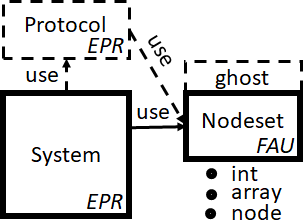
\includegraphics[scale=0.4]{fig-toy-modules-3}
%\end{minipage}
\caption{\label{fig:toy-c}Toy Leader Election pseudocode.}
\end{figure}


\subsection{Approach}
In this paper we present a verification methodology based on decidable
reasoning. We use it to develop and verify implementations of
distributed systems, whose performance is similar to other verified
implementations (e.g.~\cite{VerdiCPP}).
%, while reducing the human effort by an order of magnitude.
%obtained with tremendous human effort
%to efficient unverified implementations
%(e.g. \texttt{etcd}~\cite{etcd})
Rather than starting with an existing implementation (e.g., in C), we
define a simple imperative language which permits effective
(decidable) reasoning on one hand, and straightforward compilation
to efficient C++ code on the other hand.

%\paragraph{Modular proofs}
Our method leverages modularity in the assume-guarantee style for decidable reasoning,
%predictable automation,
by structuring the correctness proof such that different parts of the proof reason about
different aspects of the system, and at different abstraction levels, enabling each of them to
be carried out in (possibly different) decidable logics.
%Technically, this is achieved using the concept of \emph{modules} in an assume-guarantee style.
%Each module consists of procedures, pre/post-conditions and invariants, and is verified separately, while assuming the post-conditions and invariants guaranteed by other modules, in an assume-guarantee style.
The decomposition has two benefits. First, %the decomposition of the proof
it allows to reduce quantifier alternations, and eliminate bad quantification cycles. Second, it allows to check the verification conditions of each module using a different background theory (or none). % abstraction.
%n appropriate theory abstraction, making each check decidable.

\commentout{

\paragraph{Reasoning with decidable logics}
We use decidable logics to specify and check the correctness proof. This has the advantage of providing \emph{predictable} automation. In particular, when the proof is incorrect, we are able to present the user with counterexamples that make the failure visible to the user, assisting the user in fixing the proof.
However, decidable logics are rather limited. We use modularity to overcome their limitations.

\paragraph{Modular proofs}
Our method leverages modularity for decidable reasoning,
%predictable automation,
by structuring the correctness proof such that different parts of the proof are carried out in different
decidable logics. In this way, we break the undecidable problem of checking the verification conditions of the overall system
into several decidable sub-problems, each of which reasons about
different aspects of the system, and at different abstraction levels.
%
%
%Our method breaks the undecidable problem of verification
%into several decidable sub-problems, each of which reasons about
%different aspects of the system, and at different abstraction levels.
%%
%\TODO{merge with previous paragraph (repetition)} In this work we
%leverage modularity for predictable automation, by structuring the
%proof such that different parts of the proof are carried out in different
%decidable logics.
%
This is achieved using the concept of \emph{modules}.
Each module consists of procedures, pre/post-conditions and invariants, and forms a proof unit.
%Modules may be verified separately, while assuming the post-conditions and invariants guaranteed by other modules, in an assume-guarantee style. Their composition can be verified based on several proof rules.

This has two benefits. First, the decomposition of the proof allows to reduce quantifier alternations, and eliminate bad quantification cycles. Second, it allows to check the verification conditions of each module using a different theory abstraction.
%n appropriate theory abstraction, making each check decidable.
This is done by treating some symbols as interpreted inside the module that defines them, but (optionally) treating them as uninterpreted in other modules.
In this way, we decompose the proof into verification conditions that are checked independently, in different theories, and with different (stratified) quantifier alternations.
As a result, the modular proof may be checked in decidable fragments, even though the global proof would contain multiple theories and non-stratified quantifier alternations.

}
\commentout{
This is achieved by two key ideas: modularity and separate theories.

First, we decompose the verification problem into multiple subproblems, each concerning a different aspect of the proof, using the concept of \emph{modules}.
Each module consists of procedures, pre/post-conditions and invariants. The module can be understood as a lemma, which states that as long as the module's procedures are called in accordance with its preconditions, they will satisfy their postconditions, and the module invariant will be maintained.
This lemma can be used by other modules, by relying on postconditions and invariants, without inlining the proof.
Furthermore, each module (lemma) is proven separately, by checking its verification conditions.
This follows the assume-guarantee paradigm.
%This modular structure gives rise to multiple verification conditions.

The second key enabler of decidability is separation of theories. Namely, we allow to check each verification condition using an appropriate theory abstraction, making each check decidable.
This is done by treating some symbols as interpreted inside the module that defines them, but (optionally) treating them as uninterpreted in other modules.
%Furthermore, each VC can have different quantifier alternation structure, allowing each VC to be stratified, even though the global proof is not stratified.

By combining these two ideas, we decompose the proof into verification conditions that are checked independently, in different theories, and with different (stratified) quantifier alternations.
As a result, the modular proof may be checked in decidable fragments, even though the global proof would contain multiple theories and non-stratified quantifier alternations.
}

\commentout{
%\paragraph{Obtaining modular proofs of distributed systems}
\paragraph{Patterns for obtaining modular proofs}
We identify two patterns that capture common programming languages practices, and allow for a natural decidable decomposition:
%of the proof into a modular proof:
1)~Data structures
with first-order interfaces, and 2)~Protocol designs as lemmas for
proving the implementation.
We used these patterns to construct modular proofs for our examples. % enabled decidable reasoning in our examples.

\para{Data structures with first-order interfaces}
Efficient implementations deploy concrete primitive types (e.g.,
integers), which call for using theories (e.g., arithmetic) to reason about them.
Also, when it comes to distributed systems, the code of a process may be run by any number of nodes.
It is therefore natural to reason about such systems
%model unbounded (distributed) systems
in first-order logic, using quantifiers over unbounded domains (e.g., the set of nodes) and uninterpreted functions.
However, the combination of quantifiers, uninterpreted functions and,
e.g., arithmetic, often leads to undecidability. Encapsulating
primitive types in a pure (uninterpreted) first-order logic interface
decomposes the verification problem into the problem of reasoning in
uninterpreted first-order logic, where the primitive types are opaque
and only their interface is used, and reasoning about the low-level
implementation, showing that it satisfies its interface, which can be
done in decidable %(quantifier-free)
interpreted theories.

\para{Protocol designs as lemmas for proving the implementation}
Data structures with first-order interfaces simplify reasoning, but in
general, do not suffice for verifying interesting distributed systems
in decidable logics. The reason for this is that even the first-order
reasoning problem is undecidable, since proofs of complex systems
require quantifier alternation, which leads to
undecidability. Fortunately, distributed systems are constructed in an
evolutionary process starting with a protocol design, and then
gradually developing an efficient implementation, guided by the
protocol design. In this paper, we exploit this idea in a novel way,
by capturing the design and its correctness in a ghost object, which
is verified separately and serves as a lemma for proving the implementation. This provides a
natural way to further decompose the verification problem into
sub-problems, where each sub-problem usually contains fewer quantifier
alternations. In our limited experience, this usually results in each
problem becoming decidable, i.e., contain only stratified (acyclic)
quantifier alternations.

}

\commentout{
Data structures with first-order interfaces are a way to separate
reasoning about theories (e.g., arithmetic) from reasoning with
quantified first-order logic. We do this by encapsulating data
structures in a pure (uninterpreted) first order logic
specification. Each data structure is decomposed into an interface and
a corresponding implementation. The implementation is verified to
satisfy the interface using decidable (interpreted) theories capturing
features of the implementation. Properties of the implementation are
specified in pure first-order logic in order to be used in the proofs
of code using the data structure. These proofs rely solely on the
interface and result in verification conditions in quantified
uninterpreted first order logic. In this way we manage to eliminate
the need to combine quantifiers with interpreted theories. Secondly,
we decompose to reduce the reasoning over first-order quantifiers to
decidable checks, we use ghost objects to encapsulate pieces of proofs
in lemmas. Breaking a global proof into objects allows a proof
structure in which each object results in verification conditions in
first-order logic with stratified quantifier alternation, which
ensures decidability. A particularly useful way ghost objects are used
is as a way to separate the protocol design by abstracting some
implementation details, and then using the correctness of the design
as a lemma for proving the implementation correct.
}


%\subsection{Verification Friendly Modular Implementation}
\subsection{Modular Formulation}

% Modules used ...
% Modular...
%\TODO{add figure with modules}

We illustrate our methodology on the Toy Leader Election example, to verify that at most one
leader is elected using \emph{decidable} reasoning.
Our formulation of the system consists of three \emph{modules}: $\mtoyprotocol$, $\mtoysystem$, and $\mnodeset$.
The interplay between the modules and the decidable fragments in which they are verified are depicted in \Cref{fig:modules} (the fragments are defined in \Cref{sec:prelim}); their code is listed in \Cref{fig:toyprotocol,fig:toysystem,fig:nodeset}.
The code is written in {\bf M}odular {\bf D}ecidable {\bf L}anguage (\Lang) ---
an illustrative programming language enabling modular decidable verification.
% and implementation of distributed systems.

Each module should be viewed as a proof unit, which consists of
\begin{inparaenum}[(1)]
\item declarations and definitions of types and state components, which may be interpreted using \keyword{interpret} declarations,
\item declarations of other modules and their invariants that are used by the module, specified by the \keyword{uses} clause,
\item a module invariant $\modinvar$, given by all \keyword{invariant} declarations in the module,
\item procedures with pre-post specifications, specified by \keyword{requires} and \keyword{ensures} declarations (an
unspecified condition is $\true$ by default), and
\item declaration of the module's initial state, either with \keyword{init} declarations or with an $\pinit()$ procedure.
\end{inparaenum}
Intuitively, a module is correct if all its procedures satisfy their pre/post specification, and also maintain the module invariant,
assuming that the used modules are themselves correct.
The key property of the modular formulation is that verification conditions generated for each module fall into decidable fragments (see \Cref{subsec:overview:decidable}), which allows predictable automation.
%\oded{Please check last sentence}
%We note that our methodology is the first to employ decidable logics
%for reasoning all the way from protocol design to protocol
%implementation.


\commentout{
We illustrate our methodology on %a system that implements the simple leader election protocol.
the simple leader election example.
In order to facilitate \emph{decidable} reasoning for implementing and verifying the safety of this system, i.e., that at most one
leader is elected, we apply modular reasoning using the two patterns discussed above.
To that end, our formulation of the system consists of three \emph{modules}. %, where each module should be viewed as a proof unit.
The interplay between these modules and the fragments in which each of them is verified are depicted in \Cref{fig:modules}; their code is listed in \Cref{fig:toyprotocol,fig:toysystem,fig:nodeset}.
The code is written in the {\bf M}odular {\bf D}ecidable {\bf L}anguage (\Lang) ---
a language for modular decidable verification and implementation of distributed systems.
In our evaluation, we simulate {\Lang} using the Ivy language and system~\cite{Ivy,ken_fmcad16}.
}

\commentout{
\begin{figure}
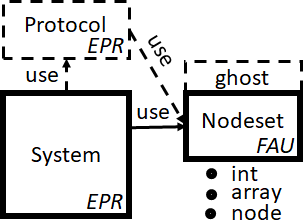
\includegraphics[scale=0.5]{fig-toy-modules-3}
\caption{Modules and built-in types used for verifying the toy example. Ghost modules (or parts of modules) are depicted using dashed lines.
Each module is annotated with the decidable fragment in which it was verified. \label{fig:modules}}
\end{figure}
}


\begin{SCfigure}
\caption{Modules and built-in types used for verifying the toy example. Dashed box denotes a ghost module.
Each module is annotated with the decidable fragment in which it is verified. \label{fig:modules}}
    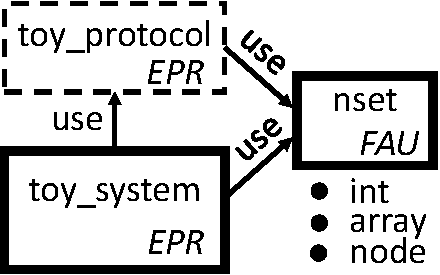
\includegraphics[scale=0.6]{modules-fig-trim}
\end{SCfigure}

We elaborate on the modules of the Toy Leader Election example in \Cref{sec:toyprotocol,sec:toysystem,sec:nodeset}.
Roughly speaking:

%In the example, t
(i) The {\mnodeset} module defines (and verifies) a data type which encapsulates sets of nodes under a first-order interface,
and hides the low-level implementation.
This allows other modules to treat sets of nodes as an opaque type, relying only on the first-order interface, so their verification can be carried out in uninterpreted first-order logic.
Verifying that the $\mnodeset$ module satisfies its interface is carried out in a suitable theory.
The first-order interface includes a predicate that tests if a set of nodes forms a majority,
along with the property that any two majorities intersect, which is crucial for the proof of the protocol.

(ii) The {\mtoyprotocol} module defines (and verifies) an abstract model of the protocol, eliding some of the
implementation details.
This is in line with the common practice of developing a system in an evolutionary process:
starting with a design, and then gradually developing an efficient implementation.
Here this practice serves a different purpose; namely, the {\mtoyprotocol} captures the protocol design and its correctness in a ghost object,
which is verified separately and serves as a lemma for proving the implementation.
This provides a natural way to decompose the verification problem,
and as we shall see, to avoid quantifier alternation cycles.

(iii) The {\mtoysystem} module specifies (and verifies) the system implementation,
using both the data type defined by $\mnodeset$ (relying on its first-order specification) and the
abstract protocol defined by $\mtoyprotocol$ (as ghost code) to obtain a verified executable implementation.

% We elaborate on these modules below.

\subsubsection{Abstract Protocol Module}
\label{sec:toyprotocol}
%\subsection{Protocol Designs as Lemmas for Proving Implementations}

\begin{figure}
\begin{lstlisting}[
    %frame=single,
    basicstyle=\scriptsize,%\footnotesize,
    keepspaces=true,
    numbers=left,
    %numbersep=1em,
    xleftmargin=2em,
    numberstyle=\tiny,
    emph={
      %% assert, assume,
      %% if, then else,
      %% while, do,
      %% sort, relation, function,
      %% axiom,
      %% insert,
    },
    emphstyle={\bfseries},
    mathescape=true,
  ]
ghost module $\mtoyprotocol$ uses $\mnodeset$, $\mnodeset.\iintersect$ { $\label{line:protocol:uses}$
  relation $\rvoted$ : $\snode,\snode$
  relation $\risleader$ : $\snode$
  variable $\rquorum$ : $\snodeset$
  init $\forall n_1,n_2. \; \neg\rvoted(n_1,n_2)$
  init $\forall n. \neg\risleader(n)$
  invariant $\ioneleader$ = $\forall n_1, n_2. \; \risleader(n_1) \land \risleader(n_2) \to n_1 = n_2 \label{line:toyprotocol-inv-1}$
  invariant $\forall n,n_1,n_2. \; \rvoted(n,n_1) \land \rvoted(n,n_2) \to n_1 = n_2 \label{line:toyprotocol-inv-2}$
  invariant $\forall n : \snode. \; \risleader(n) \to \big( \mnodeset.\rmajority(\rquorum) \, \land \label{line:toyprotocol-inv-3}$
                                     $\forall n':\snode. \; \mnodeset.\rmember(n' , \rquorum) \to \rvoted(n', n)\big)$
  procedure $\pvote(\text{v} : \snode ,\, \text{n} : \snode)$ {
    requires $\forall n'. \neg\rvoted(\text{v},n')$
    $\rvoted(\text{v}, \text{n})$ := true
  }
  procedure $\pbecomeleader(\text{n} : \snode ,\, \text{s} : \snodeset)$ {$\label{line:toyprotocol-becomeleader}$
    requires $\mnodeset.\rmajority(\text{s}) \, \land$ $\forall n':\snode. \; \mnodeset.\rmember(n' , \text{s}) \to \rvoted(n', n)\label{line:toyprotocol-becomeleader-pre}$
    $\risleader(\text{n})$ := true $\label{line:toyprotocol-becomeleader-assign-1}$
    $\rquorum$ := s $\label{line:toyprotocol-becomeleader-assign-2}$
  }
}
\end{lstlisting}
\caption{\label{fig:toyprotocol}Protocol module for Toy Leader Election.}
\end{figure}


%\TODO{add line references} \TODO{use different notation for named invariant}
\Cref{fig:toyprotocol} lists the module that formalizes the
abstract leader election protocol.
This is a ghost module, which is only used for the sake of the proof.
%, presented in {\Lang}a simplified form of the Ivy language \TODO{name the language. SH: I don't think it is necessary}.
The module contains two mutable relations that define its state:
$\rvoted(n_1,n_2)$ captures the fact that $n_1$ voted for $n_2$, and
$\risleader(n)$ means node $n$ is an elected leader. The initial state
of the module specifies that both relations are empty. The state also
includes a variable $\rquorum$, that remembers the last voting
majority observed. The abstract protocol provides a global invariant
(denoted by \keyword{invariant}), which states that there is at most
one leader. This is similar to a class invariant / object invariant in
modular reasoning. Next, the module contains a proof that all of its
reachable states satisfy the global invariant, by an inductive
invariant. When proving this module, the majority intersection
invariant of the $\mnodeset$ module is used, as indicated by the
\keyword{uses} clause in \cref{line:protocol:uses}.

The module also provides two procedures that define the abstract
protocol steps. Each procedure specifies a pre condition.
%, denoted by the \keyword{requires} and \keyword{ensures} keywords (an
%unspecified condition is $\true$ by default).
The $\pvote(n_1,n_2)$
procedure models a vote by $n_1$ for $n_2$, and its precondition is
that node $n_1$ has not yet voted. The $\pbecomeleader(n,s)$ procedure
models the election of $n$ as a leader, and its precondition requires
that all nodes in $s$ voted for $n$, and that $s$ is a majority.
%
Note that this module is abstract in the sense that it abstracts network communication and uses a global view of the system. In particular, the $\pbecomeleader$ does not specify how a node learns that it received a majority of votes.
%\TODO{Indeed, it is a \keyword{ghost} module, which is only used for the sake of the proof.}
%thus avoiding the local bookkeeping.

\commentout{
nodes have a global view of the system (e.g., via the $\rvoted$ relation), and may directly access the local state of other nodes, without exchanging messages. Clearly, such a module cannot be implemented in a distributed setting. Indeed, it is a \keyword{ghost} module, which is only used for the sake of the proof.
\TODO{emphasize in what ways it is abstract: it has global view. No messages, etc.}
}

\commentout{
%%% MOVED
During modular verification, this module will result in verification
conditions (VC's) that check: 1) $\INV$ --- the provided inductive
invariant combined with the global guarantee, holds at any initial
state, and 2) that the execution of a procedure starting from states
that satisfy $\INV$ and the precondition result in states that satisfy
$\INV$ and the postcondition. The VC's will also assume the
{\iintersect} guarantee of the nodeset datatype. Fig X lists
these verification conditions. These verification conditions contain
$\forall\exists$ quantifier alternation from nodeset to node, but this
is stratified and therefore decidable to check.

\TODO{add figure with VC's}
}

\subsubsection{Concrete Implementation Module}
\label{sec:toysystem}

\begin{figure}
\begin{lstlisting}[
    %frame=single,
    basicstyle=\scriptsize,%\footnotesize,
    keepspaces=true,
    numbers=left,
    %numbersep=1em,
    xleftmargin=2em,
    numberstyle=\tiny,
    emph={
      %% assert, assume,
      %% if, then else,
      %% while, do,
      %% sort, relation, function,
      %% axiom,
      %% insert,
    },
    emphstyle={\bfseries},
    mathescape=true,
  ]
system module $\mtoysystem$ uses $\mnodeset$, $\mtoyprotocol$, $\mtoyprotocol.\ioneleader$ { $\label{line:toysystem-uses}$
  message $\msgrequestvote$ : $\snode$  $\label{line:system:msg-def1}$
  message $\msgvote$ : $\snode, \snode$ $\label{line:system:msg-def2}$
  message $\msgleader$ : $\snode$ $\label{line:system:msg-def3}$
  // $\emph{spec: at most one node sends \msgleader}:$
  invariant $\isafe$ = $\forall n_1, n_2. \; \msgleader(n_1) \land \msgleader(n_2) \to n_1 = n_2$ $\label{line:system-guarantee}$

  relation $\ralreadyvoted$ : $\snode$ $\label{line:system-begin-node}$
  function $\rvoters$ : $\snode \to \snodeset$
  procedure $\pinit(\text{self}:\snode)$ {
    $\ralreadyvoted(\text{self})$ := false
    $\rvoters(\text{self})$ := $\mnodeset.\pemptyset()$
  }
  procedure $\prequestvote(\text{self}:\snode)$ {
    send $\msgrequestvote(\text{self})$
  }
  procedure $\pcastvote(\text{self}:\snode ,\, \text{n}:\snode)$ handles $\msgrequestvote(\text{n})$ {
    if $\neg\ralreadyvoted(\text{self})$ {
      $\ralreadyvoted(\text{self})$ := true
      send $\msgvote(\text{self}, \text{n})$
      $\mtoyprotocol.\pvote(\text{self}, \text{n})$ $\label{line:system:ghost-2}$
    }
  }
  procedure $\preceivevote(\text{self}:\snode, \text{n}:\snode)$ handles $\msgvote(\text{n},\text{self})$ {
    $\rvoters(\text{self})$ := $\mnodeset.\padd(\rvoters(\text{self}), \text{n})$
    if $\mnodeset.\rmajority(\rvoters(\text{self}))$ { $\label{line:system:majority}$
      send $\msgleader(\text{self})$
      $\mtoyprotocol.\pbecomeleader(\text{self},\rvoters(\text{self}))$ $\label{line:system:ghost-3}$
    }
  } $\label{line:system-end-node}$
  // $\emph{inductive invariant for the proof:}$
  invariant $\forall n_1,n_2. \; \mtoyprotocol.\rvoted(n_1,n_2) \leftrightarrow \msgvote(n_1,n_2)$ $\label{line:system:inv-1}$
  invariant $\forall n_1,n_2. \, \mnodeset.\rmember(n_1,\!\rvoters(n_2)) \! \to \! \mtoyprotocol.\rvoted(n_1,\!n_2)$ $\label{line:system:inv-2}$
  invariant $\forall n. \; \msgleader(n) \leftrightarrow \mtoyprotocol.\risleader(n)$ $\label{line:system:inv-3}$
  invariant $\forall n_1,n_2. \; \neg \ralreadyvoted(n_1) \to \neg \mtoyprotocol.\rvoted(n_1,n_2)$ $\label{line:system:inv-4}$
  open $\mtoyprotocol$ $\label{line:system:open}$
}
\end{lstlisting}
\caption{\label{fig:toysystem}System module for Toy Leader Election. }
\end{figure}


\Cref{fig:toysystem} lists the concrete system implementation.  We
consider systems in which a finite (but unbounded) set of nodes run
the same code, and exchange messages. For simplicity, we assume all
messages are broadcast to all nodes. Our network model also allows
message dropping, duplication and reordering. To define the system
implementation, we first define the message
types. \Cref{line:system:msg-def1,line:system:msg-def2,line:system:msg-def3}
define three message types: {\msgrequestvote} that a node uses to
propose itself as a leader, {\msgvote} that a node sends to vote for a
candidate, and {\msgleader} that a node uses to announce it is elected
as the leader. The first field of each message is its source
node.
%\ken{Following two sentences added in response to shepherd comment 3}
The invariant on \cref{line:system-guarantee} specifies the desired specification, i.e., that only
one node ever issues a {\msgleader}
message. This is the ultimate guarantee provided by the implementation,
and it is the only line of trusted specification in the
example. Namely, one has to trust that this invariant captures the intended property (e.g., by careful inspection),
but the fact that the implementation maintains it is mechanically verified.
%\sharon{I don't understand this sentence. In what sense is it trusted code? it is the invariant??}
%\oded{It's supposed to answer the reviewer's question. This line is trusted in the sense that if we wrote it wrong (suppose we had a typo that makes it equivalent to true), Ivy wouldn't catch us. Any error in any other part of the code would be caught. Maybe we can think of a better wording}
%\sharon{I think we should remove it. It is as trusted as any other invariants: all of them are verified. What is not verified is whether this logical formula captures the intent of the user, just like the code may be not exactly what the user wanted. We can just say "Unlike the other annotations, which are internal to the proof, this invariant defines the specification that is being verified (and is therefore of special interest to the user)." }
The declarations are followed by the code to be run on each node. This
code (lines \ref{line:system-begin-node} to
\ref{line:system-end-node}) defines the local state of each node, as
well as procedures that can be executed in response to client
requests, or procedures that are message handlers (specified by the
\keyword{handles} declaration), and executed upon receiving a message
from the network. The state components are defined as functions (or
relations) whose first argument is a node, so that $f(n)$ denotes the
local state of node $n$.  Similarly, all procedures receive as their
first argument the {\self} identifier of the node that runs them.
Since the system module is going to be compiled into an executable
code that runs on each node, we syntactically enforce that each node
may only access and modify its own local state.
% (via the {\self} identifier).

We note that the $\mtoysystem$ module makes use of the $\mnodeset$
module to maintain sets of voters, and uses a majority test
(\cref{line:system:majority}). It also makes calls into the ghost
module $\mtoyprotocol$
(\cref{line:system:ghost-2,line:system:ghost-3}). This allows to
establish an invariant that relates the state of the concrete module
and the abstract module
(\cref{line:system:inv-1,line:system:inv-2,line:system:inv-3,line:system:inv-4}),
and use the proven invariant of the abstract module as a lemma for
proving the concrete implementation. This is indicated by the
\keyword{uses} clause, which declares use of the
$\mtoyprotocol.\ioneleader$ invariant (\cref{line:toysystem-uses}).

%\subsubsection{Data Structures with First-Order Interfaces}
\subsubsection{Node Set Module}
\label{sec:nodeset}

\begin{figure}
\begin{lstlisting}[
    %frame=single,
    basicstyle=\scriptsize,%\footnotesize,
    keepspaces=true,
    numbers=left,
    %numbersep=1em,
    xleftmargin=2em,
    numberstyle=\tiny,
    emph={
      %% assert, assume,
      %% if, then else,
      %% while, do,
      %% sort, relation, function,
      %% axiom,
      %% insert,
    },
    emphstyle={\bfseries},
    mathescape=true,
  ]
module $\mnodeset$ {
  type t
  relation $\rmember$ : $\snode,\text{t}$
  relation $\rmajority$ : t
  function $\risize$ : t $ \to \sint$

  interpret t as array<$\sint$,$\snode$> $\label{line:nodeset-t}$
  interpret $\rmember(n,s)$ as $\exists i. 0 \leq i < \rlen(s) \land \rvalue(s,i,n)$ $\label{line:nodeset-member}$
  interpret $\rmajority(s)$ as $\risize(s) + \risize(s) > \risize(\rallnodes)$ $\label{line:nodeset-majority}$

  invariant $\iintersect$ = $\forall s_1, s_2. \; \rmajority(s_1) \land \rmajority(s_2) \,\to$ $\label{line:nodeset-intersect}$
                            $\exists n. \; \rmember(n, s_1) \land \rmember(n, s_2)$

  procedure $\pemptyset()$ returns s:t {
    ensures $\forall n. \; \neg\rmember(n,\text{s})$
    s := array.empty()
  }
  procedure $\padd(\text{s}_1 : \text{t} ,\, \text{n} : \snode)$ returns $\text{s}_2 : \text{t}$ {
    ensures $\forall n'. \; \rmember(n', \text{s}_2) \leftrightarrow (\rmember(n', \text{s}_1) \lor n' = n)$
    if $\rmember(\text{n}, \text{s}_1)$ then { $\text{s}_2$ := $\text{s}_1$ } else { $\text{s}_2$ := array.append($\text{s}_1$, n) } $\label{line:nodeset-append}$
  }
  procedure $\pinit()$ {
    $\risize$ := $\lambda x. 0$;
    for $0 \leq i < \rlen(\rallnodes)$ {
      invariant $\forall s_1,s_2. (\forall n. \neg (\rmember(n,s_1) \land \rmember(n, s_2))) \, \to$ $\label{line:nodeset-inv}$
          $\risize(s_1) + \risize(s_2) \leq \risize(\rallnodes)$
      $\risize$ := $\lambda x. \big( (\risize(x) + 1)$ if $\rmember(\text{array.get}(\rallnodes,i),x)$ else $\risize(x)\big)$ $\label{line:nodeset-lambda}$
    }
  }
}
\end{lstlisting}
\caption{\label{fig:nodeset}The $\mnodeset$ module for node sets, proving the majority intersection property.}
\end{figure}

\commentout{
  ghost relation $\rreachedset$ : t
  interpret t as array<$\sint$,$\snode$> with $\rreachedset$
  interpret $\rreachedset(s)$ as $\rlen(s) = \risize(s)$

  invariant $0 \leq i \leq \rlen(\rallnodes)$

}



\Cref{fig:nodeset} lists the code for the $\mnodeset$ module. This
module defines a data structure for storing sets of nodes, with
operations for adding to a set and testing whether a set is a
majority. To do so, it defines a type t, whose internal interpretation is \Lang's
built-in array, as declared in \cref{line:nodeset-t}.
%The implementation uses \Lang's built-in arrays as a
%naive implementation for sets.
Sets are created using the $\pemptyset$ and $\padd$ procedures, which
provide a naive implementation of a set, stored as an array of its
elements.  The module defines the $\rmember$ relation, and provides it
with an interpretation via an \keyword{interpret} declaration in
\cref{line:nodeset-member}. As we shall see, this definition creates
an executable membership test that is translated to a loop that scans
the array.

Most importantly for verifying the leader election modules, the
$\mnodeset$ module provides the interpreted $\rmajority$ predicate,
with the key property that any two majorities intersect. This is
stated by the $\iintersect$ invariant (\cref{line:nodeset-intersect}).
Intuitively, a set is a majority if its cardinality is more than half
the total number of nodes.  In \Cref{fig:nodeset}, the $\rmajority$
predicate is interpreted using the $\risize$ function to compute the
cardinality of a set of nodes, and the built-in value $\rallnodes$,
which is an array with the special semantics that it contains all
nodes.  The $\risize$ function computes the cardinality of a set of
nodes, and it is constructed in the $\pinit()$ procedure of the
$\mnodeset$ module in a way that establishes the majority intersection
property. The proof is by induction, manifested in the loop invariant
in \cref{line:nodeset-inv}.

We note that the loop in $\pinit()$ constructs $\risize$ via a nesting
of $N$ function closures (where $N$ is the number of nodes). This
definition of $\risize$ allows an easy proof of the majority
intersection property (the $\lambda$ at \cref{line:nodeset-lambda} is eliminated from verification conditions by $\beta$-reduction, resulting in first-order formulas; see \Cref{sec:extensions}). A more efficient implementation uses $\rlen$
(underlying array length) instead of $\risize$ to determine if a set
is a majority. This implementation is also provable in our system,
%\sharon{ (and was used in our realistic examples)},
but requires additional inductive invariants
%(and ghost state)
to prove that $\risize$ and $\rlen$ coincide, and we do not present it
here in the interest of simplicity.

\commentout{
The key argument for the proof of $\iintersect$ is that: $\card{X} + \card{Y} \leq
\card{Z}$ whenever $X$ and $Y$ are disjoint subsets of $Z$. This
invariant is most easily proven by induction over the size of the sets
if we define cardinalities of finite sets by induction over the elements.
%
Interestingly, we manage to convert this induction to induction over time.
%A simple proof of
%this property is done by induction over the size of the sets. Interestingly,
Namely, we encode this induction via ghost code in the $\pemptyset$ and $\padd$
procedures. Together with the inductive invariant provided in
\cref{...}, this ghost code allows to prove that any two majorities
intersect. To formalize the induction via ghost code, the module
includes two ghost relations, $\rreachedset$ (which represents the ``reached'' sets) and $\rreachednode$ (which represents the ``reached'' nodes), as
well as a ghost, inductively-defined, size function $\risize$, which represents the cardinality of the reached sets, restricted to the reached nodes. As such, the $\risize$ function is updated whenever a new node is reached.
%The key
%inductive invariant for the proof is that: \sharon{changed $\card{..}$ to $\risize$. Is it correct?}
%$\risize(X) + \risize(Y) \leq
%\risize(Z)$ whenever $X$ and $Y$ are disjoint subsets of $Z$. This
%invariant is most easily proven if we define cardinalities of finite sets by induction over the elements.
%This is captured by
%$\risize$.
However, for an efficient implementation, we wish to use
the length of the underlying array to obtain the cardinality of the
set, rather than using an inductive definition. This is obtained by
proving that $\risize$ coincides with the length of an array. Finally,
to determine whether a set is a majority, its size must be compared to
the size of the set of all nodes. To achieve this, the initialization
code of the $\mnodeset$ module constructs a $\mnodeset.t$ element with
all nodes, using \Lang's provided $\snode.\text{all}$ construct, which
is known to contain all nodes.
}

\commentout{
The proof of
this property is done by induction. Interestingly, we encode this
induction via ghost code in the $\pemptyset$ and $\padd$
procedures. Together with the inductive invariant provided in
\cref{...}, this ghost code allows to prove that any two majorities
intersect. To formalize the induction via ghost code, the module
includes two ghost relation $\rreachedset$ and $\rreachednode$, as
well as a ghost, inductively-defined, size function $\risize$. The key
inductive invariant for the proof is that: $\card{X} + \card{Y} \leq
\card{Z}$ whenever $X$ and $Y$ are disjoint subsets of $Z$. This
invariant is most easily proven if we define cardinalities of finite
sets by induction over the elements. This is captured by
$\risize$. However, for an efficient implementation, we wish to use
the length of the underlying array to obtain the cardinality of the
set, rather than using an inductive definition. This is obtained by
proving that $\risize$ coincides with the length of an array. Finally,
to determine whether a set is a majority, its size must be compared to
the size of the set of all nodes. To achieve this, the initialization
code of the $\mnodeset$ module constructs a $\mnodeset.t$ element with
all nodes, using \Lang's provided $\snode.\text{all}$ construct, which
is known to contain all nodes.
}

\commentout{
Explain nodeset module, and say that \texttt{nodeset\_aux} is
explained in the paper, and is used to prove the majority intersection
property. Explain the \texttt{INTERPRET} clauses, and the fact that
they allow both code extraction and verification (by substitution).
}

\subsection{Modular Verification in Decidable Fragments} \label{subsec:overview:decidable}

\commentout{
Recall that in order to verify safety of the system, i.e., that at
most one leader is elected, the main safety property of the
implementation module,

We now explain how the modular formulation can be verified using
decidable logics, resulting in a proof
}

\commentout{
In order to verify the safety of the system, i.e., that at most one
leader is elected, we apply modular verification. Recall that each
module contains a set of procedures, with pre and post conditions, and
an invariant $\INV$, given by the conjunction of all
\texttt{INVARIANT} declarations in the module. Each module may also
use invariants from other modules as assumptions, specified by
\texttt{USE} declarations.
}

\commentout{
\TODO{rethink this opening paragraph: we first give general explanations and only then become more example specific}
In the sequel, we explain the verification conditions generated for the toy consensus example, and the theories under which they are checked.
%Recall that each module forms a proof unit. In the sequel, we explain the verification conditions generated for each module, and the theories under which they are checked.
In particular, we show how modularity enables decidability. Specifically, in the example we use two decidable fragments of first-order logic: the effectively propositional (EPR) fragment~\cite{EPR} and the finite almost uninterpreted (FAU) fragment~\cite{ge2009complete}
%, and the almost uninterpreted fragment~\cite{ge2009complete}
(the precise definition of these fragments is not essential for understanding the rest of this section).
}

We now explain how verification conditions are generated for each module, and how they are checked under (possibly different) theories.
We use two decidable fragments: the effectively propositional (EPR) fragment~\cite{EPR} which allows stratified quantifier alternations,
and the finite almost uninterpreted (FAU) fragment~\cite{ge2009complete} which includes linear integer arithmetic in a restricted way.
%The precise definitions of these fragments are not essential for understanding the rest of this section.

\commentout{Breaking the proof into separate modules already plays a big role in the ability to obtain verification conditions that are decidable to check. However, this does not always suffice. We therefore explain how \emph{theories} may either be used to provide interpretations to the state elements of the module, or be abstracted to provide simpler verification conditions that fall into decidable fragments.
}

%\paragraph{Verification conditions}
\paragraph{Verification Condition Generation}
Recall that each module declares the modules and invariants it uses in the \keyword{uses} clause.
%This determines how modules are stacked together to result in a complete proof of the system.
Based on this, verification conditions are derived automatically.
%\ken{I replaced the discussion of VC generation here as I found the sentence too long and hard to follow.}
Each module must provide the following \emph{guarantees}:
\begin{inparaenum}[1)]
\item The module invariant, $\modinvar$, holds at any initial state.
\item Every procedure in the module establishes its postcondition and preserves the module invariant $\modinvar$, and
\item At each call site, the precondition of the called procedure is established.
\end{inparaenum}
Each module may rely upon the following \emph{assumptions}:
\begin{inparaenum}[1)]
\item Every called procedure establishes its postcondition and
\item Every used invariant of another module holds at all times.
\end{inparaenum}
The verification condition states that the assumptions imply the guarantees.

As an example, the verification condition generated for the $\pbecomeleader$ procedure (\Cref{fig:toyprotocol} \cref{line:toyprotocol-becomeleader}) is:
%\begin{small}
\begin{align*}
&
\big( \modinvar_\mtoyprotocol \land
\modinvar_{\mnodeset.\iintersect} \, \land \\
&
\left( \rmajority(s) \land \forall n'. \, \rmember(n' , s) \to \rvoted(n', n) \right)
\big) \to \\
&
\modinvar_\mtoyprotocol \left[\left(\risleader(x) \lor x=n\right) /~ \risleader(x) \,,\,  s ~/~ \rquorum \right]
\end{align*}
%\end{small}
where $\modinvar_\mtoyprotocol$ is given by \Cref{fig:toyprotocol}
\cref{line:toyprotocol-inv-1,line:toyprotocol-inv-2,line:toyprotocol-inv-3} and \linebreak $\modinvar_{\mnodeset.\iintersect}$
is given by \Cref{fig:nodeset} \cref{line:nodeset-intersect}.  The
latter is used because it appears in the \keyword{uses} clause of the
$\mtoyprotocol$ module.  The verification condition also includes the
procedure precondition taken from \Cref{fig:toyprotocol}
\cref{line:toyprotocol-becomeleader-pre}, and checks that assuming the
invariants and the precondition, the invariant
$\modinvar_\mtoyprotocol$ is preserved by the procedure (the
substitutions reflect the assignments of
\cref{line:toyprotocol-becomeleader-assign-1,line:toyprotocol-becomeleader-assign-2}).

Optionally, calls to procedures may be inlined (i.e., replaced by the
procedure body), and we may take the initial condition of another
module as an assumption. If we use a module in this way, we say the
module is \emph{opened}. As an example, ghost module $\mtoyprotocol$ is
opened in the verification of
$\mtoysystem$ (\Cref{fig:toysystem}, \cref{line:system:open}).  This
allows us to establish easily an invariant relating the states of the
two modules.
%
When composing modules, there are additional conditions required for
soundness (e.g., that modules do not interfere), which are described
in \Cref{sec:modular}.
%

\commentout{
\TODO{remove? rephrase? }
Fig X lists the verification conditions of the abstract protocol module. These verification conditions contain
$\forall\exists$ quantifier alternation from nodeset to node, but this
is stratified and therefore decidable to check.
Importantly, while the \texttt{pintersect} invariant of the nodeset datatype is used in the proof of the abstract protocol module, its proof is not.
Due to this division of the proof, the verification conditions remain decidable to check.
\TODO{can we be more specific and say that if we added one of the other invariants, we would get a cycle?}

\TODO{add figure with VC's}
}

%\paragraph{Verification in decidable fragments}
%\paragraph{Segregating theories}
%\paragraph{Using Theories}
\paragraph{Theory Abstractions}
%\TODO{better paragraph title?}
%Separating the modules (and their invariants) and breaking the proof into verification conditions for each procedure already plays a big role in the ability to obtain verification conditions that are decidable to check. However, this does not always suffice. Next, we explain how \emph{theories} may either be used to provide interpretations to the state elements of the module, or be abstracted to provide simpler verification conditions that fall into decidable fragments.

Recall that every module may include interpreted types (e.g., int, array)
as well as definitions via \keyword{interpret} declarations.
These allow the module to define its relevant \emph{theory}.
%, via the \texttt{INTERPRET} declarations.
A theory is a (possibly infinite) set of first-order formulas, which may either be given explicitly (e.g., the theory of total order), or by using a built-in theory (e.g., the theory of linear integer arithmetic).
The verification conditions of the module are checked with respect to the provided theory and definitions.
Symbols that are given no interpretation in the module are treated as uninterpreted,
which may be viewed as a form of abstraction.
%that simplifies the verification conditions and may turn them to decidable.
%is sometimes crucial for making the verification conditions decidable to check, as we demonstrate next.

For example, when checking the verification condition of the
$\pbecomeleader$ procedure given above, the $\rmajority$ and
$\rmember$ relations are treated as uninterpreted relations, and not
according to their definitions from \Cref{fig:nodeset}
\cref{line:nodeset-member,line:nodeset-majority}. In contrast, when
verifying the $\mnodeset$ module, these definitions are used as part
of a background theory, which also includes linear integer arithmetic.

%\paragraph{Putting it all together: decidable checks used in the leader election example}
%\paragraph{Decidable verification of the leader election example}
\paragraph{Decidable Decomposition of Toy Leader Election}
%Every module also defines its relevant \emph{theory}, via the
%\texttt{INTERPRET} declarations. A theory is a (possibly infinite) set
%of first-order formulas.

For the whole picture of our example, observe that the {\mnodeset} module uses the $\sint$ type, which introduces the theory of linear integer arithmetic.
Furthermore, its {\iintersect} invariant introduces quantifier alternation from $\snodeset$ to $\snode$.
The function $\rvoters$ of the {\mtoysystem} module introduces a dependency in the opposite direction, as it is a function from $\snode$ to $\snodeset$.
%An invariant of the {\mtoyprotocol} module, which specifies the main safety property of the protocol, introduces a quantifier alternation in the opposite direction: from $\snode$ to $\snodeset$.
As a result, had the $\mnodeset$ module and its invariants been inlined within the proof of {\mtoysystem}, they would have resulted in verification conditions that combine arithmetic, quantifier alternation cycles, and uninterpreted symbols, breaking decidability.

\begin{sloppypar}
In order to break the bad cycle, we do not directly use the {\iintersect} invariant of {\mnodeset} in {\mtoysystem}. Instead, our proof exploits the {\mtoyprotocol} module and its $\ioneleader$ invariant (which does not introduce dependency from $\snode$ to $\snodeset$). Namely, the invariant $\ioneleader$  is assumed when verifying {\mtoysystem}, and is verified separately as part of the {\mtoyprotocol} module (assuming the {\iintersect} invariant of {\mnodeset}).
In that way, $\mtoysystem$ only contains functions from $\snode$ to $\snodeset$, while $\mtoyprotocol$ only contains dependencies from $\snodeset$ to $\snode$, avoiding quantifier alternation cycles.
%its $\ioneleader$ invariant (which does not introduce dependency from $\snode$ to $\snodeset$) to verify {\mtoysystem}, and (2) verify the {\mtoyprotocol} module and its $\ioneleader$ invariant separately using the {\iintersect} invariant.
%Instead, our proof verifies each module separately, and
\end{sloppypar}

%Verifying each module separately also isolates the theory reasoning to the {\mnodeset} module. Indeed,
In terms of theories,
the {\mnodeset} module is verified when $\sint$ is interpreted using the theory of linear integer arithmetic,
and the {\tnodeset} type is interpreted as \sort{array$<$int,node$>$} from our built-in array theory (as explained in \Cref{sec:modular}, we encode arrays in FAU).
Moreover, the $\rmember$ and $\rmajority$ relations are interpreted by their definitions (\Cref{fig:nodeset} \cref{line:nodeset-member,line:nodeset-majority}).
The resulting verification conditions for this module are in FAU.
%
%When verifying the {\mtoyprotocol} and {\mtoysystem} modules, all sorts and relations (including $\rmember$ and $\rmajority$) are uninterpreted. {\mtoyprotocol} assumes the $\iintersect$ invariant of $\mnodeset$.
%{\mtoysystem} assumes the $\ioneleader$ invariant of {\mtoyprotocol} and inlines calls to its (ghost) procedures, while summarizing calls to procedures from {\mnodeset}. The resulting verification conditions are in EPR.
%
When verifying the {\mtoyprotocol} and {\mtoysystem} modules, sorts and relations (including $\rmember$ and $\rmajority$) are uninterpreted.
%{\mtoyprotocol} assumes the $\iintersect$ invariant of $\mnodeset$.
%{\mtoysystem} assumes the $\ioneleader$ invariant of {\mtoyprotocol}.
% and inlines calls to its (ghost) procedures, while summarizing calls to procedures from {\mnodeset}.
The resulting verification conditions are in EPR, as the quantifiers in each module are stratified.

We thus see that the separation between the three modules allows us to
obtain decidable verification conditions.

\commentout{
Verifying each module separately also isolates the reasoning about arithmetic to the {\mnodeset} module.
Namely, the {\mnodeset} module is verified when $\sint$ is interpreted using the theory of linear integer arithmetic, and when the $\rmember$ and $\rmajority$ relations are interpreted by their definitions (\cref{line:nodeset-member}-\cref{line:nodeset-member}). The verification conditions for this module are in FAU. %the finite almost uninterpreted fragment.
%, with (Skolem) functions from nodeset to node, which makes them decidable to check.
In the {\mtoyprotocol} and {\mtoysystem} modules, sorts and relations are uninterpreted, and the resulting verification conditions are in EPR.

When verifying the {\mtoysystem} module, all sorts remain
uninterpreted, calls to procedures from {\mnodeset} are
summarized, and calls to procedures from
{\mtoyprotocol} are inlined. Moreover, the
$\ioneleader$ invariant of {\mtoyprotocol} is assumed.
%Furthermore,
%{\mtoysystem} uses (via a \keyword{use} declaration) the
%unique leader invariant of {\mtoyprotocol}. This allows
%the invariant of {\mtoysystem} to relate the state of the
%concrete implementation to the (ghost) state of the abstract protocol,
%and to use the correctness of the abstract protocol as a lemma.
The verification conditions of this module are in EPR.

}

%
%\TODO{maybe rewrite the ``Next we elaborate on the verification of each module.'' that was here. For now it's in commentout.}
\commentout{
Next we elaborate on the verification of each module.

  %In our example, t
The {\mnodeset} module
interprets the type {\tnodeset} as \sort{array<int,node>},
which makes the theory of the {\mnodeset} module include the
theory of linear integer arithmetic, as well as provides access to the
\texttt{len} and \texttt{value} functions from the built-in array
module (as explained in \Cref{sec:modular}, we do not use the theory of
arrays, but use the more general finite essentially uninterpreted
fragment). The {\mnodeset} module also contains an
\keyword{interpret} declarations for $\rmember$ and $\rmajority$,
making relations interpreted, and adding the following formulas to its
theory:
%
\begin{small}
\begin{align*}
& \forall n,s. \; \rmember(n,s) \leftrightarrow \exists i. \; 0 \leq i < \rlen(s) \land \rvalue(s,i,n) \\
& \forall s. \; majority(s) \leftrightarrow \rlen(s) + \rlen(s) > \rlen(allnodes)
\end{align*}
\end{small}
%
Therefore, when verifying the {\mnodeset} module, these will be
added to the verification conditions as axioms. The resulting
verification conditions for the {\mnodeset} module are in the
finite essentially uninterpreted fragment, with (Skolem) functions from
nodeset to node, which makes them decidable to check.

When verifying the {\mtoyprotocol} module, the
$\rmember$ and $\rmajority$ relation are uninterpreted. However, since
{\mtoyprotocol} contains a \keyword{use} declaration for
{\iintersect}, it is verified under the assumption that
any two majorities intersect. In this module, all sorts are
uninterpreted, and verification conditions are in the effectively propositional fragment (EPR), with a (Skolem)
function from nodeset to node.

When verifying the {\mtoysystem} module, all sorts remain
uninterpreted, calls to procedures from {\mnodeset} are
summarized, and calls to procedures from
{\mtoyprotocol} are inlined. Furthermore,
{\mtoysystem} uses (via a \keyword{use} declaration) the
unique leader invariant of {\mtoyprotocol}. This allows
the invariant of {\mtoysystem} to relate the state of the
concrete implementation to the (ghost) state of the abstract protocol,
and to use the correctness of the abstract protocol as a lemma. The
verification conditions of this module are in EPR, with a function
from node to nodeset. This function results from the fact that the
local state of a node contains a nodeset that records its voters so
far. We thus see that the separation between the three modules allows
us to obtain decidable verification conditions. Without this
separation, the verification conditions would contain function cycles.
}

% \TODO{paragraph: Benefits of Decidability}


\commentout{
\paragraph{Modularity for Decidability}
To summarize, the key enabler for decidability in our approach is modularity. Our proofs exploit the modular structure in two ways.
First, the structure of modules decomposes the verification problem into multiple subproblems, each concerning a different aspect of the proof.
In this perspective, each module can be understood as a lemma, which states that as long as the module's procedures are called in accordance with its preconditions,
they will satisfy their postconditions, and the module invariant will be maintained.
This lemma can be used by other modules, by relying on postconditions and invariants, without inlining the proof.
Furthermore, each module (lemma) is proven separately, by checking its verification conditions.
%This modular structure gives rise to multiple verification conditions.
Second, each verification condition can be checked using an appropriate theory abstraction, making each VC check decidable.
This is done by treating some symbols as interpreted inside the module that defines them, but (optionally) treating them as uninterpreted in other modules.
%Furthermore, each VC can have different quantifier alternation structure, allowing each VC to be stratified, even though the global proof is not stratified.
By combining these two ideas, we decompose the proof into VC's that are checked independently, in different theories, and with different (stratified) quantifier alternations.
As a result, the modular proof may be checked in decidable fragments, even though the global proof would contain multiple theories and non-stratified quantifier alternations.
}

\commentout{
To summarize, our proofs are modular in three ways. First, we generate verification conditions for each procedure separately. This is standard in interprocedural analysis, but in our case it has an additional benefit of enabling the use of weaker logics for verification. Second, we use modules to group together invariants that are inductive as a set but not individually. In this way, they are all used together while carrying their proof, but each of them can be used separately as an assumption in other modules, without including the proof. Third, modules are also used as a mechanism to determine which theory to use for which part of the proof, by either providing interpretation to types and state elements or leaving them uninterpreted. The combination of these three ingredients makes it possible to verify complex systems using decidable verification conditions, despite the need to combine theories with non-trivial quantification (including quantifier alternations).
}

\commentout{
Breaking the proof into separate modules already plays a big role in the ability to obtain verification conditions that are decidable to check. However, this does not always suffice. We therefore explain how \emph{theories} may either be used to provide interpretations to the state elements of the module, or be abstracted to provide simpler verification conditions that fall into decidable fragments.
}

\commentout{
Each VC interpret, abstraction

2) the execution of every procedure in the module starting from states
that satisfy $\INV$, the assumption, and the precondition: a) result
in states that satisfy $\INV$ and the postcondition, and b) satisfy
the precondition of every called procedure (in any module).
%
When generating these VC's, calls to procedures are replaced by their
effect, summarized by their postcondition.


The VC's will also assume the \texttt{pintersect}
guarantee of the nodeset datatype. Fig X lists these verification
conditions. These verification conditions contain $\forall\exists$
quantifier alternation from nodeset to node, but this is stratified
and therefore decidable to check.


Explain that these modules are verified in three parts / isolates /
verification contexts. One for \texttt{toy\_consensus\_model}, one for
\texttt{toy\_consensus} and one for verifying {\mnodeset} and
\texttt{nodeset\_aux} together. Verification of
\texttt{toy\_consensus\_model} is in EPR, with a (Skolem) function
from nodeset to node. The verification of \texttt{toy\_consensus} is
in EPR, with a function from node to nodeset. Therefore, they can be
verified separately, but not together. The verification of
{\mnodeset} and \texttt{nodeset\_aux} is done in the finite essentially
uninterpreted fragment, with (Skolem) functions from nodeset to node.
}

\subsection{Compiling to C++ and Runtime System}

In order to obtain a verified implementation, Ivy generates C++ code.
During this phase, ghost code (the ghost module {\mtoyprotocol}
%and the \keyword{ghost} relations and statements in the {\mnodeset} module
in our example) is sliced out, and every call to a
procedure of a ghost module is treated as skip. The remaining code is
translated to C++, as detailed next.

\paragraph{Translation of Primitive Language Constructs}

Every procedure is translated to a C++ function in a straightforward syntax-directed manner.
Control flow constructs are translated into the corresponding C++
constructs. Interpreted sorts are given appropriate representations. The
built-in type $\sint$ is represented by machine integers, arrays are represented by the STL
\texttt{std::vector} template, and record types are represented by
C++ \texttt{struct}.\footnote{In the current implementation, integer overflow is not addressed. We intend this
  to be handled by an efficient bignum package.} Variables of function sort are represented
by pure function closures equipped with a memo table.
% \adam{how do you detect when side effects invalidate a memo table?} \oded{Ken solved this by adding ``pure'', so it's hopefully clear that there is no need to invalidate}
Every type in a non-ghost module must have one of the
above as its interpretation.
%\TODO{update built-in types / remove some and only talk about the ones relevant for the example}

\oded{Added the following, Ken, could you check?} Arrays in Ivy are
immutable, so procedures manipulating them (e.g., append) return a new
array object. For efficient execution, the compiler optimizes cases
where the modification can be implemented in place, which is common in
our examples. In particular, all array manipulations in the {\Toy}
example are compiled to in-place modifications.

Ivy code may contain quantified formulas as control flow conditions
(e.g., as the condition of an if statement). In non-ghost context,
these must be of the form $\exists i:\Integer. \, a \leq i \leq b
\land \varphi(i)$ or $\forall i:\Integer. \, a \leq i \leq b \to
\varphi(i)$. Ivy translates such conditions into for loops.  In the
Toy Leader Election example, this mechanism is used to compile the
definition of $\rmember$ (\Cref{fig:nodeset}
\cref{line:nodeset-member}) to an executable test.

\paragraph{Network \& Runtime}
%\paragraph{Distibution Model \& Runtime}

%\TODO{mention the built-in supported sort node and its axioms}

The generated C++ code is intended to operate in a distributed
setting, where each node runs the same program, and nodes communicate
via message passing (for simplicity, we assume messages are broadcast
to all nodes). Accordingly, a system module must define the message
types, and the local state and procedures of each node. The local
state relations and functions, and the local procedures, all have an
argument of the built-in type $\snode$ as their first parameter, which
represents the local node.  The generated C++ code includes variables
of the appropriate type that represent the local state of the node.
It also includes the local procedures which can only access the
local state of the node, and may also send messages. Some procedures
are designated as message handlers.
%The generated C++ code includes variables of the appropriate
%type that represent the local state of the node.
%Each procedure, including the message handlers, is translated into a C++ function.

The generated C++ code is linked to client code to form the complete
application. The client code may call the generated procedures (such
as {\prequestvote} in the example) in order to use the service
provided by the verified code.

The generated code also includes an additional shim that takes care of
sending and receiving messages, and firing timers. Namely, message
sending is translated to calls to appropriate shim functions, and the
shim calls message handlers or timeout handlers when messages are
received or timers expire, respectively. The shim also initializes the
values of {\self} and $\rallnodes$ with a node identifier, and an
array of all node identifiers, respectively. This information is
obtained at run time from a configuration file or command line
arguments. The operator is trusted to run the system with a correct
configuration, i.e., to run processes with unique id's, and to provide
each process with a correct list of all other process id's and network
information (e.g., IP addresses and ports).
%\oded{Added the following, can someone check?} \gl{Seems good to me}
Ultimately, the trusted
base of the verified system includes the Ivy verifier and compiler
(including Z3), the implementation of built-in types and the shim, and
the operator's configuration process.

\commentout{
Explain that to compile, we slice out the ghost modules
\texttt{toy\_consensus\_model} and \texttt{nodeset\_aux}, and generate
code from {\mnodeset} and \texttt{toy\_consensus}. For each
procedure, a C++ procedure (function) is generated. An additional shim
takes care of sending and receiving messages, and message handlers are
called when messages are received. Other procedures, such as
\texttt{request\_vote}, can be called by external client code. After
compiling to C++, the generated code, plus the shim, are linked to
client code that may call these procedures. The compiler and the shim
are part of the trusted code base. The external client code is not
verified, and it is assumed to call the public procedures with correct
arguments that satisfy their preconditions. The runtime also
initializes the values \texttt{self} and \texttt{all} with a node
identifier, and an array of all node identifiers. This information is
obtained at run time from a configuration file or command line
arguments. The user is also trusted to properly configure the system,
i.e., to run a process on each node, and provide each process with a
correct list of all other nodes.
}

\commentout{
\subsection{Decidable Fragments Used}

Explain finite essentially uninterpreted, quantifier-free linear arithmetic. Not sure this is needed.
}


\commentout{
\begin{figure}
\begin{scriptsize}
\begin{verbatim}
GHOST MODULE toy_consensus_model
{
    RELATION voted(voter: node, candidate: node)
    RELATION isleader(leader: node)

    INIT forall x,y. ~voted(x,y) & forall x. ~isleader(x)

    INVARIANT poneleader: forall node1, node2 : node. isleader(node1) & isleader(node2) -> node1 = node2
    INVARIANT forall voter, cand1, cand2 : node. cast_vote(voter, cand1) & cast_vote(voter, cand2) -> cand1 = cand2
    INVARIANT forall n:node. isleader(n) -> exists s:nodeset. nodeset.reached(s) & nodeset.majority(s) & forall v: node. member(v , s) -> voted(v, n)
    USE nodeset.pintersect

    PROCEDURE cast_vote(voter: node, candidate: node)
    {
        REQUIRES Forall othercandidate: node. ~cast_vote(voter, othercandidate)
	voted(voter, candidate) := true
    }

    PROCEDURE become_leader(cand: node, voters: nodeset)
    {
        REQUIRES nodeset.reached(voters) & nodeset.majority(voters) & Forall v: node. member(v , voters) -> voted(v, cand)
        isleader(cand) := true
    }
}

SYSTEM toy_consensus
{
    MESSAGE request_vote_msg(node)
    MESSAGE vote_msg(node, node)
    MESSAGE leader_msg(node)

    INVARIANT safe: leader_msg(N1) & leader_msg(N2) -> N1 = N2 // safety property

    NODE
    {
        VAR alreadyvoted:bool = false
        VAR voters:nodeset = nodeset.empty

        PROCEDURE request_vote()
        {
            SEND request_vote_msg(self)
            if ~alreadyvoted {
                alreadyvoted := true
                toy_consensus_model.vote(self, self)
                voters := nodeset.add(voters, self)
            }
        }
        PROCEDURE cast_vote(cand:node) ON request_vote_msg(cand)
        {
            if ~alreadyvoted {
                alreadyvoted := true
                toy_consensus_model.vote(self, self)
                SEND vote_msg(self, cand)
            }
        }
        PROCEDURE receive_vote(voter:node) ON vote_msg(voter,self)
        {
            voters := add(voters, voter)
            if nodeset.majority(voters) {
                toy_consensus_model.become_leader(self, voters)
                SEND leader_msg(self)
            }
        }
    }

    // inductive invariant for the proof:
    INVARIANT toy_consensus_model.vote(N1,N2) <-> (N1 ~= N2 & vote_msg(N1,N2)) | (N1 = N2 & request_msg(N1))
    INVARIANT member(N1,voters(N2)) -> toy_consensus_model.vote(N1,N2)
    INVARIANT leader_msg(N) <-> toy_consensus_model.isleader(N)
    INVARIANT ~alreadyvoted(N1) -> ~toy_consensus_model.vote(N1,N2)
    INVARIANT nodeset.reached(voters(N))
    USE toy_consensus_model.poneleader
}
\end{verbatim}
\end{scriptsize}
\end{figure}
\clearpage
\begin{figure}
\begin{scriptsize}
\begin{verbatim}
Theory of node and all
AXIOM forall n:node. exists i:int. all.value(i) = n
AXIOM forall i,j:int. all.value(i) = all.value(j) -> i = j

DATATYPE nodeset
{
    RELATION member(node, nodeset)
    RELATION majority(nodeset)

    INTERPRET nodeset AS array<int,node>
     INTERPRET member(n,s) AS Exists idx BETWEEN 0 AND s.lastidx. s.value(idx) = n  # Explain compilation for this
    INTERPRET majority(s) AS s.len + s.len > all.len

    VAR allnodeset:nodeset

    GHOST RELATION reached(nodeset)
    GHOST RELATION reached_node(node)
    GHOST FUNCTION isize(nodeset):int

    PROCEDURE emptyset returns (s:nodeset)
    {
        ENSURES reached(s) & Forall n: node. ~member(n, s)
        s := array(node).empty
        reach(s) := true; // ghost
    }
    PROCEDURE add(s1: nodeset, n: node) returns(s2: nodeset)
    {
        REQUIRES reached(s1)
        ENSURES reached(s2) & Forall anyn: node. member(anyn, s1) <-> member(n, s2) | n = anyn
        if member(n, s1) {
            s2 := s1
        } else {
            s2 := array.append(s1, n);
            // ghost:
            reach(s2);
            if ~reached_node(n) {
                reached_node(n) := true;
                isize(S) := (isize(S) + 1) if member(n,S) else isize(S);
            }
        }
    }

   INVARIANT pintersect: Forall s1, s2: nodeset.
       reached(s1) & reached(s2) & nodeset.majority(s1) & nodeset.majority(s2) -> Exists n : node. nodeset.member(n, s1) & nodeset.member(n, s2)

    *** caveat: we need to create a reached nodeset with all nodes in all, this requires a (provably terminating) loop in the ghost initializer ***
    *** looks like this ghost also needs an invariant which is outside of FEU?? maybe it's in "almost uninterpreted formulas" ***
    PROCEDURE init()
    {
        isize(X) := 0 // instead of "INIT forall x. isize(x) = 0", since if we have init() it makes sense not to have INIT
        allnodeset := nodeset.empty()
        for 0 <= i:int < all.end
        invariant {0 <= i < all.end & allnodeset.len = i & forall j. 0 <= j < i -> allnodeset.value(j) = allnodes.value(j)}
        {
            allnodeset := nodeset.add(allnodeset,all.value(i))
        }
    }

    INVARIANT ...
            conjecture forall N. member(N,allnodeset)
            conjecture allnodeset.len = allnodes.len
            conjecture isize(S) >= 0
            conjecture (forall E. ~member(E,S)) -> isize(S) = 0
            conjecture forall S1,S2. (forall E. majorities.reached_elem(E) -> (member(E,S1) <-> member(E,S2))) -> isize(S1) = isize(S2)
            conjecture forall S1,S2. (exists E. member(E,S1) & ~member(E,S2) & majorities.reached_elem(E)) & (forall M. member(M,S2) -> member(M,S1)) & (forall E1,E2. member(E1,S1) & ~member(E1,S2) & member(E2,S1) & ~member(E2,S2) -> E1 = E2) -> isize(S1) = isize(S2) + 1

            # connecting isize(S) to repr(S).end
            conjecture majorities.reached_set(S) & member(E,S) -> majorities.reached_elem(E)
            conjecture majorities.reached_set(S) -> repr(S).end = isize(S)

            # proving |X|+|Y| <= |Z|
            conjecture forall S1,S2,S3. (forall N. ~member(N,S1) | ~member(N, S2)) & (forall N1. member(N1,S1) -> member(N1,S3)) & (forall N2. member(N2,S2) -> member(N2,S3)) -> (isize(S1) + isize(S2) <= isize(S3))

}
\end{verbatim}
\end{scriptsize}
\end{figure}
}

\commentout{
\begin{figure}
\begin{scriptsize}
\begin{verbatim}
DATATYPE nodeset
{
    RELATION member(node, nodeset)
    RELATION majority(nodeset)

    INTERPRET nodeset AS array(node)
    INTERPRET member(n,s) AS Exists idx BETWEEN 0 AND s.lastidx. s.value(idx) = n  # Explain compilation for this
    INTERPRET majority(s) AS s.len + s.len > all.len

    PROCEDURE emptyset returns (s:nodeset)
    {
        ENSURES nodeset_aux.reached(s) & Forall n: node. ~member(n, s)
        s := array(node).empty
        nodeset_aux.reach_set(s);
    }
    PROCEDURE add(s1: nodeset, n: node) returns(s2: nodeset)
    {
        REQUIRES nodeset_aux.reached(s1)
        ENSURES nodeset_aux.reached(s2) & Forall anyn: node. member(anyn, s1) <-> member(n, s2) | n = anyn
        if member(n, s1) {
            s2 := s1
        } else {
            s2 := array.append(s1, n);
            nodeset_aux.reach_set(s2);
            nodeset_aux.reach_node(n);
        }
    }
}

Theory of node and all
AXIOM forall n:node. exists i:int. all.value(i) = n
AXIOM forall i,j:int. all.value(i) = all.value(j) -> i = j

GHOST MODULE nodeset_aux
{
   RELATION reached(nodeset)
   RELATION reached_node(node)
   FUNCTION isize(nodeset):int
   VAR allnodeset:nodeset

   INVARIANT pintersect: Forall s1, s2: nodeset.
       reached(s1) & reached(s2) & nodeset.majority(s1) & nodeset.majority(s2) -> Exists n : node. nodeset.member(n, s1) & nodeset.member(n, s2)

    *** caveat: we need to create a reached nodeset with all nodes in all, this requires a (provably terminating) loop in the ghost initializer ***
    *** looks like this ghost also needs an invariant which is outside of FEU?? maybe it's in "almost uninterpreted formulas" ***
    PROCEDURE init()
    {
        isize(X) := 0 // instead of "INIT forall x. isize(x) = 0", since if we have init() it makes sense not to have INIT
        allnodeset := nodeset.empty()
        for 0 <= i:int < all.end
        invariant {0 <= i < all.end & allnodeset.len = i & forall j. 0 <= j < i -> allnodeset.value(j) = allnodes.value(j)}
        {
            allnodeset := nodeset.add(allnodeset,all.value(i))
        }
    }

    PROCDURE reach_set(s:nodeset) { ... }
    PROCDURE reach_node(n:node) { ... }

    INVARIANT ...
            conjecture forall N. member(N,allnodeset)
            conjecture allnodeset.len = allnodes.len
            conjecture isize(S) >= 0
            conjecture (forall E. ~member(E,S)) -> isize(S) = 0
            conjecture forall S1,S2. (forall E. majorities.reached_elem(E) -> (member(E,S1) <-> member(E,S2))) -> isize(S1) = isize(S2)
            conjecture forall S1,S2. (exists E. member(E,S1) & ~member(E,S2) & majorities.reached_elem(E)) & (forall M. member(M,S2) -> member(M,S1)) & (forall E1,E2. member(E1,S1) & ~member(E1,S2) & member(E2,S1) & ~member(E2,S2) -> E1 = E2) -> isize(S1) = isize(S2) + 1

            # connecting isize(S) to repr(S).end
            conjecture majorities.reached_set(S) & member(E,S) -> majorities.reached_elem(E)
            conjecture majorities.reached_set(S) -> repr(S).end = isize(S)

            # proving |X|+|Y| <= |Z|
            conjecture forall S1,S2,S3. (forall N. ~member(N,S1) | ~member(N, S2)) & (forall N1. member(N1,S1) -> member(N1,S3)) & (forall N2. member(N2,S2) -> member(N2,S3)) -> (isize(S1) + isize(S2) <= isize(S3))

} with nodeset // this means nodeset and nodeset_aux are verified together
\end{verbatim}
\end{scriptsize}
\end{figure}
}
%\clearpage



\commentout{
    PROCEDURE init()
    {
        for 0 <= i:int < all.end
        invariant {0 <= i < all.end & forall x. member(x,allnodes) <-> (exists j. 0 <= j < i & all.value(j) = x)}
        {
            allnodes := nodeset.add(allnodes,all.value(i))
        }
    }
}

\section{Preliminaries}
\label{sec:prelim}
%In this section we provide a brief background on first-order logic, theories and the decidable fragments used in this work.

\subsection{Formulas and Theories}
We consider many-sorted first-order logic with equality, where formulas are defined over a set $\Sorts$ of first-order sorts, and a vocabulary $\vocabulary$ which consists of sorted constant symbols and function symbols.
Constants have first-order sorts in $\Sorts$, while functions have sorts of the form $(\sigma_1\times\cdots\sigma_n) \rightarrow \tau$, where $\sigma_i,\tau \in \Sorts$. In other words, functions may not be higher-order.
We assume that $\Sorts$ contains a sort $\Bool$ that is the sort of propositions. A function whose range is $\Bool$ is called a relation. If $s$ is a symbol or term and $t$ is a sort, then $s:t$ represents the constraint that~$s$ has sort~$t$. We elide sort constraints when they can be inferred. A $\Sigma$-structure maps
each sort $t\in\Sorts$ to a non-empty set called the \emph{universe} of $t$, and each symbol $s:t$ in $\Sigma$ to a value of sort $t$.

%We denote the set of all formulas over $\vocabulary$ by $\Prop$.
For a set of formulas $\theory$, we denote by $\vocabulary(\theory)$ the vocabulary of $\theory$, that is, the subset of $\vocabulary$ that occurs in $\theory$.
%A $\vocabulary$-\emph{theory} $\theory$ (or simply a \emph{theory}) is a (possibly infinite) set of formulas such that $\vocabulary(\theory) = \vocabulary$.
A \emph{theory} $\theory$ is a (possibly infinite) set of formulas. % such that $\vocabulary(\theory) = \vocabulary$.
%Intuitively speaking, $\theory$ defines (or restricts) the symbols in $\vocabulary(\theory)$.
%As such, %given a $\vocabulary$-theory $\theory$,
% We refer to the symbols in $\vocabulary(\theory)$ as \emph{interpreted} by $\theory$.
We use theories to give concrete interpretations of the symbols in $\vocabulary$.
For example, a given sort might satisfy the theory of linear order, or the theory of
arithmetic.
In particular:

\begin{definition}
  \label{def:conservative}
  %For $\Vocab \subseteq \vocabulary$, a $\vocabulary$-theory
  A theory $\theory$ is $\Vocab$-\emph{conservative}, where $\Vocab \subset \vocabulary$, if every
  $(\vocabulary \setminus \Vocab)$-structure $\sigma$ can be extended to a $\vocabulary$-structure
  $\sigma'$ such that $\sigma' \models T$.
\end{definition}

\commentout{
\begin{theorem}
  Every $\Vocab$-\emph{conservative} theory is consistent.
\end{theorem}
}

%Intuitively speaking, $\Vocab$-conservativeness means that $\theory$ defines the symbols in $\Vocab$, possibly in terms of other symbols.
\oded{I changed the intuitive explanation. Is it OK?}
Intuitively speaking, a $\Vocab$-conservative theory $\theory$ can be used to extend the vocabulary with symbols in $\Vocab$, 
possibly defining them in terms of other symbols.
\oded{I don't think we need this: We will also say that a $\Vocab$-conservative theory \emph{interprets} the symbols in $\Vocab$.}
We can compose conservative theories to obtain conservative theories:

\begin{theorem} \label{thm:conservative-composition}
  \label{thm:defcompose}
  If $T$ is a $\Vocab$-conservative theory and $T'$ is a $\Vocab'$-conservative theory, where $\vocabulary(T)$ and $\Vocab'$ are
  disjoint, then $T \cup T'$ is a $(\Vocab\cup\Vocab')$-conservative theory.
\end{theorem}

\noindent
That is, definitions can be combined sequentially, provided earlier definitions do
not depend on later definitions.

\commentout{
For a set of formulas $\theory$, we denote by $\vocabulary(\theory)$ the vocabulary of $\theory$.
Given a vocabulary $\Vocab$, a $\Vocab$-theory $\theory$ is a (possibly infinite) set of formulas, such that $\Vocab \subseteq \vocabulary(\theory)$.
Intuitively speaking, $\theory$ defines the symbols in $\Vocab$.
We use theories to characterize sorts and symbols concretely.
For example, a given sort might satisfy the theory of linear order, or the theory of
arithmetic.  As such, given a $\Vocab$-theory $\theory$, we refer to the symbols in $\Vocab$ as \emph{interpreted} by $\theory$.
In particular:

\begin{definition}
  A $\Vocab$-theory $\theory$ is \emph{conservative} if every
  structure $\sigma$ over $\vocabulary(\theory) \setminus \Vocab$ has an extension $\sigma'$ over $\vocabulary(\theory)$
  such that $\sigma' \models T$.
\end{definition}

%Given a theory $\theory$, we refer to symbols that appear in $\theory$ as \emph{interpreted} by $\theory$.
%, in which case satisfiability modulo $\theory$ requires that they are interpreted in a way consistent with the models of $\theory$.

We can compose conservative theories to obtain conservative theories:

\begin{theorem}
  If $T$ is $\Vocab$-theory and $T'$ is $\Vocab'$-theory, where both are conservative and $\vocabulary(T)$ and $\Vocab'$ are
  disjoint, then $T \cup T'$ is a conservative $(\Vocab\cup\Vocab')$-theory.
\end{theorem}

That is, definitions can be combined, provided earlier definitions do
not depend on later definitions.
}

\subsection{Decidable Fragments}
\label{subsec:prelims:decidable-fragments}
%a brief description of the decidable fragments that we use in this work.
We consider fragments of first-order logic for which checking \emph{satisfiability}, or \emph{satisfiability modulo a theory} (i.e., satisfiability restricted to models of a given theory $\theory$), is decidable.

%We consider many-sorted first-order logic, where formulas are defined over a vocabulary which consists of sorts, constant symbols, relation symbols and function symbols.
%%We use $\vocabulary$ to denote a first-order vocabulary, which consists of sorts, constant symbols, relation symbols and function symbols.
%%For simplicity, we consider Skolemized formulas in negation normal form, where existentially quantified variables were replaced by fresh constant and function symbols while preserving satisfiability. As such, formulas may only contain universal quantifiers.
%A theory $\theory$ is a set of formulas. Given a theory $\theory$, we refer to symbols that appear in $\theory$ as \emph{interpreted} by $\theory$, in which case satisfiability modulo $\theory$ requires that they are interpreted in a way consistent with the models of $\theory$.

\paragraph{Effectively Propositional Logic (EPR)}
\begin{sloppypar}
The effectively propositional (EPR) fragment of first-order logic,
also known as the Bernays-Sch\"onfinkel-Ramsey class is restricted to
first-order formulas with a quantifier prefix $\exists^{*} \forall^{*}$ in prenex
normal form defined over a vocabulary $\vocabulary$ that contains only constant and relation
symbols, and where all sorts and symbols are uninterpreted. Satisfiability of EPR formulas is
decidable~\cite{LEWIS1980317}. Moreover, formulas in this fragment
enjoy the \emph{finite model property}, meaning that a satisfiable
formula is guaranteed to have a finite model.
\end{sloppypar}

A straightforward extension of this fragment allows \emph{stratified} function symbols and quantifier alternation, as formalized next.
The \emph{Skolem normal form} of a formula is an equisatisfiable formula in $\forall^{*}$ prenex normal form that is obtained by converting all existential quantifiers to Skolem functions.
The \emph{quantifier alternation graph} of a formula is a graph whose vertex set is $\Sorts\setminus\{\Bool\}$, having an edge $(s,t)$ if there is a function symbol occurring in the formula's Skolem normal form with $s$ in its
domain and $t$ as its range. Notice that a formula of the form $\forall x:s.\ \exists y:t.\ \phi$ has an edge $(s,t)$ in its quantifier alternation graph, since the Skolem function for $y$ is of sort $s\rightarrow t$.
A \emph{bad cycle} in the quantifier alternation graph of $\phi$ is one containing a sort $s$ such that some variable of sort $s$ is universally quantified in the Skolem normal form of $\phi$.

% For a formula in negation normal form we define the \emph{quantifier alternation graph} as a directed graph where the set of vertices is the set of sorts in $\vocabulary$. The set of directed edges includes an edge from $\srt_1$ to sort $\srt_2$ if and only if there exists a function symbol in $\varphi$ in which $\srt_1$ is one of the input sorts and $\srt_2$ is the output sort, or $\varphi$ has an existential quantifier of a variable of sort $\srt_2$ in the scope of a universal quantifier of sort $\srt_2$.
%
A formula is \emph{stratified} if its quantifier alternation graph has no bad
cycles.
Notice that all EPR formulas are stratified (since all the Skolem symbols are constants) and so are all the quantifier-free formulas.
% and so are all the quantifier-free formulas.
A formula $\phi$ is \emph{virtually stratified} if there is \emph{any} consistent assignment of sorts to symbols in $\vocabulary(\phi)$ under which $\phi$ is stratified.
%
As an example, the formula $\forall x:s.\ \exists y:t.\ f(x) = y$ is stratified, since the quantifier alternation graph contains only the edge $(s,t)$. On the other hand,
$\forall x:s.\ \exists y:t.\ f(y) = x$ is not stratified, because the Skolem function for $y$ has sort $s\rightarrow t$, while $f$ has sort $t\rightarrow s$.
The formula $\forall x:s.\ f(g(x):t) = y:s$ is not stratified, since $g$ has sort $s\rightarrow t$ while $f$ has sort $t \rightarrow s$. However, it \emph{is} virtually stratified,
since we can resort it as $\forall x:s.\ f(g(x):t) = y:u$. Also, notice that $\forall x:s.\ f(g(x):t) = y:t$ is stratified even though there is a cycle containing sort $t$, because
this cycle does not contain a universally quantified variable.

The extended EPR fragment consists of all virtually stratified
formulas. The extension maintains both the finite model property and
the decidability of the satisfiability problem (this is a special case
of Proposition~2 in~\cite{ge2009complete}).

%A straightforward extension of this fragment allows \emph{stratified} function symbols, as formalized next.
%For a formula $\varphi$ in negation normal form we define the \emph{sort dependency graph} as a directed graph where the set of vertices is the set of sorts in $\vocabulary$. The set of directed edges includes an edge from $\srt_1$ to sort $\srt_2$ if and only if there exists a function symbol in $\varphi$ in which $\srt_1$ is one of the input sorts and $\srt_2$ is the output sort.
%%
%A formula $\varphi$ is \emph{stratified} if its sort dependency graph is acyclic.  The extended EPR
%fragment consists of all stratified formulas. The extension maintains both the finite model property and the decidability of the satisfiability
%problem. The reason is that the vocabulary of a stratified
%formula can only generate a finite set of ground terms. This allows
%complete instantiation of the universal quantifiers.

\commentout{
\paragraph{Linear Integer Arithmetic (LIA)}
The theory of \emph{Linear Integer Arithmetic} (also known as Presburger arithmetic) is defined over a vocabulary where the only sort is $\Integer$.
%and the symbols are $0,1,+,\leq$.
The vocabulary includes constant symbols (e.g., $1,2,\ldots$), function symbols of linear arithmetic (e.g., ``$+$'', but not multiplication), and relation symbols (e.g., ``$\leq$'').
All symbols are interpreted by the theory, which includes all formulas over this vocabulary that are satisfied by the integers.
%%It may also include uninterpreted constants (e.g., ones resulting from Skolemization). No other uninterpreted symbols are allowed.
No uninterpreted symbols are allowed.
For formulas over this vocabulary, satisfiability modulo the theory of LIA is decidable (without any restriction on quantification).
}

%Formulas in the \emph{Linear Integer Arithmetic} fragment (also known as Presburger arithmetic) are defined over a vocabulary where the only sort is $\Integer$. The vocabulary includes interpreted constant symbols (e.g., $1,2,\ldots$), interpreted function symbols of linear arithmetic (e.g., ``$+$''), and interpreted relation symbols (e.g., ``$\leq$''). It may also include uninterpreted constants (e.g., ones resulting from Skolemization). No other uninterpreted symbols are allowed.
%%When the quantifier prefix of formulas is restricted to $\exists^{*}$, satisfiability modulo the theory of LIA is decidable.
%For formulas over this vocabulary (with unrestricted quantification), satisfiability modulo the theory of LIA is decidable.
%%(i.e., satisfiability when models are restricted to models %where the interpreted symbols are interpreted as in LIA)
%%that satisfy the theory of LIA) is decidable.
%\TODO{written in a non-standard way. check}

%\paragraph{Quantifier-Free Linear Integer Arithmetic (LIA)}
%Formulas in the theory of \emph{Linear Integer Arithmetic} are defined over a vocabulary where the only sort is $\Integer$. The vocabulary includes interpreted constant symbols (e.g., $1,2,\ldots$), interpreted function symbols of linear arithmetic (e.g., ``$+$''), and interpreted relation symbols (e.g., ``$\leq$''). It may also include uninterpreted constants (e.g., ones resulting from Skolemization). No other uninterpreted symbols are allowed.
%%When the quantifier prefix of formulas is restricted to $\exists^{*}$,
%When quantifier-free formulas are considered, satisfiability modulo the theory of LIA (i.e., satisfiability when models are restricted to models %where the interpreted symbols are interpreted as in LIA)
%that satisfy the theory of LIA) is decidable.
%\TODO{written in a non-standard way. check}

\paragraph{Finite Almost Uninterpreted Fragment (FAU)}
Formulas in the almost uninterpreted fragment~\cite{ge2009complete} are defined over a vocabulary that consists of the usual interpreted symbols of Linear Integer Arithmetic (LIA), equality and bit-vectors, extended with uninterpreted constant, function and relation symbols.
%\sharon{embedded def of LIA into here:}
In this work, we will not use bit-vectors. We recall that LIA includes constant symbols (e.g., $1,2,\ldots$), function symbols of linear arithmetic (e.g., ``$+$'', but not multiplication), and relation symbols (e.g., ``$\leq$''), all of which are interpreted by the theory, which includes all formulas over this vocabulary that are satisfied by the integers.
%For simplicity, %we consider formulas in conjunctive normal form (CNF).
%we assume that existential quantifiers were eliminated by Skolemization, which replaced them with fresh constant or function symbols while preserving satisfiability. As such, formulas may only contain universal quantifiers.
A formula (over the extended vocabulary) is in the \emph{essentially uninterpreted} fragment if variables are restricted to appear as arguments to uninterpreted function or relation symbols.
The \emph{almost uninterpreted} fragment also allows variables to appear in inequalities in a restricted way (for example, inequalities between a variable and a ground term are allowed). For example $\forall x:\mbox{int}.\ x + y \leq z$, is not in the fragment, since the variable $x$ appears under the interpreted relation $\leq$. However $\forall x:\mbox{int}.\ f(x) + y \leq z$ is allowed, as is $\forall x:\mbox{int}.\ x \leq y$.

The \emph{finite} almost interpreted fragment (FAU) is defined as the
set of almost interpreted formulas that are stratified as defined in~\cite{ge2009complete}. Satisfiability of FAU modulo the theory is decidable. In
particular, in~\cite{ge2009complete} a set of groundings is defined
that is sufficient for completeness. In FAU, this set is finite, which
implies decidability. Moreover, it implies that every satisfiable
formula has a model in which the universes of the uninterpreted sorts
are finite. This is useful for providing counterexamples. The FAU
fragment also subsumes the array property fragment described
in~\cite{BradleyManna}.

Of particular importance for our purposes, the SMT solver Z3~\cite{Z3} is a
decision procedure for the FAU fragment. This is because its
model-based quantifier instantiation procedure guarantees to
eventually generate every grounding in the required set. This gives us
a rich language in which to express our verification conditions,
without sacrificing decidabilty.
\oded{I think we should remove this: The subject of this paper is how to
structure the proofs of implementations of distributed protocols such
that the verification conditions fall into this fragment.}

%\TODO{positive and negative examples}

%if variables are restricted to appear as arguments to uninterpreted function or relation symbols or as part of atomic formulas of the form $\neg (x_i \leq x_j)$.

\commentout{
\paragraph{Finite Essentially Uninterpreted Fragment (FEU)}
Formulas in the essentially uninterpreted fragment are defined over a vocabulary that consists of the usual interpreted symbols of LIA, equality and bit-vectors, extended with uninterpreted constant, function and relation symbols. (In this work, we will only use LIA and equality.)
%\TODO{in the paper it is also bit vectors and equality}
For simplicity, we consider formulas in conjunctive normal form (CNF).
We assume that existential quantifiers were eliminated by Skolemization, which replaced them with fresh constant or function symbols while preserving satisfiability. As such, formulas may only contain universal quantifiers.

A formula is \emph{essentially uninterpreted} if variables are restricted to appear as arguments to uninterpreted function or relation symbols.
For such a formula $\varphi$, we introduce an \emph{instantiation dependency graph}, where the set of vertices is the set of all pairs $(f,j)$ where $f$ is a function or relation symbol of arity $n$, and $1 \leq j$. A vertex $(f,j)$ represents the set of ground terms that need to be considered as the $j$th argument of $f$ in a complete set of instantiations (i.e., a set of instantiations that is equi-satisfiable to $\varphi$). The edges represent dependencies between these sets.
An edge from $(f,j)$ to $(f',j')$ exists if there exists a clause in which $x$ appears as the $j'$-th argument to $f'$ and in addition a term $t(x,\ldots)$ appears as the $j$-th argument to $f$.

The \emph{finite essentially uninterpreted} (FEU) fragment consists of formulas $\varphi$ for which the instantiation dependency graph is acyclic.
%there exists a function $\textit{level}$ that maps each set $S_{k,i}$, $A_{f,j}$ to a natural number, representing its level.
Acyclicity ensures that it is possible to compute a finite set of ground instantiations which is complete, % (i.e., it is equi-satisfiable to $\varphi$),
making it decidable to check satisfiability modulo theory. Details on how to compute this set of instantiations appear in~\cite{ge2009complete}.

}

\commentout{
For such a formula $\varphi$, we introduce the following sets of terms:
\begin{itemize}
\item For each variable $x_i$ and clause $C_k$ such that $x_i$ appears in $C_k$, the set $S_{k,i}$ represents the set of ground terms that need to be instantiated for $x_i$ in $C_k$.
\item For each uninterpreted function or relation \TODO{should it include relation symbols?} symbol $f$ with arity $n$ and for every $1 \leq j \leq n$, the set $A_{f,j}$ represents the set of ground terms that need to be instantiated for the $j$th argument of $f$.
\end{itemize}
We then define the following set of constraints, denoted $\Delta_{\varphi}$, that capture relationships between the sets of ground terms that need to be used in instantiations.
%The constraints are defined over the following sets of terms:
%The set of constraint, denoted $\Delta_{\varphi}$, is defined as follows:
\begin{itemize}
\item If a ground term $t$ appears as the $j$-th argument to $f$, then a constraint $t \in A_{f,j}$ is added to $\Delta_{\varphi}$.
\item If $t(x_1,\ldots,x_n)$ appears as the $j$-th argument to $f$ in $C_k$, then a constraint $t(t_1,\ldots,t_n) \in A_{f,j}$ is added to $\Delta_{\varphi}$ for every $(t_1,\ldots,t_n) \in S_{k,1} \times \cdots \times S_{k,n}$, reflecting the fact that $A_{f,j}$ depends on $S_{k,1},\ldots,S_{k,n}$.
\item Finally, if $x_i$ appears as the $j$-th argument to $f$ in $C_k$, then a constraint $S_{k,i} = A_{f,j}$ is added to $\Delta_{\varphi}$, reflecting the fact that $A_{f,j}$ and $S_{k,i}$ need to be merged.
\end{itemize}

The least solution of $\Delta_{\varphi}$ defines a (possibly infinite) set of ground terms that form a complete set of instantiations for $\varphi$, i.e. a set of instantiations that is equi-satisfiable to $\varphi$.
The \emph{finite essentially uninterpreted} (FEU) fragment consists of formulas $\varphi$ for which $\Delta_{\varphi}$ is \emph{stratified}, i.e., the dependency graph between the sets $A_{f,j}$ is acyclic (when merging $A_{f,j}$ and $S_{k,i}$ whenever $S_{k,i} = A_{f,j} \in \Delta_{\varphi}$).
\TODO{is this correct??}
%there exists a function $\textit{level}$ that maps each set $S_{k,i}$, $A_{f,j}$ to a natural number, representing its level.
Stratification ensures that the obtained set of ground instantiations is finite, resulting in decidability.
}

%The \emph{finite essentially uninterpreted} (FEU) fragment consists of formulas $\varphi$ for which the following set of constraints, $\Delta_{\varphi}$, whose least solution defines a set of ground terms that form a complete set of instantiations, is \emph{stratified}. Stratification ensures that the obtained set of ground instantiations is finite, resulting in decidability.


%\section{Imperative Language with Modular Verification}

Syntax for:

basic action

datatypes

ghost objects

protocol implementation

trusted datatypes

 - array
 - set (not sure)
 - integer

built in network interface (udp)

informal semantics





%\section{Compilation to C++}

explain the compilation of basic actions, and inlining of data type operations

explain removal of ghost

explain the implementation of builtin libraries

explain exctracting the global program / class, and the connection to
the network model

%\section{Modular Verification in Decidable Logics}

%\section{A simple language and its axiomatic semantics}
\section{Modular Proofs} \label{sec:modular}

In this section we describe an illustrative modular reasoning system,
using a very simple procedural language as a model of \Lang. This
system is not as rich as the system actually used in the Ivy tool but
is sufficient to capture the proof strategies we apply here.

% In this section we describe our modular reasoning system, using a very
% simple procedural language as a model of \Lang. We will point out
% along the way the correspondence of features of \Lang\ to the model
% language.


\commentout{
\subsection{Preliminaries}

[TODO: define sorted FO logic here, and the decidable fragment, and so on...]

If $f$ is a partial function, we will write $\Domain(f)$ for its pre-image and
$\Codomain(f)$ for its image.

Let $\Sigma$ be a vocabulary of non-logical symbols.
The set of propositions (terms of Boolean sort) over $\Sigma$ is denoted $\Prop$.

A $\Vocab$-theory $T$ is a (generally infinite) set of formulas that,
intuitively speaking, defines the symbols in vocabulary $\Vocab$. We
use theories to characterize sorts concretly. For example, a given
sort might satisfy the theory of linear order, or the theory of
arithmetic.  In particular:

\begin{definition}
  A $\Vocab$-theory $T$ is \emph{conservative} if every
  structure $\sigma$ over $\Vars{T}\setminus \Vocab$ has an extention $\sigma'$ over $\Vars{T}$
  such that $\sigma' \models T$.
\end{definition}

We can compose conservative theories to obtain conservative theories:

\begin{theorem}
  If $T$ is $\Vocab$-theory and $T'$ is $\Vocab'$-theory, where $\Vocab$ and $\Vars{T}$ are
  disjoint, then $T \cup T'$ is a conservative $(\Vocab\cup\Vocab')$-theory.
\end{theorem}

That is, definitions can be combined, provided earlier definitions do
not depend on later definitions.
}

\commentout{
\subsection{Program state}

The state of a program corresponds to a first-order structure over a vocabulary $\vocabulary$.
To specify the state (i.e., the vocabulary), the program contains declarations of sorts (using \keyword{type} declarations), constant symbols (using \keyword{variable} declarations), function symbols (using \keyword{function} declarations) and relation symbols (using \keyword{relation} declarations).
We denote by $\Prop$ the set of all formulas over $\vocabulary$.

Some of the symbols in the vocabulary are mutable and some are immutable (i.e., cannot be modified by program statements).
The immutable symbols may be interpreted by a \emph{background theory} $\theory$
which must be consistent and cannot mention mutable symbols.
%An example of a theory is arithmetic, which interprets symbols such as $+$.

In our language, background theories are introduced by \keyword{interpret} declarations. For example, the declaration ``interpret $\type$ as int''
defines the addition and subtraction %and multiplication
functions over sort $\type$.
Theory definitions may also be combined, provided earlier definitions do
not depend on later definitions. For example, the declaration
``interpet $f(X) = X+1$'' defines function $f$ in a conservative way. We can check statically that the
union of all these theories is conservative, based on \Cref{thm:conservative-composition}.

In our language, the program variables $\PVars$ are all of the symbols introduced by
keywords \keyword{variable}, \keyword{relation} and \keyword{function} that are not defined
by \keyword{interpret}.
}

\subsection{A Model Language}

Let $\Sigma$ be a vocabulary of non-logical symbols.
The set of propositions (terms of Boolean sort) over $\Sigma$ is denoted $\Prop$.

\subsubsection{Statements}
The statements in our model language are defined as follows:

\begin{definition}
  Let $\Names$ be a set of
  \emph{procedure names} and $\PVars \subseteq \Sig$ a set of program variables.
  The
  {\em program statements} $\Stat$ are defined by the following grammar:
\begin{eqnarray*}
  \Stat & ::= & c:\type \ \mbox{:=}\  t:\type \ |\ (\Stat;\Stat)\ |\  \mbox{while $p$ $\Stat$} \\
               &     & \ | \ \mbox{if $p$ $\Stat$ $\Stat$} \ | \  \mbox{call $n$} \ | \ \mbox{skip}
\end{eqnarray*}
where $c$ is in $\PVars$, $t$ a term over $\Sigma$, $\type$ a sort, $p \in \Prop$, and $n \in \Names$.
\end{definition}

\noindent The mutable program variables $\PVars$ are a subset of $\Sig$.
The
statements have the expected semantics.
\commentout{
That is, normal interpretation, that is, $c:\type \ \mbox{:=}\  t:\type$
stands for assignment of a term $t$ of type $\type$ to a variable $c$ of
type $\type$, $(\sigma;\sigma')$ stands for $\sigma$ followed by
$\sigma'$, ``while $p$ $\sigma$'' stands for iteration of $\sigma$
while $p$ holds, ``if $p$ $\sigma$ $\sigma'$'' stands for $\sigma$ if
$p$ holds otherwise $\sigma'$, ``call $n$'' stands for execution of a
procedure named $n$, and ``skip'' stands for a terminating statement with no effect.
}
For now, program variables $c$ are restricted to logical constants, and can only be assigned
terms $t$ of first-order types.
%only first-order program variables $c$ can be assigned, since a term $t$ can only have
%a first-order type.
We will relax this restriction in \Cref{sec:extensions}.

\commentout{
In \Lang, the mutable program variables $\PVars$ are all of the symbols introduced by
keywords \keyword{variable}, \keyword{relation} and \keyword{function} that are not defined
by \keyword{interpret}.
}

\subsubsection{Procedures and Modules}
The \emph{Hoare triples} $\Hoare$ are denoted
$\{\phi\}\ \sigma\ \{\psi\}$, where $\phi,\psi \in \Prop$ and $\sigma
\in \Stat$.  Our notion of procedure definition is captured
by the following definition:

\begin{definition}
  A \emph{context} is a partial function from $\Names$ to $\Hoare$. A context is denoted
  by a comma-separated list of \emph{procedure definitions} of the form $n \Asgn H$, where
  $n\in \Names$ and $H\in \Hoare$, such that the names $n$ are unique.
\end{definition}

Intuitively, a context is a collection of procedure definitions with
corresponding pre/post specifications. In \Lang, the precondition~$\phi$ of a procedure
is introduced by the \keyword{requires} keyword and the postcondition by \keyword{ensures}.


A \emph{module} is a procedural
program that exports procedure definitions to its environment and has
a determined set of initial states.
In the sequel, if $f$ is a partial function, we will write $\Domain(f)$ for its pre-image and
$\Codomain(f)$ for its image. If $P$ is a context, we will write $\Called(P)$
for the set of names $n$ such that ``call $n$'' occurs in $P$.

\begin{definition}
  \label{def:modulesem}
  A \emph{module} is a tuple $(P,E,I,Q)$, where:
  \begin{itemize}
  \item $P$ is a context.
  \item $E \subseteq \Domain(P)$ is the set of \emph{exports}.
  \item $I \subseteq \Prop$ is the \emph{initial condition} of the module.
  \item $\modinvar \subseteq \Prop$ is the \emph{module invariant}.
  \end{itemize}
%  The module is said to be \emph{semi-closed} if $\Called(P) \subseteq \Domain(P)$.
\end{definition}

That is, $P$ gives a set of procedure definitions with pre/post
specifications, $E$ gives the subset of these definitions that is
exported to the environment,
$I$ is a set of predicates that are true in the module's initial state,
and $\wedge \modinvar$ is an inductive invariant that holds between calls to exported procedures.
In the sequel, we often use $I$ to denote $\wedge I$ and $\modinvar$ to denote $\wedge \modinvar$.
% A semi-closed module calls only procedures it defines.
We will write $P_M$, $E_M$, $I_M$, $\modinvar_M$, respectively, for the components of module $M$.
In \Lang, a \keyword{module} declaration creates a module, with all procedures exported by default.
The initial condition $I_M$ is specified  by \keyword{init} declarations.
(In \Cref{sec:extensions}, we allow a module to define an $\pinit()$ procedure instead of an initial condition.)
The invariant $\modinvar_M$ is given by the set of \keyword{invariant} declarations in the module.

We define the following operations on modules:
\begin{definition}
  Let $M = (P,E,I,\modinvar)$ and $M' = (P',E',I',\modinvar')$ be modules such that
  $\Domain(P) \cap \Domain(P') = \emptyset$ and $\vocabulary(I) \cap \vocabulary(I') \cap \PVars = \emptyset$.
  The \emph{composition} of $M'$ and $M$,
  denoted $M' \Comp M$, is $(P\cup P', E \cup E' , I \cup I',\modinvar\cup\modinvar')$.
\end{definition}

\begin{definition}
  For a module $M = (P,E,I,\modinvar)$ and a set $E' \subseteq \Names$, the \emph{restriction} of
  $M$ to $E'$, denoted $M \Restr E'$, is the module $(P,E \cap E',I,\modinvar)$.
\end{definition}




\subsection{Axiomatic Semantics} \label{sec:axiom-sem}
We write $P \vdash_T \{\phi\}
\sigma \{\psi\}$ to denote the judgment that, \emph{assuming} context
$P$ and background theory $T$, if $\sigma$ starts at a $T$-model satisfying $\phi$ and terminates in a $T$-model, then this model satisfies $\psi$. In derivation rules, we
will drop the theory $T$ if it is the same for all judgments.

\commentout{
We will say a \emph{background theory} $T$ is any conservative
$(\Sig\setminus\PVars)$-theory such that $\Vars{T}$ is disjoint from $\PVars$.
That is, a background theory must be consistent and cannot depend on program variables.
We will write $P \vdash_T \{\phi\}
\sigma \{\psi\}$ to denote the judgment that, \emph{assuming} context
$P$ and background theory $T$, if $\sigma$ terminates then it
terminates in a $T$-model satisfying $\psi$. In derivation rules, we
will drop the theory $T$ if it is the same for all judgments.
}

The axiomatic semantics of the statements of  our language is given by the standard rules of Hoare logics:

\begin{small}
\[\irule{Cons}\inference{T \models (\phi' \Rightarrow \phi) \wedge (\psi \Rightarrow \psi')\\
             P \vdash_T \bra{\phi} \sigma \ket{\psi}}
            {P \vdash_T \bra{\phi'} \sigma \ket{\psi'}}\]

\[\irule{Comp}\inference{P \vdash \bra{\phi} \sigma \ket{\psi}\\
             P \vdash \bra{\psi} \sigma' \ket{\rho}}
            {P \vdash \bra{\phi} (\sigma;\sigma') \ket{\rho}}\]

\[\irule{While}\inference{P \vdash \bra{\phi \wedge p} \sigma \ket{\phi}}
            {P \vdash \bra{\phi} \mbox{\rm while $p$ $\sigma$} \ket{\phi \wedge \neg p}}\]

\[\irule{If}\inference{P \vdash \bra{\phi \wedge p} \sigma \ket{\psi}\\
             P \vdash \bra{\phi \wedge \neg p} \sigma' \ket{\psi}}
            {P \vdash \bra{\phi} \mbox{\rm if $p$ $\sigma$ $\sigma'$} \ket{\psi}}\]

\[\irule{Assign}\inference{}
            {P \vdash \bra{\phi\left[ t ~/~ c\right]} c \ \Asgn\ t \ket{\phi}}\]

\[\irule{Skip}\inference{}
            {P \vdash \bra{\phi} \mbox{skip} \ket{\phi}}\]

\[{\irule{Inline}\inference{ P \vdash \bra{\phi} \sigma \ket{\psi} }
             { n \Asgn \bra{\phi'} \sigma \ket{\psi'}, P \vdash \bra{\phi\wedge \phi'} \mbox{\rm call $n$} \ket{\psi \wedge \psi'} }
}\]
\end{small}

\noindent
The first is the so-called ``rule of consequence''. The remainder, respectively, give the semantics of
sequential composition, while loops, conditionals, assignments and ``skip''.
The last rule is the Inline rule that gives the semantics of non-recursive procedure calls:
any fact that can be proved about the body of procedure $n$ in a
given context can be used at a call site of $n$. Notice that we must still satisfy any
specified pre-condition $\phi'$ and may use the specified post-condition~$\psi'$.
In effect, this allows us to inline a procedure definition at a call site.
This is relatively complete for non-recursive programs, which include the examples we treat here.

%
% Saving this for a future version that handles recursion
%
% \subsubsection{Recursive programs}
% To prove recursive programs, we need a way to strengthen the pre/post
% specifications so that they become inductive.

% \begin{definition}
%   Context $P$ is \emph{stronger} than context $P'$, denoted $P
%   \Rightarrow P'$, if $\Domain(P) \supseteq \Domain(P')$ and, for all
%   $n\in \Domain(P')$, if $P(n) = \bra{\phi} \sigma \ket{\psi}$ and
%   $P'(n) = \bra{\phi'} \sigma' \ket{\psi'}$, then $\phi' \models \phi$
%   and $\sigma = \sigma'$ and $\psi \models \psi'$.
% \end{definition}

% \TODO{verifying: so the stronger context has weaker specs? (stronger pre but weaker post?)}
% \ken{fixed, thanks}

% The following derivation rule defines the semantics of recursive programs:
% \[{\inference{ P \Rightarrow P' \\
%     {\begin{array}{l}
%     \mbox{ for $n \Asgn \{ \phi \} \ \sigma\ \{ \psi \}$ in $P$: }\ {P \vdash \{ \phi \} \ \sigma \ \{ \psi \} }   \end{array}} \\
%     P \vdash \bra{\phi'} \sigma' \ket{\psi'}
% }
%             { P' \vdash \bra{\phi'} \sigma' \ket{\psi'} }}\]

% \oded{This is a bit hard to understand, if we keep this, we should add an example}
% %\oded{I couldn't understand this. Isn't it trivial that if $P \Rightarrow P'$ and $P \vdash \bra{\phi'} \sigma' \ket{\psi'}$ then $P' \vdash \bra{\phi'} \sigma' \ket{\psi'}$? Is it a typo or I'm just misunderstanding?}

% \subsection{Inlining}

% From the recursion rule, we can derive a rule that effectively
% ``inlines'' a procedure definition at a call site:

% \begin{theorem}
%   The following inference rule can be derived:
% \[{\inference{ P \vdash \bra{\phi} \sigma \ket{\psi} }
%              { n \Asgn \bra{\phi'} \sigma \ket{\psi'}, P \vdash \bra{\phi\wedge \phi'} \mbox{\rm call $n$} \ket{\psi \wedge \psi'} }
% }\]
% \end{theorem}

% That is, any fact that can be proved about the body of procedure $n$ in a
% given context can be used at a call site of $n$.

%To discharge such an assuption, we add the Inline rule, as follows:

We will write $I;P \vdash M$ to represent the judgment
that, in context $P$, if formulas $I$ hold initially, then module $M$
maintains its invariant and satisfies its pre/post specifications. It is assumed that the environment only calls $M$'s exported procedures, and otherwise never modifies its program variables. We elide $I$ or $P$ if they are empty sets.
The axiomatic semantics of modules is given by the following Module rule:

\commentout{
\[{\inference{ I,I_M \models \modinvar_M\\
    {\begin{array}{l}
    \mbox{ for $n \Asgn \{ \phi \} \ \sigma\ \{ \psi \}$ in $P_M$: }\\ \ \ \ \ {\begin{array}{ll} P,P_M \vdash \{ \phi \} \ \sigma \ \{ \psi \} & \mbox{if $n \in \Called(P_M)$} \\ P,P_M \vdash \{ \modinvar_M \wedge \phi \} \  \sigma\  \{ \modinvar_M \wedge \psi \}  & \mbox{if $n \in E_M$} \end{array}}   \end{array}} }
            { I;P \vdash M }}\]
}

\begin{small}
\[\arraycolsep=1.4pt{\irule{Module}\inference{ I,I_M \models \modinvar_M\\
    %\mbox{for $n \Asgn \{ \phi \} \ \sigma\ \{ \psi \}$ in $P_M$:}\quad\quad\quad\quad\quad\quad\quad\quad\quad\quad\quad\quad\\
    \mbox{for $n \Asgn \{ \phi \} \ \sigma\ \{ \psi \}$ in $P_M$:}\quad\quad\quad\quad\quad\quad\quad\quad\quad\,\,\,\,\\
    {\quad\begin{small}\begin{array}{ll}
        P,P_M \vdash \{ \phi \} \ \sigma \ \{ \psi \} & \mbox{if $n \in \Called(P_M)$} \\
        P,P_M \vdash \{ \modinvar_M \wedge \phi \} \  \sigma\  \{ \modinvar_M \wedge \psi \} & \mbox{if $n \in E_M$}
  \end{array}\end{small}}}
  { I;P \vdash M }}\]
\end{small}

\noindent In this rule, $\modinvar_M$ is an inductive invariant that holds between calls to exported procedures.
It must hold in the initial states and be preserved by all exported procedures. In addition, internally called procedures must satisfy their specifications \emph{without} assuming the invariant, since the invariant may be violated during execution of the module's procedures.
%In \Lang, the invariant $\modinvar_M$ is given by the conjunction of the ``invariant'' declarations in the module.

%\subsection{The assume/guarantee rule}
\subsection{Rules for Decidable Decomposition}
\label{sec:theory}

The rules defined in \Cref{sec:axiom-sem} provide the full axiomatic semantics.
In particular, they enable to verify a program which consists of multiple modules, say $M_1,\ldots, M_n$,
and exports procedures $E$ to its environment, by proving
$\vdash (M_1 +\ldots + M_n) \Restr E$.
However, the class of verification conditions generated is undecidable.
In this section, we provide \emph{derived} inference rules that can be used
to decompose the proof such that the verification conditions are in a decidable fragment.
For simplicity, we only present the rules needed for the {\Toy} example.
Our implementation includes more flexible rules that are similar in spirit.
\oded{Can we say  in a better way?}

\TODO{From reviews: Q: Mark how novel are the techniques, maybe cite some paper:
A: The modular proof rules alone are not a contribution of this paper (the rules on section 4 are similar to the ones used in Dafny and VCC). The contribution of this paper is to develop a strategy for using these rules to obtain decidability. To the best of our knowledge this is the first work to exploit modularity in this way.
}

First, we introduce a rule that allows to verify a procedure call without inlining the procedure's body,
by using the assumption that the procedure satisfies its pre/post specification at the call site:
%First, add the Assumption rule, which allows us to use the assumption that a procedure
%satisfies its specification at a call site:

\begin{theorem}
The following rule can be derived:
\begin{small}
\[\irule{Call}\inference{}
            {n \Asgn \bra{\phi} \sigma \ket{\psi}, P \vdash \bra{\phi} \mbox{\rm call $n$} \ket{\psi}}
\]
\end{small}
\end{theorem}

The next rules allow to verify the composition of modules by verifying the individual modules.
We begin by defining some notation.

\begin{definition}
The \emph{callset} $\CallSet(M,P)$ of module $M$ in context $P$ is the least set of procedures $n$ such that either $n$ is exported from $M$, or $n$ is in $\Domain(P_M \cup P)$ and $n$ is called from $\CallSet(M,P)$.
\oded{Is the following correct?}
Formally, $\CallSet(M,P) = \textit{LFP}. \, \lambda X. \, E_M \cup X \cup (called(X) \cap \Domain(P_M \cup P))$.
The \emph{refset} $\Ref(M,P)$ is
the subset of $\PVars$ occurring in $\CallSet(M,P)$ or in $I_M$.
The \emph{modset} $\Mod(M,P)$ is the subset of $\PVars$ \emph{assigned} in~$\CallSet(M,P)$, or occurring in $I_M$.
%
Module $M$ is said to \emph{interfere} with module $M'$ in context $P$, denoted $M,P
\Interf M'$, if $\Mod(M,P) \cap \Vars{\modinvar_{M'}} \neq \emptyset$ or if $\Called(\CallSet(M,P)) \cap \Domain(P_{M'}) \not\subseteq E_{M'}$.
\end{definition}

\oded{It took me while to realize that $\CallSet(M,P)$ is used when not all procedures called from $M$ are in $P_M \cup P$.
This is actually important, so maybe we should clarify that somehow}

In other words, $M$ interferes with $M'$ if it either modifies a
variable occurring in the invariant of $M'$, or if it calls an internal procedure of
$M'$. Module $M$ can interfere with $M'$ directly, or by calling
procedures defined in the context $P$.

To export an invariant from one module to another, we introduce two
notations.  If $M$ is a module and $\Gamma$ is a set of formulas, we
say $\PostAssume{M}{\Gamma}$ is the module that results from
conjoining $\wedge \Gamma$ to the postcondition of every exported procedure of $M$.
On the other hand, $\PreAssume{M}{\Gamma}$ results from conjoining $\wedge \Gamma$ to
the precondition of every exported procedure of $M$.
\oded{Another point: this gets a little weird in case the module calls its own exported procedure. I think it's still sound, but for me things make more sense if we just say a module cannot internally call its exported procedures.}
\ken{It's sound, though not exactly what Ivy does. I would leave it as is.}
% \begin{definition}
%   If $P$ is a context, the \emph{abstraction} of $P$, denoted $\Abs{P}$ is the set of procedure definitions
%   $n \Asgn \{\phi\} \mbox{havoc $\Vars{P}$} \{\psi\}$ for each $n \Asgn \{\phi\} \sigma \{\psi\}$ in $P$.
% \end{definition}

% That is, we abstract a set of procedure definitions by replacing each
% procedure body with a nondeterministic assignment to all modified
% variables.

% For simplicity, we will restrict our attention to
% \emph{layered }compositions. This is a composition $M \Comp M'$ in
% which $M$ is semi-closed, $M'$ does not interfere with $M$, and the
% composition $M \Comp M'$ is itself semi-closed (that is, all external
% calls of $M'$ are satisfied by $M$). We can think of this as the case
% when service $M'$ is layered on top of service $M$.

Now we can derive a compositional rule that allows us to verify a
service $M'$ layered on a service $M$, while \emph{assuming} the
invariants and pre/post specifications of $M$.

\begin{theorem}
The following rule can be derived:
\begin{small}
\[\irule{Layer}\inference{ I;P \vdash M  \\
              I,\Theta;\ P, P_{\PostAssume{M}{\Gamma}} \vdash \PreAssume{M'}{\Gamma}}
            { I;P \vdash (M \Comp M') \Restr E }
            {\begin{array}{l}
              M' \Restr E,P \not \Interf M\\
              M\Restr E,P \not \Interf M'\\
              \Gamma \subseteq \modinvar_M\\
              \Theta \subseteq I_M
            \end{array}}
 \]
\end{small}
\end{theorem}

% \oded{This rule is really beautiful, and I think it gets everything we wanted.
% It also maintains the intuition of the overview that each module is verified separately.
% However, there is still a correctness issue with initialization. When we verify the toy system module,
% we must also use the initial condition of the toy protocol module. Without it, the invariant is not implied by init.
% I thought of two ways to solve this (none is very nice):
% 1) in the second premise of the Layer rule, require
% $P, P_{\PostAssume{M}{\Gamma}} \vdash \PreAssume{(P_{M'},E_{M'},I_{M} \land I_{M'},\modinvar_{M'}}{\Gamma}$.
% 2) Change the $\vdash$ that talks about modules to be $I ; P \vdash M$ meaning that module $M$ satisfies its specification
% in context $P$ and if starting in a state satisfying $I$.
% Then change the first premise of the Module rule to be $I \land I_M \models \modinvar_M$,
% and the second premise of the Layer rule to be $(I \land I_M) ;  P \cup P_{\PostAssume{M}{\Gamma}} \vdash \PreAssume{M'}{\Gamma}$.}
%% \ken{
%% I decided to add initial assumptions
%% on the left of turnstyle (and give modules sets of initial conditions. The rule is set up so we can use a subset of the initial conditions of $M_1$, which we need in the case $M$ is a composition (as in \Toy).
%% }

Ignore for the moment the expressions in square brackets. The rule states that,
to verify $M'$ layered on $M$, we first verify $M$,
then verify $M'$ assuming the proved specifications of the
exported procedures of $M$. Intuitively, this works because external calls
to one module cannot invalidate the invariant of the other. Note the asymmetry, however.
Module $M$ must be proved in context $P$, which means that it
contains no calls to procedures outside of $P$, and in particular, no call-backs
into $M'$. At a call-back, the invariant of $M'$ would not hold, violating the
precondition under which $M'$ is verified. Technically, this rule can be derived by
annotating every statement of $M'$ with the invariants of $M$. The rule also allows us to
use initial conditions of $M$.

The bracketed expressions allow us to assume the proved invariants of
$M$ when proving $M'$.  We do this by assuming these invariants on entry
to every exported procedure of $M'$ and on exit of every exported
procedure of~$M$.


% This simple rule is
% very restrictive, since it requires hiding all of the exports of $M$.
% We can extend it to allow exporting procedures from $M$ as well,
% under the condition that they preserve the
% invariant of $M'$.

% When proving the second premise of this rule, we have two options. We
% can apply the Assumption rule at the procedure calls of $M'$, and thus use
% \emph{only} the specifications of $M'$.  Or, we can apply the Inline
% rule, in which case we use both the proved specifications and the
% procedure body.  Both of these options are useful.
% In \Toy\, we applied the first
% approach to the abstract data type for sets, and the second approach to
% the abstract protocol model. This allowed us to write an invariant relating the states
% of the two models.
% \commentout{
%   In both cases, a non-modular proof would
% have resulted in non-stratified VC's, but by decomposing the problem,
% we obtained VC's in the decidable fragment.
% }

% The Layer rule gives us no direct access to invariants
% that may have been proved about the lower module $M$. If an invariant
% $\phi$ of $M$ is needed, we can add an empty procedure to $M$ with
% post-condition~$\phi$ and call it where needed in $M'$. In \Lang\, the ``use'' keyword indicates an invariant of another module
% that should be used in this way. The given invariant of the sub-module
% will be used at entry to every exported procedure, and after every
% call to a procedure of the sub-module.

% \commentout{
% % oded: tried to shorten but abandoned it
% The Layer rule gives us no direct access to invariants
% that may have been proved about the lower module $M$.
% To use an invariant $\phi$ of $M$ in $M'$,
% we can add an empty procedure to $M$ with post-condition~$\phi$ and call it where needed in $M'$.
% In \Lang\, the ``use'' keyword indicates an invariant of another module that should be used in this way.
% }


% To export an invariant from one module to another, we introduce two
% operators.  If $M$ is a module and $\Gamma$ is a set of formulas, we
% say $M_{\overrightarrow{\Gamma}}$ is the module that results from
% assuming $\wedge \Gamma$ at the end of every exported action of $M$
% and removing $\Gamma$ from its invariant. On the other hand
% $M_{\overleftarrow{\Gamma}}$ results from assuming $\wedge \Gamma$ at
% the \emph{beginning} of every exported action of $M$.

% \begin{theorem}
% The following rule \emph{InvarExp} can be derived:
% \[\inference{ P \vdash M  \\
%               P \vdash (M_{\overrightarrow{\modinvar_M}} + M'_{\overleftarrow{\modinvar_M}}) \Restr E_{M'} }
%             { P \vdash (M \Comp M') \Restr E_{M'} } {M',P \not \Interf M} \]
% \end{theorem}

% That is, if we can prove the invariants of $M$ in isolation, we can
% use these invariants in proving the composition of $M$ and $M'$,
% provided $M'$ does not interfere with $M$.  We do this by assuming the
% invariants on entry to every exported procedure of $M'$ and on exit of
% every exported procedure of~$M$.

\subsection{Ghost Modules and Slicing}


\begin{definition}
  If $P$ is a context, the \emph{slice} of $P$, denoted $\Slice{P}$ is the set of procedure definitions
  which contains $n \Asgn \{\true\} \mbox{skip} \{\true\}$ for each $n \Asgn \{\phi\} \sigma \{\psi\}$ in $P$.
  If $M$ is a module, $\Slice{M}$ denotes $(\Slice{P_M},E_M,\emptyset,\emptyset)$.
\end{definition}

The following derived rule can be used to slice out a ``ghost'' module
that is used only for the purpose of the proof. We say a module $M$ is \emph{invisible} to
$M'$ in context $P$, denoted $M,P \not \hookrightarrow M'$, if $M,P\not\Interf M'$ and $\Mod(M,P) \cap \Ref(M',P) = \emptyset$ and $I_M$ is $\PVars$-conservative (\cref{def:conservative}) and every exported procedure of $M'$ terminates in context $P$,
starting in all states satisfying its precondition.

\begin{theorem}
The following rule can be derived:
\begin{small}
\[{\irule{Slice}\inference{ P \vdash (M \Comp M') \Restr E_{M'} }
            { P \vdash (\Slice{M} \Comp M') \Restr E_{M'} }} {M,P \not \hookrightarrow M'} \]
\end{small}
\end{theorem}

% \oded{Now that our definition of interference only requires that you do not interfere with the invariant,
% I am not sure that this is sound. I think here we need the stronger non-interference, i.e., also mention the refset,
% and maybe the refset must also be defined to recur on procedure calls. For example, suppost the ghost module provides a
% symbol $p$ and a procedure $f$ that sets $p$ to false. Then, some procedure of $M'$ does \texttt{call f; if p then do something bad}. In this case, $(M+M')$ is correct, but you cannot slice $M$ and replace $f$ with skip. Note that the \texttt{if p ...} can
% also be inside some called procedure, so I think the refset should recur on calls.}
% \ken{Replaced ``interference'' with ``visiblity''.}

To prove termination for the examples presented here, it suffices to verify that there is no recursion
and that $P_M$ contains no ``while'' statements (Ivy supports proof of termination using a ranking).
We must also show that every model of the theory
has an extension to the program variables satisfying~$I_M$. In practice we must prove this using
Theorem~\ref{thm:defcompose}, which means that $I_M$ must be a conjunction of a sequence of definitions.

The invisible module $M$ can be used like a lemma in the proof of
$M'$. That is, we make use of its properties and then discard
it, as we did with the abstract protocol model in \Toy.

\commentout {
In \Toy, we first created an
abstract interleaving model of the protocol as a ghost module
$M$, in which each abstract protocol action corresponds to an exported
procedure of $M$.  We then instrumented the protocol implementation
module $M'$ with calls to $M$ at moments that correspond to the
``commit points'' of the abstract actions. We use the postconditions
of $M$ to help prove correctness of $M'$ (with the \Layer\ rule) then sliced away
$M$ (with the Slice rule). We found that the separate proofs by
inductive invariant of $M$ and $M'$ can each be accomplished within
the decidable fragment, while the combination of the two invariants
is outside the fragment.
}

\subsection{Theory Abstractions}

\commentout{
Modularity is useful for simplifying the proof of a complex
system. Here, though, we are interested in using modularity to
separate theories whose combination would be undecidable. In \Toy, if
we combined the three modules into one large module, the verification
conditions would be outside the decidable fragment.  This can occur
for multiple reasons. Two modules separately may be stratified, but in
combination have a function cycle. Or perhaps one module can be
verified with EUF and another with Presburger arithmetic, while the
combination of these theories is undecidable.
}

To allow us to abstract theories, we add one derived rule Theory to our system:

\begin{theorem}
The following rule can be derived:
\begin{small}
\[{\irule{Theory}\inference{ T,T' \models T'' \\ P \vdash_{T \cup T''} \bra{\phi} \sigma \bra{\psi}}
            {P \vdash_{T \cup T'} \bra{\phi} \sigma \bra{\psi}}}
 \]
\end{small}
\end{theorem}

In other words, what can be proved in a weaker theory can be proved in
a stronger theory.  This allows us, for example, to replace the theory
of arithmetic with the theory of linear order, or to drop function
definitions that are not needed in a given module. In \Toy, for example, we dropped
the theory LIA and the definition of $\mnodeset.\rmajority$ when verifying the
abstract model and the implementation, but used them when verifying the $\mnodeset$ module.

\commentout{
Notice that the first premise of this rule is a
verification condition that must fall into a decidable fragment. For
example, suppose the $T'$ is QFLIA and $T''$ is the axioms of total
order. The resulting VC is still in QFLIA because negating and
skoleming the order axioms eliminates the quantifiers.
}

\subsection{Language Extensions}
\label{sec:extensions}

In this section we introduce some useful extensions to the basic
language which, while straightforward, cannot be detailed here due to
space considerations.

Though we have modeled procedure calls as having no parameters, it is
straightforward to extend the language to include call-by-value with
return parameters. In the following we assume such an extension.

We allow assignments of the form $f \Asgn \lambda x.\ e$, where $f$ is
function, since the resulting verification conditions can still be
expressed in first order logic~\cite{Ivy}. In the compiled code, the
resulting value of $f$ is a function closure.  The assignment $f(a)
\Asgn e$ is a shorthand for $f \Asgn \lambda x.\ \mbox{if $x=a$ then
  $e$ else $f(x)$}$.

We provide built-in theories for integers and bit vectors (both with the usual arithmetic operators). In Ivy, these theories are provided natively
by Z3. Finite immutable
arrays are provided as an abstract data type, with functions provided for length and select,
and axiomatically specified procedures for update and element append. For each finite sort $\type$ (such as $\snode$ in \Toy) the
language provides an array constant $\type.\rall$ that contains
all elements of sort $\type$. We used this feature to define the
notion of a majority of nodes in \Toy.
%\sharon{can we explain that our built-in theories are
%  encoded/embedded if FAU?} \TODO{check this} \ken{The built-in
%  theories are built in to Z3. The VC's are in FAU.}  \oded{We meant
%  to say that our array theory is encoded in FAU, we also have a
%  reference to this section claiming we explain it here. Do we use
%  Z3's array theory? Is it OK to say that we encode arrays in FAU?
%  what should we say?}\ken{I tried to say something a little more accurate here.}

%\oded{I think we should remove this or move to somewhere else:
A module $M$ may have a special initialization procedure
$M.\pinit()$ that is called by the environment before any
exports. In this case, the Module rule is modified to require that this procedure establishes the module invariant with no
precondition (as it does, for example, in the $\mnodeset$ module).
%}\ken{If not in language extensions, then where?}
%\oded{now it's presented as a way to give the initial condition upfront (without going into full detail, that the initial condition is the strongest postcondition of this procedure). It's mentioned both in the overview, and after \Cref{def:modulesem}.}
%\sharon{I am in favor of keeping it (and maybe add forward reference to here after definition 4.3) -- it is more flexible than having to "derive" the postcondition to define init in the sense that this procedure may have loops and its strongest postcondition may not be first-order expressible, etc.}

\subsection{Modeling Network Communication}

For simplicity, we will introduce only a model of a broadcast datagram
service, as used in \Toy. Other services can be modeled similarly. For
each sort $\Msg$ of mesages transmitted on the network, we introduce an
abstract relation $\Sent(m:\Msg)$ to represent the fact that message
$m$ has been broadcast in the past.  We add to the language a
primitive ``send $m:\Msg$'' whose semantics is defined by the
following rule:
\begin{small}
\[{\irule{Send}\inference{ P \vdash \bra{\phi} \Sent(m:\Msg) \Asgn \mbox{true} \ket{\psi} }
            { P \vdash \bra{\phi} \mbox{send $m:\Msg$} \ket{\psi} }}
 \]
\end{small}

That is, the effect of ``send $m$'' is to add message $m$ to the set
of broadcast messages of sort $\Msg$. A module using network services
for sort $\Msg$ exports a procedure ``$\Recv{\Msg}$'' that is called
by the network. This procedure takes two parameters: $p:\Pid$ to
represent the receiving process id and $m:\Msg$ to represent the
received message.  We use $\vdash^\Msgs M$, where $\Msgs$ is a
collection of message sorts, to represent the judgment that $M$
satisfies its specifications when composed with a network that handles
messages of sorts in $\Msgs$.
%This judgment can be derived by the following rule:
The semantics of this judgment is defined by the following rule:
\begin{small}
\[{\irule{Network}\inference{ \Sent(m:\Msg) \models_T \phi \\ \vdash_T^{\Msgs} M}
             { \vdash_T^{\Msgs,\Msg} M \Restr (E_M \setminus \Recv{\Msg}) }}
{
  \begin{small}
  \begin{array}{l}
    \Recv{\Msg} \in E_M \\
%    P_M(\Recv{\Msg}) = \bra{\phi} \sigma \ket{\psi}
    P_M(\Recv{\Msg}) = \{ \phi \} \sigma \{ \psi \}
  \end{array}
  \end{small}
}
 \]
\end{small}

 \begin{sloppypar}
In other words, we can assume that the system calls $\mbox{recv}(p,m)$ only
 with messages $m$ that have already been broadcast.  This
 yields a very weak network semantics, allowing messages to be
 dropped, reordered and duplicated. In \Lang, we used the keyword \keyword{handles} to indicate
which procedures are used to handle received messages of a given sort. The keyword \keyword{system} indicates
a top-level module, to which the above rule should be applied.
\end{sloppypar}

\subsection{Proof of \Toy}

To illustrate the inference rules, we explain how to prove {\Toy} by chaining them.
%To prove \Toy, Ivy chains together the inference rules as follows.
Let $M^1,M^2,M^3$ be, respectively, the modules \mnodeset, \mtoyprotocol\ and \mtoysystem.
First, we prove $\vdash_T M^1$ where theory $T$ consists of
the integer arithmetic and array theories, and the definitions of the
$\rmajority$ and $\rmember$ relations. Next we prove $P_{\PostAssume{M^1}{\Gamma}} \vdash \PreAssume{M^2}{\Gamma}$ (using the Module and Call rules). Here, $\Gamma$ is the majority intersection invariant of \mnodeset. Notice we do not use theory $T$, to preserve decidability. We then add theory $T$ using the
Theory rule, and combine with the above using the Layer rule, to obtain $\vdash_T M^1 + M^2$. Then we prove:
\[ I_{M^2};P_{\PostAssume{(M^1+M^2)}{\Gamma'}} \vdash \PreAssume{M^3}{\Gamma'} \]
Here $\Gamma'$ is the invariant of \mtoyprotocol\ used by \mtoysystem. By separating
the proof of this invariant, we avoided a function cycle.
In this proof, we inline the procedures of the abstract model $M_2$ and use the Send rule to capture
the semantics of message sending. Again using the Theory and Layer rules, we obtain
$\vdash_T (M_1 + M_2 + M_3) \Restr E_{M^3}$. We use the Slice rule to remove the ghost module,
obtaining $\vdash_T (M_1 + \Slice{M_2} + M_3) \Restr E_{M^3}$.
Finally, the network rule hides the message handlers, giving the conclusion:
\[\vdash^{\Msgs}_T (M^1 + \Slice{M^2} + M^3) \Restr \left\{ \prequestvote \right\}.\]
This leaves $\prequestvote$ as the only exported procedure, which is
called in responce to a client request to initiate the protocol. The
result is a verified equivalent to the code of \Cref{fig:toy-c}.
%
Note that these steps are not written explicity, and are inferred
from \keyword{uses}, \keyword{open}, \keyword{ghost}, and \keyword{system}
directives.
%
%% Note we don't write these steps explicity. Rather, the tool infers
%% them based the \keyword{uses}, \keyword{open}, \keyword{ghost}, and \keyword{system}
%% directives in code.


\subsection{Concurrency and Parametricity}

Thus far, we have considered a purely sequential program that presents
exported procedures to be called by its environment and assumes that
each call terminates before the next call begins.  This semantics is
implicit in Definition~\ref{def:modulesem} and the Module rule. In
reality, calls with different values of the process id parameter $p$
will be executed concurrently. We need to be able to infer that every
concurrent execution is sequentially consistent, that is, it is
equivalent to some sequential execution when only the local histories
of actions are observed. To do this, we use Lipton's theory of
left-movers and right-movers~\cite{Lipton}
%in much the same way as is done in the IronFleet project~\cite{IronFleet}
(similarly to, e.g., IronFleet~\cite{IronFleet}).
Since this argument does not relate directly to the use of decidable theories, we only
sketch it here.

First, we need to show that any two statements executed by two
different processes, excepting ``send'' statements, are independent.
To do this, we require that every exported procedure have a first
parameter $p:\Pid$ (representing the process id). We verify statically
that every program variable reference (after slicing the ghost
modules) is of the form $f(p,\ldots)$ where $p$ is the process id
parameter. Another way to say this is that all statements except send
statements are ``both-movers'' in Lipton's terminology. Moreover, by
construction, every call from the environment consists of an optional
message receive operation, followed by a combination of both-movers
and sends. Since receive is a right-mover and send is a left-mover, it
follows that every call can be compressed to an atomic operation, thus
the system is sequentially consistent by construction.

When we compile a module to executable code, we take the parameter $p$
as a fixed value given at initialization of the process. We use this
constant value to partially evaluate all program variable references,
thus allowing the compiled code to store the only the state of one
process.

\subsection{Verification Conditions}

We use the inference rules above to generate verification conditions
(VC's) in the usual manner, as in tools such as ESC Java~\cite{ESC}
and Dafny~\cite{Dafny}. These are validity checks that result from the
side conditions of the Module, Network, and Theory rules, and the
standard rule of consequence. The verifier checks that each VC is in
one of our decidable fragments (taking into account any built-in
theories used) and issues a warning if it is not. The warning may
exhibit, for example, a bad cycle in the quantifer alternation
graph. In case a VC is determined to be invalid by the Z3 prover, the
counter-model produced by Z3 is used to create a program execution
trace that demonstrates the failure of the VC.

%\newpage
%\bibliographystyle{plain}
%\bibliography{bib}
%\end{document}

\section{Evaluation}

To evaluate our methodology, we applied it to develop verified implementations
of Raft~\cite{raft} and Multi-Paxos~\cite{paxos}\footnote{The artifact is available at \url{https://www.cs.tau.ac.il/~marcelotaube/modularity-for-decidability.html}}.
%
Both protocols implement a centralized shared log abstraction, i.e., a write-once map from
indices %, starting at $0$,
to values, which can be used to
implement a fault-tolerant distributed service using state
machine replication (SMR)~\cite{schneider_implementing_1990}.
We verify that no two replicas ever disagree
on the committed portion of the replicated log.
%
We implemented only the basic Raft and Multi-Paxos protocols, without
 log truncation, state transfer to slow replicas,
persisting the log to disk, crash recovery, batching, or
application-level flow control. \oded{added ``application level flow
  control'' is this the correct term?}

%In both protocols, every node maintains a local copy of the log, and any two nodes agree on the indices that they both have in their copy.
%We implemented our methodology in
% We used the Ivy~\cite{Ivy} system, which uses Z3~\cite{Z3} to check
% verification conditions.

%In this section,
%we first describe the implementation and verification of Raft and Multi-Paxos,
%and then evaluate the performance of the resulting verified
%systems.

%\TODO{move this elsewhere:} Both implementations use the nset module to obtain to manipulate sets of nodes and test whether a given set contains a majority of the nodes using a first-order interface.

%\subsection{Raft and Multi-Paxos}
%\subsection{Decidable Decomposition of Raft and Multi-Paxos} % this is too long...
\subsection{Verifying Raft and Multi-Paxos}
% \oded{Maybe we can make this section title more accurate? I think this section is about the verification strategy for both protocols}
\commentout{
0- has all the elements of the overview including nodeset
1- differences between impl / model
2- relations instead of function, auxiliary relations
3- auxiliary variable
4- decidable fragments, theory
5- creativity for epr
}
\paragraph{Raft}
The Raft protocol operates in a sequence of \emph{terms}. In each term a leader
is elected in a way that is similar to the toy leader election protocol
presented in \Cref{sec:overview}, and the leader then replicates its log on the
other nodes.
%
%For further details on the Raft protocol, see \citeauthor{ongaro:phd}'s
%dissertation~\cite{ongaro:phd}.
%
Our decidable decomposition consists of a main module that contains the core
protocol logic, and of a module that separates the local node state from the
main module and exposes only relations in order to avoid
quantifier alternations. To separate theories, Raft also uses the $\mnodeset$
module presented in \Cref{sec:overview} (for node sets with majority testing),
and a module that implements a log data type, internally represented using
Ivy's built-in arrays.  This strategy uses the modular reasoning principles
explained in \Cref{sec:modular} in a different way than the strategy used in
\Cref{sec:overview} for the Toy Leader Election example: instead of separating
the abstract protocol from the implementation, it separates the implementation
from the representation of the local state.

%This strategy differs slightly from
%the one used in \Cref{sec:overview} for the Toy Leader Election
%example, since instead of separating the abstract protocol from the protocol implementation,
%it instead separates the implementation from the representation of the local state.
%Despite these differences, this strategy still follows the same modular reasoning
%principles explained in \Cref{sec:modular}.

The main module contains the message handlers, which implement Raft's logic,
as well as an inductive invariant that proves safety. This invariant is proved
using the majority intersection property, which introduces a quantifier
alternation edge from node set to node. The state of each node is naturally
represented by a function from node to various sorts (including node set, e.g.,
to let each node track its voters). Combining such functions in the main module
would create quantifier alternation cycles (e.g., between node and node set).
To avoid the cycles, we encapsulate the local state of nodes in a separate module
that exposes only relations. For example, a node's current term is concretely
represented by a function $t : \snode \to \sterm$, and it is exposed as a
relation $r : \snode,\sterm$,
intended to capture $r(n,x) \equiv (t(n) = x)$, and an additional relation that
captures $t(n) \geq x$.  
% The proof of the main module also relies on ghost state to capture
% concepts such as the log of a term (storing a snapshot of the log of the term's
% leader).
%% The proof also relies on ghost state to capture
%% concepts such as the ``official'' log of a term, which stores the log
%% of the leader of the term, even after the leader has moved on
%% to higher terms.

Verification of both the main module and the local state module is done in EPR,
with log indices and terms abstracted as linear orders. Crucially, although
both modules use EPR, they use different quantifier alternation stratification
orders, so a non-modular proof would fall outside the decidable fragment. The
modules for node sets and logs are verified in the FAU fragment, which allows
the necessary reasoning about arithmetic.

\TODO{add line counts for modules, both for Raft and Multi-Paxos}

\oded{I moved the TCP part to \Cref{sec:performance}}

\jrw{Since MultiPaxos uses the strategy of Section 2, it would be
  natural to describe it first. Can we change ``Raft and MultiPaxos''
  to ``MultiPaxos and Raft'' everywhere in the paper, or is it too much?}

\paragraph{Multi-Paxos}

Our approach to implementing and verifying Multi-Paxos follows the
strategy presented in \Cref{sec:overview} for the Toy Leader Election
example. We separate the abstract protocol and its proof into a ghost
module, and use this module as a lemma for proving the system
implementation.

Similarly to Raft, our Multi-Paxos implementation uses the $\mnodeset$
module, which provides an abstract data type of node sets with majority
testing. However, the majority intersection property
(\Cref{fig:nodeset} \cref{line:nodeset-intersect}) is used only in the
proof of the abstract protocol, and is not used when verifying the
implementation module. Therefore, there is no quantifier alternation
edge from quorum to node in the VC's of the implementation module,
and, contrary to Raft, there is no need to abstract the local state of
the nodes using relations.

%\oded{Don't we want to say something about the witness module (see commented out text below)? It seems essential to the decidable decomposition of Multi-Paxos, or not?}
%\gl{The text about the witness module in the commented-out text below does not apply anymore.
%I still use a module called witness from the standard library, but it is a really a detail.}
%
\commentout{
\oded{Let's keep this comment in the file in the file for our future use.}

Single-Decree Paxos is an algorithm to solve the Consensus problem in a message-passing system (under sufficient synchrony assumptions).
Single-Decree Paxos works in two phases. In phase 1, a node tries to acquire leadership of the cluster of nodes.
If successful, in phase 2 the node instructs the cluster to vote for its proposal. If a majority of the nodes vote accordingly, the proposal is considered decided. If another nodes executes the leadership-acquisition phase con

Multi-Paxos implements a linearizable shared log by orchestrating the execution of a sequence of logical Single-Decree Paxos instances (i.e.\ one logical instance per position in the log).
Instead of running one independent instance of Single-Decree Paxos per index, Multi-Paxos uses a single leadership acquisition phase that simulates the leadership acquisition phase of all instances at the same time.
Thus a node can acquire leadership of all instances at once and then start filling as many indices as needed by executing phase 2 only in each instance.

To tolerate crashes, Multi-Paxos allows any node that suspects a leader crash to start its leadership-acquisition phase in order to take over the current leader.
However, efficient execution of Multi-Paxos depends on there being a stable leader.
When nodes repeatedly acquire and loose leadership to other nodes because of crash suspicions, the system does not do useful work.
This can be prevented by various means, e.g.\ using random waiting times to reduce the likelihood of concurrent leadership-acquisition attempts, or relying on mostly synchronous execution to let nodes take turns trying to acqu

We implement Multi-Paxos using random waiting times for leadership acquisition.
The implementation is obtained starting from a protocol design whose verification conditions fall in the EPR fragment.

An interesting feature of the proof is that the protocol design contains an action whose precondition asserts that for every index, there exist a node $n$ such that some condition holds.
This quantifier alternation is stratified in the protocol design.
However, in the implementation, this quantifier alternation is not stratified because, for instance, a node maintains the next index that is available to be filled.
With Ivy's encoding of parameterized object, this gives rise to a function from node to index, and the verification conditions of the implementation are not stratified.

To obtain stratified verification conditions for the implementation, we define a module called witness which declares an uninterpreted type t which we can think of as a map of witnesses that we can use to instantiate the probl
The module exposes two relations present(T:t,X:idx) and is is(T:t,X:idx,V:value), and three actions set(t:t,i:idx,n:node): (r:t), returning an updated witness map, get(t:t,i:idx): (n:node), returning a witness mapped to index
We add a parameter of this type to the protocol-design action and replace the existential quantifier by appropriate use of the relations present and is.

Note that the specification is entirely relational and without quantifier alternation, and therefore can be use together with the protocol implementation while remaining stratified.
The specification purposefully does not mention that there exists a witness for every index, or the stratification problem would reappear.
However, the implementation of the witness module uses a function to represent the underlying map from indices to nodes, which gives us the existence of the witnesses.
To satisfy the requirement of the protocol design action that there exist a witness for every index, we expose the implementation when proving the protocol design correct.

The witness module is completely stripped for the code extraction.
\gl{TODO:explain better.}
}


\subsection{Verification Effort}

\gl{I created directories code\_lines in the raft and multi-paxos directories. I copied the respective ivy files in those directories and commented-out ghost code and invariants. I then counted all uncommented lines to obtain the numbers of ``code'' lines.}

The Raft verification took approximately 3 person-months.
\oded{I changed from 2 to 3, to account for all of Marcelo's work since the soundness bug was found. Should it be 4?}
The code and proof of sum up to 840 lines,
%(this excludes the $\mnodeset$ module),
% code and 540 consist of non-ghost code.
among which 300 consist of invariants and ghost code.
%and 540 consist of implementation code.
This gives a proof-to-code ratio of 0.6 for Raft.
%
Obtaining the Multi-Paxos implementation
from the abstract protocol (which was already proved in~\cite{oopsla17-epr}) took
approximately two person-months of work.
The Multi-Paxos code and proof sum up to 789 lines,
%(this excludes the $\mnodeset$ module and the array\_segment module that should be in the standard library).
166 of which consist of invariants and ghost code.
%and 623 consist of implementation code.
This gives a proof-to-code ratio of 0.3 for Multi-Paxos.
%\oded{I think we must update the ``two weeks'', feels more like 1-2 months now now? We should also say that a big part of the effort (most?) was to obtain an implementation with acceptable performance (at least for low loads).}
%\gl{I don't really know how to count at this point. Okay for two month, that seems to be the right order of magnitude.}
%
Ivy successfully discharges all VC's of both Raft and Multi-Paxos in
few minutes on a conventional laptop. During the development, Ivy
quickly produced counterexamples to induction and displayed them
graphically, which greatly assisted in the verification process.

% \oded{I'm changing the way the numbers are presented for uniformity, for the final version we should be more careful and precise}

For comparison, IronFleet's IronRSL~\cite{IronFleet} implementation is
part of a verification effort of 3.7 person-years (which also includes
IronKV, a verified key-value store). Excluding generic libraries such
as verified serialization code and liveness proofs, which are not
verified in the Ivy implementations, IronRSL consists of roughly 3,000
implementation and 12,000 proof SLOC. This gives a proof-to-code
ratio of~4. IronFleet's VC checking was performed on cloud
servers to obtain verification times acceptable for interactive use.

As evidenced by its larger code-base, IronRSL includes more features than the Ivy implementations presented:
log truncation, batching, and state-transfer are part of IronRSL (however IronRSL does
not support crash recovery).  Moreover, more properties are verified
compared to the Ivy implementations: IronFleet verifies the network
serialization and deserialization code, some liveness properties, and
the model includes resource bounds (e.g., integer overflows).

%% ODED: moved this above
%% Excluding generic IronFleet libraries such as verified serialization
%% code and liveness proofs, which are not verified in the Ivy
%% implementations, IronRSL consists of roughly 3,000 implementation SLOC
%% and 12,000 proof SLOC. This gives a proof/code ratio of about~4.

The Verdi proof of the Raft protocol~\cite{VerdiCPP} consists of
50,000 proof and 530 implementation SLOC, and required
several person-years. Among those 50,000 lines, most are devoted
to manual proofs of lemmas directly required for the Raft verification,
and are thus not immediately generalizable to other protocols.
Generic pieces of code, such as the network semantics, make up
less than 5\% of the code base.
% On the other hand,
% the proof is more foundational in the sense that it
% is done in the
% Coq~\cite{coq} proof assistant, which has a smaller trusted base than
% Ivy. For example, the Verdi proof includes an explicit theory of linearizability.
%which is left implicit in Ivy's metatheory.

\subsection{Verified System's Performance}
\label{sec:performance}

%\paragraph{Network Implementation}
Our implementations of Raft and Multi-Paxos are compiled by Ivy to C++,
and the resulting code is linked with several trusted libraries,
including a low-level networking interface based on TCP using non-blocking sends.
% The TCP
% module implementation uses one sender thread and one receiver thread
% per replica, which operate asynchronously from the main Ivy event
% loop.  Sending a message never blocks; instead, messages sent to a
% given destination when its corresponding send buffer is full are
% silently dropped.  \oded{Maybe this is a bit too much detail? Not
%   sure... Anyway, we should relate this to the remark we'll write
%   about flow control}
%   \gl{To get the whole picture we should explain that making blocking sends would make the leader send at the pace at which the slowest replica can receive and make it stall should any replica fail.}
%
In order to evaluate the performance of these verified replication protocols,
we implemented a key-value store
that can use either protocol internally.
Unverified components handle the key-value store state machine
and client communication on top of the verified replication library.
The unverified portion consists of 785 SLOC of C++.
We benchmarked the performance of these systems
against that of two other Raft-based key-value stores:
\texttt{vard}~\cite{Verdi}, a similar verified system,
and \texttt{etcd}~\cite{etcd},
an unverified, production-quality system.
Our goal in these experiments is to show that
systems developed with our decidable verification methodology
achieve comparable performance to existing systems.

\commentout{
\begin{table}[t]
\begin{footnotesize}
%\begin{small}
  \centering
  %\caption{Throughput (requests/s) and average request latency (ms) of gets and puts to the key-value stores.}
  \caption{Throughput and average request latency of gets and puts to the key-value stores.}
  %\vspace{6pt}
\label{tab:perf}
  %% \begin{tabular}{lrrrr}
  %%   \textbf{System} & \textbf{Throughput [req/sec]} & \textbf{Latency [ms]}\\
  %%   Ivy-Raft        & 14,856       & 1.1 \\
  %%   Ivy-Multi-Paxos & 8,453       & 1.9 \\
  %%   \texttt{vard}   & 4,370       & 3.7 \\
  %%   \texttt{etcd}   & 9,236       & 1.7 \\
  %% \end{tabular}
  \begin{tabular}{lrrrr}
    \textbf{System} & \textbf{Throughput [req/ms]} & \textbf{Latency [ms]}\\
    Ivy-Raft        & 13.5       & 1.2 \\
    Ivy-Multi-Paxos & 8.7       & 1.9 \\
    \texttt{vard}   & 4.4      & 3.7 \\
    \texttt{etcd}   & 9.2        & 1.7 \\
  \end{tabular}

%\end{small}
\end{footnotesize}
\end{table}
}

\begin{figure}
  \begin{footnotesize}
  \begin{tabular}{lrrrr}
    \textbf{System} & \textbf{Throughput [req/ms]} & \textbf{Latency [ms]}\\
    Ivy-Raft        & 13.5       & 1.2 \\
    Ivy-Multi-Paxos & 8.7       & 1.9 \\
    \texttt{vard}   & 4.4      & 3.7 \\
    \texttt{etcd}   & 9.2        & 1.7 \\
  \end{tabular}
  \end{footnotesize}
  \caption{\label{tab:perf}%Throughput and average request latency of gets and puts to the key-value stores.
  Performance of SMR-based key-value stores.
  }
\end{figure}



%% \TODO{combine this: through additional experiments, we checked that 16
%%   client threads suffice to saturate the system. increasing the load
%%   further does not increase throughput, and instead causes the system
%%   to become overloaded, resulting in performance degradation and
%%   instability. Since our systems do not include flow control, they are
%%   not graceful under overload conditions, while \texttt{etcd} does contain flow
%%   control and the required engineering to handle overload}

We benchmarked all systems on a cluster of three Amazon EC2
\texttt{m4.xlarge} nodes, each with 4 (virtual) CPU cores and 16GB of RAM. The
cluster served 16 closed-loop client processes running on a fourth
\texttt{m4.xlarge} node.
The client processes sent a randomized 50/50 mix of
\texttt{GET} and \texttt{PUT} requests to the servers,
and we measured the observed throughput and latency.
The results are summarized in \Cref{tab:perf}.
%
We chose 16 client processes through additional experimentation
that revealed increasing the load further does not increase
throughput, and instead causes the systems to become overloaded,
resulting in performance degradation and instability. Since our
systems do not include application-level flow control, they do not
gracefully handle overload conditions.
% (\texttt{etcd} does contain the required engineering to handle overload).

While the performance of all systems is roughly in the same order of
magnitude, there are some expected differences.  The systems vary
in the languages, libraries, and data structures used,
and they implement different optimizations.
%
The Multi-Paxos implementation notifies replicas of decision by broadcasting
``decide'' messages. In Raft, those messages are instead piggy-backed on
subsequent requests, resulting in more efficient network usage.
%
%Both \texttt{vard} and \texttt{etcd} were designed to persist data to disk, an operation not present in our implementations.
Unlike our implementations, \texttt{vard} and \texttt{etcd} were designed to persist data to disk.
%
We partially mitigated this difference by modifying \texttt{vard} to disable disk writes
and configuring \texttt{etcd} to use a RAM disk.
%though it is worth noting that this is an imperfect comparison.
%
Our conclusion from this experiment is that
systems verified with decidable decomposition can achieve
similar performance to existing systems (we do not claim that any of the systems considered outperforms another).

The results above were obtained while the systems were operating normally, i.e., a single elected leader and no failures.
To test their fault tolerance, we also measured our systems during leader failure and reelection. 
After startup, we let the system elect a leader and begin servicing client requests, until a steady state is reached.
We then killed the server process on the leader node and observed the time required before clients could be serviced again.
In both Raft and Multi-Paxos, the system recovered in 4-5 seconds.
This delay is expected due to the way timeouts are currently set in our implementation, and could be improved by additional engineering.

%% The results above were obtained while the systems were operating normally,
%% i.e., there was exactly one active leader and no failures.  To test
%% the fault tolerance of our systems, we also measured
%% them during leader failure and reelection.  After startup, we allowed the system
%% to elect a leader and begin servicing client requests until reaching a
%% steady state.  We then artificially killed the server process on the
%% leader node and observed the time required before client requests
%% could be serviced again. In both Raft and Multi-Paxos, the system
%% recovered in 4-5 seconds.  This delay is expected due to the way
%% timeouts are currently set in our implementation, and could be
%% improved by additional engineering.


\section{Related Work}
\label{sec:related}

\paragraph{Fully Automatic Verification}
\begin{sloppypar}
Fully automatic
%push-button
verification of distributed protocols and systems is usually beyond reach because of
undecidability. Bounded checking is successfully used, e.g., in
Alloy~\cite{alloy} and TLA+~\cite{tla}, to check correctness of designs
up to certain numbers of nodes. This is useful, due to the
observation that most bugs occur with small numbers of nodes.  However
as observed by Amazon~\cite{amazon} and others it is hard to scale
these methods even for very few, e.g., $3$ nodes. Also many of the
interesting bugs occur in the implementation.
%One interesting approach to obtain decidability of fully automatic verification is via limiting the class of programs~\cite{vienna_book,konnov_smt_2015,konnov_short_2017,DBLP:conf/ershov/KonnovVW15}.
% ODED: moved to next paragraph
Another approach for automation is to use sound and incomplete procedures for deduction and invariant search for logics that combine quantifiers and set cardinalities~\cite{gleissenthall_cardinalities_2016,sally}.
However, distributed systems of the level of complexity we consider here (i.e., Raft, Multi-Paxos) are beyond the reach of these techniques.
Another direction, explored in~\cite{DBLP:journals/pacmpl/BakstGKJ17}, is to verify limited properties (e.g., for absence of deadlocks), using a sound but incomplete decidable check.
None of the state-of-the-art techniques for fully automatic verification can prove properties such as consistency for systems implementations.
Moreover, when automatic methods fail, the user is usually left without any solution.
\end{sloppypar}

\paragraph{Interactive Verification}
%Recent projects such as Verdi~\cite{Verdi} and IronFleet~\cite{IronFleet} demonstrate
The IronFleet~\cite{IronFleet} and Verdi~\cite{Verdi} projects recently demonstrated
that distributed systems can be proved all the way from design to implementation.
%
The DistAlgo project~\cite{DistAlgo,chand_formal_2016} develops programming methodologies for interactively verifying distributed systems using the TLA+ proof system~\cite{chaudhuri_tla+proof_2010}.
However, interactive verification requires tremendous human efforts and skills.
% and thus has limited success so far.
Our work can be considered as an attempt to understand how much automation is achievable using modularity.
We argue that invariants provide a reasonable way to interact with verification tools, since one does not need
to understand how decision procedures such as SMT work.
%In this work we express invariants in first-order logic.
%In the future, it may be possible to develop high-level specification approaches.
%This work considers invariants in first-order logic, and an interesting future direction is to develop specification approaches.
While this work considers invariant in first-order logic, it may be possible aplly its principles to richer specification approaches.

\paragraph{Decidable Reasoning about Distributed Protocols}
\begin{sloppypar}
PSync~\cite{dragoi_psync:_2016} is a DSL for distributed systems, with
decidable invariant checking in the $\mathbb{CL}$
logic~\cite{dragoi_logic-based_2014}.  Decidability is obtained by
restricting to the partially synchronous Heard-Of Model. A partially
synchronous model is also used in \cite{alberti_counting_2016}, which
develops a decidable fragment that allows some arithmetic with
function symbols and cardinality constraints.
%
The Threshold Automata formalism and the ByMC verification tool
\cite{vienna_book,konnov_smt_2015,konnov_short_2017,DBLP:conf/ershov/KonnovVW15}
allow to express a restricted class of distributed algorithms
operating in a partially synchronous communication mode. This
restriction allows decidability results based on cutoff theorems, for
both safety and liveness.
%
Recently, \cite{MSB17} presented a cutoff result for consensus
algorithms. This allows to verify, e.g., the core Paxos algorithm,
using a cutoff bound of 5 processes. However, this work is focused on
algorithms for the core consensus problem, and does not support
infinite-state per process, that is needed, e.g., to model Multi-Paxos
and SMR.
%
Compared to these works, our approach considers a more general setting
of asynchronous communication, and uses more restricted and mainstream
decidable fragments that are supported by existing theorem
provers. This is enabled by our use of modularity. Our approach of
applying modularity to obtain decidability will benefit and become
more powerful as more expressive decidable logics are developed and
supported by efficient solvers.
\end{sloppypar}

%% Compared to previous work on Ivy~\cite{oopsla17-epr,ken_fmcad16,Ivy},
%% this work is the first to produce verified implementation, exploiting
%% modularity in a new way, and also using the FAU
%% fragment~\cite{ge2009complete}, which is more expressive than EPR.

\oded{Can we remove the following now that we are de-anonymized?
Recently,~\cite{oopsla17-epr} showed how to verify abstract protocols
of the Paxos family in EPR, and \cite{ken_fmcad16} used it for cache
coherence. In this work we use EPR and FAU to reason about abstract
protocols but also go beyond the protocol level to verify an actual
efficient system implementation. The gap between the abstract protocol
and the system implementation presents a major technical challenge. We
bridge this gap by the novel use of modularity to obtain decidability,
as well as the use of the FAU fragment~\cite{ge2009complete}, which is
more expressive than EPR.}

\paragraph{Modularity in Verification}
The utility of modularity for simplified reasoning was already
recognized in the seminal works of Hoare and Dijkstra (e.g.,
\cite{Hoare:DataRepCorrectness}). Proof assistants such as
Isabelle/HOL~\cite{nipkow_isabelle/hol:_2002} and Coq~\cite{coq}
provide various modularity mechanisms. Deductive
verification engines such as Dafny~\cite{Dafny} and VCC~\cite{VCC} employ modularity to
simplify reasoning in a way that is similar to ours. The program logic
Disel~\cite{disel}
%uses protocols to allow
allows modular verification of
distributed systems, with rules somewhat similar to ours.
In~\cite{paxos_destructed_abstracted}, a series of transformations are
applied to obtain a verified implementation of Multi-Paxos from
single-decree Paxos in a compositional manner.
%
In this landscape, our chief novelties are the use of modularity for
decidability, and a methodology for modular, decidable reasoning about
distributed systems. We note that unlike Dafny, Ivy performs syntactic
checks to ensure that verification conditions are in decidable
logics. Thus, the user either receives an error message and corrects
the specification or can be assured that the verification problem is
solvable. Our evaluation demonstrates that our methodology is useful
for verifying complex distributed systems, and that it drastically
reduces the verification effort.
%
%\commentout{
%IVy, oopsla17-epr
%
%distalgo
%
%verdi
%
%ironfleet
%
%psync
%
%threshold automata
%
%ranjit oopsla17
%}
%
%\TODO{all the text below is copied as is from the oopsla17}
%
%\paragraph{Automated verification of distributed protocols}
%
%Here we review several works that developed techniques for automated
%verification of distributed protocols, and compare them with our
%approach.
%
%%% CL and PSync
%
%The Consensus Verification Logic
%$\mathbb{CL}$~\cite{dragoi_logic-based_2014} is a logic tailored to
%verify consensus algorithms in the partially synchronous Heard-Of
%Model~\cite{charron-bost_heard-model:_2009}, with a decidable fragment
%that can be used for verification. PSync~\cite{dragoi_psync:_2016} is
%a domain-specific programming language and runtime for developing formally
%verified implementations of consensus algorithms based on
%$\mathbb{CL}$ and the Heard-Of Model. Once the user provides inductive
%invariants and ranking functions in $\mathbb{CL}$, safety and liveness
%can be automatically verified. PSync's verified implementation of
%LastVoting (Paxos in the Heard-Of Model) is comparable in
%performance with state-of-the-art unverified systems.
%%% Compared to
%%% these works, our approach applies to a more general setting. The
%%% Heard-Of Model is partially synchronous, while our methodology
%%% applies to a general asynchronous setting.
%
%%% Viena
%
%Many interesting theoretical decidability results, as well as the ByMC
%verification tool, have been developed based on the formalism of
%Threshold Automata
%\cite{vienna_book,konnov_smt_2015,konnov_short_2017,DBLP:conf/ershov/KonnovVW15}. This
%formalism allows to express a restricted class of distributed
%algorithms operating in a partially synchronous communication
%mode. This restriction allows decidability results based on cutoff
%theorems, for both safety and liveness.
%%% However, the asynchronous
%%% Paxos algorithms and the variants considered in this work are beyond
%%% the reach of this formalism.
%
%\cite{alberti_counting_2016} present a decidable fragment of
%Presburger arithmetic with function symbols and cardinality constraint
%over interpreted sets.  Their work is motivated by applications to the
%verification of fault-tolerant distributed algorithms, and they
%demonstrate automatic safety verification of some fault-tolerant
%distributed algorithms expressed in a partially synchronous
%round-by-round model similar to PSync.
%
%\newcommand{\sharpie}{\#\Pi} $\sharpie$
%\cite{gleissenthall_cardinalities_2016} present a logic that combines
%reasoning about set cardinalities and universal quantifiers, along with an
%invariant synthesis method. The logic is not decidable, so a sound and
%incomplete reasoning method is used to check inductive
%invariants. Inductive invariants are automatically synthesized by
%method of Horn constraint solving. The technique is applied to
%automatically verify a collection of parameterized systems, including
%mutual exclusion, consensus, and garbage collection. However,
%Paxos-like algorithms are beyond the reach of this verification
%methodology since they require more complicated inductive invariants.
%
%\newcommand{\consl}{\mathit{ConsL}} Recently, \cite{MSB17} presented a
%cutoff result for consensus algorithms.  They define $\consl$, a
%domain specific language for consensus algorithms,
%whose semantics is based on the Heard-Of Model. $\consl$ admits a cutoff
%theorem, i.e., a parameterized algorithm expressed in $\consl$ is
%correct (for any number of processors) if and only if it is correct
%up to a some finite bounded number of processors (e.g., for Paxos the bound is 5) .
%%Thus, correctness of the parameterized algorithm can be proven by finite-state model checking.
%This theoretical result shows that for algorithms expressible in
%$\consl$, verification is decidable. However, $\consl$ is focused on
%algorithms for the core consensus problem, and does not support the
%infinite-state per process that is needed, e.g., to model Multi-Paxos
%and SMR.
%%% \TODO{can anyone check that the last paragraph is correct?}
%%% \TODO{maybe send them an email? I don't even understand how they model
%%%   Paxos, since the rounds are still infinite even with finite
%%%   processors.}
%
%The above mentioned works obtain automation (and some decidability) by
%restricting the programming model. We note that our approach takes a
%different path to decidability compared to these works. We axiomatize
%arithmetic, set cardinalities, and other higher-order concepts in an
%uninterpreted first-order abstraction. This is in contrast to the
%above works, in which these concepts are baked into specially designed
%logics and formalisms. Furthermore, we start with a Turing-complete
%modeling language and invariants with unrestricted quantifier
%alternation, and provide a methodology to reduce quantifier
%alternation to obtain decidability.  This allows us to employ a
%general-purpose decidable logic to verify asynchronous Paxos,
%Multi-Paxos, and their variants, which are beyond the reach of all of
%the above works.
%
%\paragraph{Deductive verification in undecidable logic}
%IronFleet~\cite{IronFleet} is a verified implementation of SMR, using
%the Dafny~\cite{dafny} program verifier, with verified safety and
%liveness properties. Compared to our work, this system implementation
%is considerably more detailed. The verification using Dafny employs Z3
%to check verification conditions expressed in undecidable logics that
%combine multiple theories and quantifier alternations. This leads to
%great difficulties due to the unpredictability of the solver.  To
%mitigate some of this unpredictability, IronFleet adopted a style they
%call \emph{invariant quantifier hiding}.  This style attempts to
%specify the invariants in a way that reduces the quantifiers that are
%explicitly exposed to the solver. Our work is motivated by the
%IronFleet experience and observations. The methodology we develop
%provides a more systematic treatment of quantifier alternations, and
%reduces the verification conditions to a decidable logic.
%
%\paragraph{Verification using interactive theorem provers}
%
%Recently, the Coq~\cite{coq} proof assistant has been used to develop
%verified implementations of systems, such as a file system
%\cite{fscq}, and shared memory data structures
%\cite{DBLP:conf/pldi/SergeyNB15}. Closer to our work is
%Verdi~\cite{DBLP:conf/pldi/WilcoxWPTWEA15}, which presents a verified
%implementation of an SMR system based on Raft~\cite{raft}, a
%Paxos-like algorithm.
%%Such efforts demonstrate that interactive
%%theorem provers allow a path to verified system
%%implementations. However, this
%This approach requires great effort, due
%to the manual process of the proof; developing a
%verified SMR system requires many months of work by verification
%experts, and proofs measure in thousands of lines.
%
%\cite{rahli_15th_2015, schiper_developing_2014} verify the safety of
%implementations of consensus and SMR algorithms in the EventML
%programming language. EventML interfaces with the Nuprl theorem
%prover, in which proofs are conducted, and uses Nuprl's code
%generation facilities.
%%The authors report proving a Paxos-like algorithm in a matter of
%%days.  One notable feature of EventML is that its semantics is based
%%on partial order between events, whereas most other tools employ the
%%standard model of Lamport, in which an execution is a total order on
%%events.
%
%Other works applied interactive theorem proving to verify Paxos
%protocols at the algorithmic level, without an executable
%implementation. \cite{DiskPaxos-AFP} proved the correctness of the
%Disk Paxos algorithm in Isabelle/HOL~\cite{nipkow_isabelle/hol:_2002},
%in about 6,500 lines of proof script. Recently,
%\cite{chand_formal_2016} presented safety proofs of Paxos and
%Multi-Paxos using the TLA+~\cite{lamport_temporal_1994} specification
%language and the TLA Proof System
%TLAPS~\cite{chaudhuri_tla+proof_2010}. TLA+ has also been used in
%Amazon to model check distributed algorithms~\cite{amazon}. However,
%they did not spend the effort required to obtain formal proofs, and
%only used the TLA+ models for bug finding via the TLA+ model
%checker~\cite{tlc}.
%
%Compared to our approach, using interactive theorem provers requires
%more user expertise and is more labor intensive. We note that
%part of the difficulty in using an interactive theorem prover lies in
%the unpredictability of the automated proof methods available and the
%considerable experience needed to write proofs in an idiomatic style
%that facilitates automation. An interesting direction of research is
%to integrate our methodology in an interactive theorem prover to
%achieve predictable automation in a style that is natural to systems
%designers.
%
%%% Compared to our approach, using interactive theorem provers requires
%%% more user expertise and is more labor intensive.  To create a more
%%% detailed comparison, we used Isabelle/HOL to prove the safety of a
%%% Paxos model which is analogous to the first-order logic model of Paxos
%%% of \Cref{fig:paxos-fol}. We report on this comparison in
%%% \commentout{\Cref{sec:isabelle}}\cite{oopsla17-epr-tr}. We note that
%%% part of the difficulty in using an interactive theorem prover lies in
%%% the unpredictability of the automated proof methods available and the
%%% considerable experience needed to write proofs in an idiomatic style
%%% that facilitates automation. An interesting direction of research is
%%% to integrate our methodology in an interactive theorem prover to
%%% achieve predictable automation in a style that is natural to systems
%%% designers.
%
%\paragraph{Works based on EPR}
%
%\cite{ivy} and \cite{ken_fmcad16} have also used EPR to verify
%distributed protocols and cache coherence protocols. \cite{ivy}
%develops an interactive technique for assisting the user to find
%universally quantified invariants (without quantifier alternations).
%In contrast, here we use invariants that contain quantifier alternations,
%as used in proofs of Paxos protocols.
%\cite{ken_fmcad16} goes beyond our work by extracting executable code from the modeling language.
%In the future, we plan to apply a similar extraction methodology to Paxos protocols.
%
%In \cite{CAV:IBINS13,POPL:IBILNS14,shachar_thesis} it was shown that
%EPR can express a limited form of transitive closure, in the context
%of linked lists manipulations. We notice that in the context of our methodology,
%%this work bears some similarity with our notion of  a derived relation, as
%their treatment of transitive closure can be considered
%as adding a derived relation. This work and our work both show that EPR is
%surprisingly powerful, when augmented with derived relations.
%
%In \cite{tacas17-bh}, bounded quantifier instantiation is explored as
%a possible solution to the undecidability caused by %that arises due to
%quantifier alternations. This work shares some of the motivation and
%challenges with our work, but proposes an alternative solution. The
%context we consider here is also wider, since we deal not only with
%quantifier alternations in the inductive invariant, but also with
%quantifier alternations in the transition relation. \cite{tacas17-bh}
%also shows an interesting connection between derived relations and quantifier instantiation, and these insights may
%apply to our methodology as well. An appealing future research direction is to
%combine user provided derived relations and rewrites
%together with heuristically generated quantifier instantiation.

\section{Conclusion}


\commentout{
At the implementation level, distributed protocols involve arithmetic,
unbounded sets of process and unbounded data structures.  For this
reason, we might expect that reasoning about these systems would
require the use of undecidable logics. We have seen, however, that by a
fairly simple modular decomposition, we can separate the proof into
lemmas in decidable fragments, which in turn can make the use of
automated provers more predictable and transparent. This results in
part from the fact that there are fairly rich theories that are
decidable and implemented in modern SMT solvers (particularly
Z3). Particularly, one needs to take care in separating arithmetic
reasoning from reasoning about parameterized systems, and to divide
the problem in a way that keeps functions and quantifier alternations
stratified. Useful tactics for this are to use an abstract protocol
model to prove system-level properties and to create abstract
datatypes.  Of perhaps independent interest is that the refinement
from abstract model to concurrent implementation can be accomplished
with traditional modular program reasoning methods, and without
establishing a simulation or using two-vocabulary formulas to specify
the abstract transition relation as in~\cite{IronFleet}.

There are, of course, still many problems to be solved, for example,
reducing the trusted code base and proving liveness. Our experience to
this point, however, indicates that robust proof automation can be
achieved without increasing the burden of annotation for engineers.
}

Modularity is well recognized as a key to scalability of systems.
This paper shows that modularity enables decidability of reasoning
about real implementations of distributed protocols.
%
% At the implementation level, distributed protocols involve arithmetic, unbounded sets of processes and unbounded data structures.
Such implementations involve arithmetic, unbounded sets of processes, and unbounded data structures.
For this reason, we might expect that reasoning about these systems
would require the use of undecidable logics. We have seen, however,
that by a fairly simple modular decomposition, we can separate the
proof into lemmas that reside in decidable fragments, which in turn
can make the use of automated provers more predictable and transparent.
%This results in part from the fact that there are
%fairly rich theories that are decidable and implemented in modern
%SMT solvers (particularly Z3). Particularly, one needs to take care
%in separating arithmetic reasoning from reasoning about
%parameterized systems, and to divide the problem in a way that keeps
%the us


%\begin{acks}
\paragraph{Acknowledgements}
\TODO{check}
We thank Aurojit Panda, our shepherd Adam Chlipala,
the anonymous referees,
and the anonymous artifact evaluation referees
for their insightful comments.
% which improved this paper.
%\TODO{anyone else we should thank?}
%
Padon was supported by a Google PhD fellowship.
%Padon and Sagiv were supported by the European Research
%Council under the European Union's Seventh Framework Program
%(FP7/2007--2013) / ERC grant agreement no. [321174-VSSC].
%
This publication is part of projects that have received funding from the European Research Council (ERC) under the European Union's 
Seventh Framework Program (FP7/2007--2013) / ERC grant agreement no. [321174-VSSC], and Horizon 2020 research and innovation programme (grant agreement No [759102-SVIS]).
%
The research was partially supported by
Len Blavatnik and the Blavatnik Family foundation, the Blavatnik Interdisciplinary Cyber Research Center, Tel Aviv University,
and the Pazi Fund. \oded{Is it OK to add Pazi like this?}
%
This material is based upon work supported by the National Science Foundation under Grant No. 1655166,
and by the United States-Israel Binational Science Foundation (BSF) grants No. 2016260 and 2012259.

%
%This material is based upon work supported by the National Science Foundation under Grant No. 1655166.
%
%This research was supported in part by the Pazi Fund.
%
%\TODO{More grants we should mention?}
%\end{acks}

\bibliography{refs}
%\newpage
%\appendix

\section{Hoare logic derivation rules}

These are the standard rules of Hoare logic that we apply:

\[\inference{T \models (\phi' \Rightarrow \phi) \wedge (\psi \Rightarrow \psi')\\
             P \vdash_T \bra{\phi} \sigma \ket{\psi}}
            {P \vdash_T \bra{\phi'} \sigma \ket{\psi'}}\]

\[\inference{P \vdash \bra{\phi} \sigma \ket{\psi}\\
             P \vdash \bra{\psi} \sigma' \ket{\rho}}
            {P \vdash \bra{\phi} (\sigma;\sigma') \ket{\rho}}\]

\[\inference{P \vdash \bra{\phi \wedge p} \sigma \ket{\phi}}
            {P \vdash \bra{\phi} \mbox{\rm while $p$ $\sigma$} \ket{\phi \wedge \neg p}}\]

\[\inference{P \vdash \bra{\phi \wedge p} \sigma \ket{\psi}\\
             P \vdash \bra{\phi \wedge \neg p} \sigma' \ket{\psi}}
            {P \vdash \bra{\phi} \mbox{\rm if $p$ $\sigma$ $\sigma'$} \ket{\psi}}\]

\[\inference{}
            {P \vdash \bra{\phi\langle t/c\rangle} c \ \Asgn\ t \ket{\phi}}\]

\[\inference{}
            {P \vdash \bra{\phi} \mbox{skip} \ket{\phi}}\]

The first is the so-called ``rule of consequence''. The remainder, respectively, give the semantics of
sequential composition, while loops, conditionals, assignments and ``skip''.



\end{document}
